\chapter{Aplicaciones de las derivadas}	
\label{AplicDeriv}

La derivada tiene una gran variedad de aplicaciones además de darnos la pendiente de la tangente a una curva en un punto, se pueden usar las derivadas para estudiar el crecimiento de las funciones, la existencia de  valores máximos y mínimos, su curvatura, etc.

\section{Rectas Tangente y Normal a una función en un punto}



Como vimos en la subsección \ref{subsec:RTN}

	\begin{multicols}{2}

	\begin{defi}
	Recta tangente a una curva. 
	Supuesto $f$ derivable en $a$, 
	la ecuación:
	  
	 \begin{equation}
	  	\boxed{ \; y-f(a)=f'(a)\cdot(x-a)\; }
	  	\label{eq:recta-tangente}
	  \end{equation}
	  	
	  Es la ecuación de la recta tangente a $f(x)$ en el punto $(a,f(a))$
	 \end{defi}
	  
	 
	 	
	

	 \begin{defi}Recta Normal a una curva. Supuesto $f$ derivable en $a$, con $f'(a)\neq 0$, la ecuación:
	  
	  	\begin{equation}
	  	\boxed{\; y-f(a)=-\dfrac 1 {f'(a)}\cdot(x-a)\;} 
	  	\label{eq:recta-normal}
	  	\end{equation}
	  	
	  	Es la ecuación de la recta normal (perpendicular) a $f(x)$ en el punto $(a,f(a))$
	  \end{defi}

	 \begin{figure}[H]
		\centering
		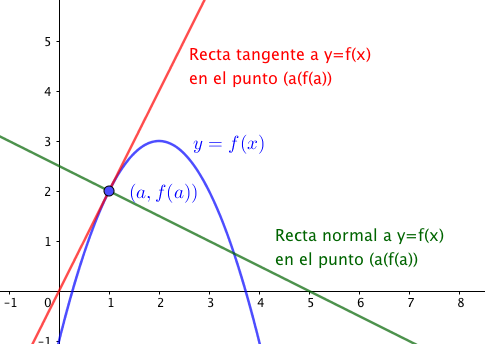
\includegraphics[width=0.4\textwidth]{imagenes/imagenes05/T05IM01.png}
		\caption {Rectas tangente y normal a $f(x)$ en el punto $(a.f(a))$.}
	\end{figure}
	
	 \end{multicols}
	
	Veremos, a continuación cuatro tipos de ejemplos de cálculos de rectas tangentes: el usual, cuando nos dan alguna condición sobre la tangente, cuando la función es implícita, y cuando nos piden que la recta tangente pase por un punto exterior a la curva.
	
	\begin{ejem}
		Calcula la ecuación e la recta tangente a la función $f(x)=\dfrac {3x+2}{2x-1}$ en el punto $x=1$.
		
		En nuestro caso vamos a usar la ecuación \ref{eq:recta-tangente} y para nosotros $a=1 \to $
		$f(1)=5; \quad f'(x)=\dfrac{-7}{(2x-1)^2}; \quad f'(1)=-7$
		
		La ecuación de la recta tangente a $f(x)$ en $x=a=1$ es: $\quad y-5=-7(x-1)$
		
	\end{ejem}
	
	\begin{ejem}
		Encuentra la recta tangente a la función $3x^2+2x+1$ que sea paralela a la recta $r:\; 8x-y+1=0$
		
		La recta $r$, escrita en forma explícita (con la $y$ despejada) es: $y=8x+1$, por lo que su pendiente es $m_r=8$. Recordemos que las rectas paralelas son las que tienen la misma pendiente, así que nuestra recta tangente (RT) buscada ha de ser tal que $m_{RT}=m_r=8$. Pero `la pendiente de la recta tangente a una función en un punto es la derivada en ese punto', (recuerda el `mantra' de la imagen \ref{img:mantra-derivada}). Por todo ello, hemos de buscar un punto $a$ donde trazar la tangente, de modo que $f'(a)=m_{RT}=8$
		
		$y'=f'(x)=6x+2 \to f'(a)=6a+2=8; \; 6a=6;\; a=1$. Hemos de buscar la RT a $f(x)$ en $x=1$: $\quad \Rightarrow y-f(1)=f'(1)\cdot (x-1) \to y-6=8(x-1)$
	\end{ejem}
	
	\begin{ejem}
	Encuentra la ecuación de la recta tangente a la elipse $\dfrac{x^2}{25} + \dfrac {y^2}{16} =1$ en $x_0=4$
	 \begin{multicols}{2}
	 La ecuación \ref{eq:recta-tangente} dice: $y-f(a)=-\dfrac 1 {f'(a)}\cdot(x-a)$. 
	
	Nuestro $a=x_0=4$, tanto para buscar $y(4)=f(4)$ como $y'(4)=f'(4)$, hemos de sustituir en la ecuación de la elipse (podemos encontrar más de una solución) como en la ecuación de la derivada implícita:
	
	$\dfrac 1 {25} 2x + \dfrac 1 {16} 2y\cdot y' =0$ (derivada*).
	
	Si $x=4 \to $ elipse:  $\dfrac {16}{25}+\dfrac {y^2}{16}=1 \to y=\pm 12/5$
	
	Tenemos dos puntos, $(4,\frac {12}{5})$ y $(4,-\frac {12}{5})$ donde sustituir en la ecuación de la derivada implícita (derivada*), para encontrar la $y'(4)=f'(4)$ correspondiente. $(4,\pm\frac {12}{5} \to $ (derivada*) $\to \dfrac 1 {25} 2\cdot 4 + \dfrac 1 {16} 2 \left(\pm 	\dfrac {12}{5}  \right) \cdot y' =0$
	
	Las dos rectas tangentes son:
	
	$x=4;\quad y=\dfrac {12}{5}; \quad y'(4,\dfrac {12}{5})=-\dfrac {16} {5} \Rightarrow  y- \dfrac {12}{5} =-\dfrac {16} {5} \cdot (x-4)$
	
	$x=4;\quad y=-\dfrac {12}{5}; \quad y'(4,-\dfrac {12}{5})=\dfrac {16} {5} \Rightarrow  y+ \dfrac {12}{5} =\; \dfrac {16} {5} \cdot (x-4)$
	
	\begin{figure}[H]
		\centering
		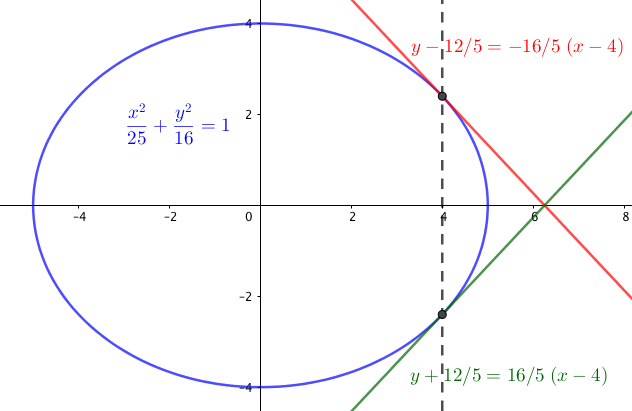
\includegraphics[width=0.5\textwidth]{imagenes/imagenes05/T05IM02.png}
	\end{figure}
	
	
	 \end{multicols}
		
	\end{ejem}
	

	
	\begin{ejem}
		Encuentra la ecuación de la recta tangente a la curva $y=x^2-5x+3$ que pase por el punto (`exterior') $P(2,-7)$.
		
		Comprobamos que, efectivamente, $P(2,-7) \notin y=x^2-5x+3$
	
	Escribamos la ecuación general de la RT a $f(x)$ en un punto arbitrario $x=a$. Luego, determinaremos esa $a$ exigiendo que esa RT pase por el punto  $P(2,-7)$.
	
	$f(a)=a^2-5a+3;\quad f'(x)=2x-5; \; f'(a)=2a-5 \quad \to y-(a^2-5a+3)=(2a-5)\cdot (x-a) \quad \Rightarrow y=(2a-5)x+(3-a^2)\; $: Ecuación de la RT a $f$ en $a$. Hagamos que esta recta pase por $P(2,-7) \to x=2 \leftrightarrow y=-7$:
	
	$-7=(2a-5)2+(3-a^2)\to a^2-4a=0 \to $ Hay dos soluciones $a=0\; \wedge \; a=4$
	
	RT en $x=0 \to f-f(0)=f'(0)(x-0) \to y-3=-5x$
	
	RT en $x=4 \to f-f(4)=f'(4)(x-4) \to y+1=3(x-4)$
	
	Se deja al lector comprobar que ambas rectas pasan por el punto $P(2,-7)$
	
	\end{ejem}



	\begin{defi}{$\divideontimes$  Ángulo que forman dos funciones en el punto de intersección de éstas:}
	
	\begin{figure}[H]
		\centering
		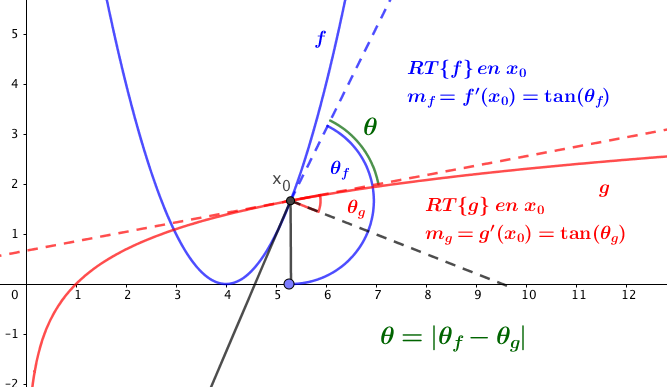
\includegraphics[width=0.7\textwidth]{imagenes/imagenes05/T05IM13.png}
	\end{figure}
	
	Sean $f$ y $g$ dos funciones que se intersectan en $x_0$. Definimos el ángulo que forman entre ellas como aquel que forman sus rectas tangentes en $x_0$:
	
	$\theta =|\theta_{f}-\theta_{g}| \to \tan \theta = \tan |\theta_{f}-\theta_{g}| =\left| \dfrac {\tan \theta_{f}-\tan \theta_{g}}{1+\tan \theta_{f}\; \cdot \; \tan \theta_{g} } \right| = \left| \dfrac {m_r - m_g}{1+m_r \cdot m_g } \right|$
	
	$\qquad \Rightarrow \quad \theta = \arctan \left| \dfrac {f'(x_0)-g'(x_0)}{1+f'(x_0)\cdot g'(x_0)}  \right|$

	\end{defi}

\section[Crecimiento y Extremos Relativos: información obtenida de la primera derivada]{Crecimiento y Extremos Relativos: información obtenida de la primera derivada\sectionmark{Crecimiento y extremos: y'}}
\sectionmark{Crecimiento y extremos: y'}

\label{ExtremosRelativos}

	\begin{defi}
		Se dice que f es `creciente' en $x_0$ si existe un $\delta>0$ de modo que para cualquier $0<h<\delta$, se cumple que $f(x_0-h)\le f(x_0) \le f(x_0+h)$
		
		Si las desigualdades se conservan estrictas, se dice de $f$ es `estrictamente creciente' en $x_0$
		
		La definición es análoga (cambiando el sentido de las desigualdades) para las funciones `decrecientes'.
	\end{defi}
	
	
		
	

	
	\begin{teor}
	$f:]a,b[\to \mathbb R$, derivable en $x_0 \in ]a,b[$	 y tal que $f'(x_0)>0 \Rightarrow f $ es `estrictamente creciente' en $x_0$
	\end{teor}
	
	\begin{proof}
		$f'(x_0)=\underset{h\to 0}{lim}\;{\dfrac {f(x_0+h)-f(x_0)}{h}}>0$. Por el teorema \ref{teor:conserva-signo} de conservación del signo del límite, existirá un entorno de $x_0$ en el que $[f(x_0+h)-f(x_0)]/h>0$, por o que numerador y denominador tendrán el mismo signo.
		\begin{itemize}
			\item Si $h>0$, llamo $h=k: \quad f(x_0+k)-f(x_0)>0 \to f(x_0+k)>f(x_0)$
			\item Si $h<0$, llamo $h=-k: \quad f(x_0-k)-f(x_0)<0 \to f(x_0-k)<f(x_0)$
		\end{itemize}
		
		De ambas desigualdades se deduce que: $f(x_0-k)<f(x_0)<f(x_0+k)$, lo que demuestra que $f$ es `estrictamente creciente' en $x_0$
	\end{proof}
	
	\begin{teor}\label{CS-extremos}
		$f:]a,b[\to \mathbb R$, derivable en $x_0 \in ]a,b[$	 y tal que $f'(x_0)<0 \Rightarrow f $ es `estrictamente decreciente' en $x_0$
	\end{teor}
	
	\begin{proof}
		La demostración es totalmente análoga a la del teorema anterior.
	\end{proof}
	
	\begin{figure}[H]
		\centering
		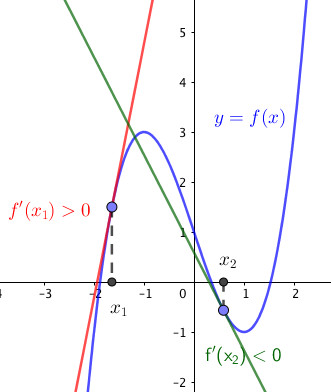
\includegraphics[width=0.5\textwidth]{imagenes/imagenes05/T05IM03.png}
		\caption{$f'(x_1)>0; \; f \mbox{creciente } x_1. \quad  f'(x_2)<0; \; f \mbox{creciente } x_2. $}
	\end{figure}
	
	\underline{Observación}: El que $f'(x_0)>0$ es una condición suficiente, pero no necesaria, para que la función sea estrictamente creciente en $x_0$. Puede que $f'(x)=0 \; \vee \; \nexists f'(x_0) $ y la función sea estrictamente creciente en esos puntos. Ver figura de al lado.
	
	\begin{figure}[H]
		\centering
		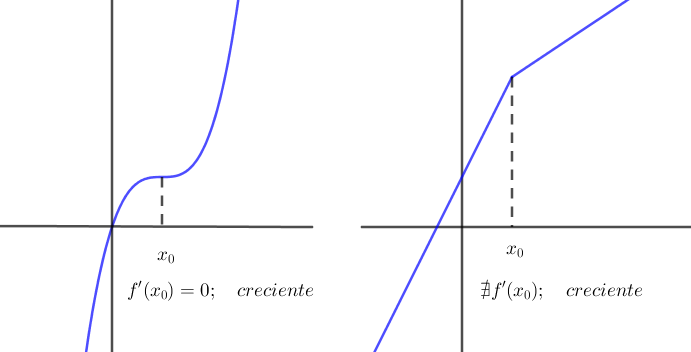
\includegraphics[width=0.7\textwidth]{imagenes/imagenes05/T05IM04.png}
	\end{figure}

	EXTREMOS RELATIVOS.
	
	\begin{defi}
		$f:]a,b[\to \mathbb R; \; x_0\in ]a,b[$. Se dice que $f$ tiene un `máximo relativo o local' en $x_0$ si existe un $\delta>0 \; / \; f(x)\le f(x_0), \; \forall x \in E_{\delta}(x_0)=]x_0-\delta, x_0+\delta[$
	\end{defi}
	
	\begin{defi}
		Análogamente, sea $f:]a,b[\to \mathbb R; \; x_0\in ]a,b[$. Se dice que $f$ tiene un `mínimo relativo o local' en $x_0$ si existe un $\delta>0 \; / \; f(x)\ge f(x_0), \; \forall x \in E_{\delta}(x_0)=]x_0-\delta, x_0+\delta[$
	\end{defi}

	
	\begin{defi}
	$f:]a,b[\to \mathbb R; \; x_0\in ]a,b[$. Se dice que $f$ tiene un `extremo relativo' en $x_0$ si $f$ presenta en $x_o$ un `máximio un `mínimo'.	
	\end{defi}
	
	En un máximo, $x_M$, la función pasa de ser creciente a su izquierda a decreciente a su derecha, lo contrario ocurre con un mínimo, $x_m$, que la función pasa de decreciente a creciente al atravesar a $x_m$ de izquierda a derecha.
	
	\begin{teor}
		$f:]a,b[\to \mathbb R; \; x_0\in ]a,b[;\ f\; $ derivable en $x_0$ y $x_0\; $ extremo de $\; f \Rightarrow f'(x_0)=0$.
	\end{teor}
	\begin{proof}
		Si $f$ es derivable en $x_0$, siendo $x_0$ extremo de $f$, tenemos:
		\begin{itemize}
			\item $f$ no es creciente en $x_0 \to f'(x_0)\ngtr 0$
			\item $f$ no es decreciente en $x_0 \to f'(x_0)\nless  0$
		\end{itemize}
		Necesariamente, si $\exists f'(x_0)$ y no puede ser ni mayor ni menor que cero: $f'(x_0)=0$
	\end{proof}

	%\begin{multicols}{2}

	La condición necesaria para que una función tenga un máximo o mínimo (extremo) relativos en $x_0$ es que su primera derivada en dicho punto se anule, $f'(x_0)=0$, pero esta condición no es suficiente. Valgan, como contraejemplos, las funciones $x^3$ con derivada nula en $0$, pero creciente en $0$, no es extremo; y la función $|x|$ que sí tiene un mínimo relativo en $0$ pero $f'(0)\neq 0; \; \nexists f'(0)$.
	
	\begin{figure}[H]
		\centering
		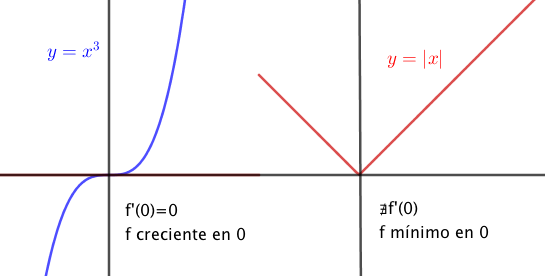
\includegraphics[width=0.6\textwidth]{imagenes/imagenes05/T05IM05.png}
	\end{figure}
	
	%\end{multicols}
	
	\begin{defi} PUNTOS CRÍTICOS:  Llamamos puntos críticos de la primera derivada, $PC(y')$ a aquellos puntos en que o bien $y'=f'(x)=0$, o bien $\nexists y; \; \nexists f'(x)$.
	\end{defi}
	
	\begin{multicols}{2}
	 
	\begin{figure}[H]
		\centering
		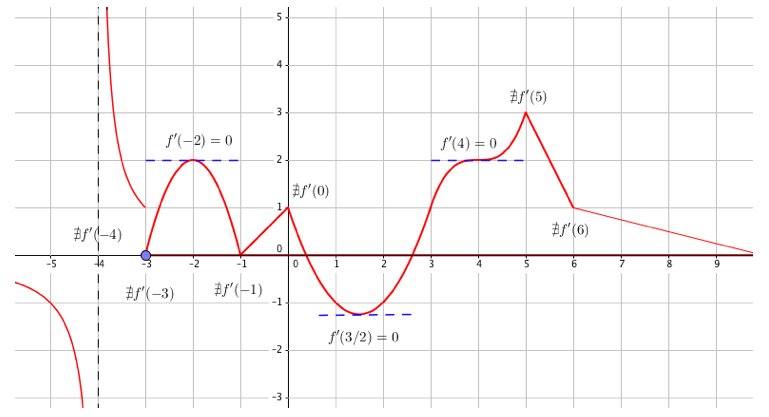
\includegraphics[width=0.5\textwidth]{imagenes/imagenes05/T05IM06.png}
	\end{figure}
	
	La figura muestra que los posibles extremos relativos de la función se producen en los puntos críticos de su primera derivada. Ello nos servirá como procedimiento para encontrar los extremos relativos de una función. Los $PC(f')$ serán los `candidatos' a máximos o mínimos.
	
	\end{multicols}
	
	ALGORITMO PARA ENCONTRAR LOS EXTREMOS DE UNA FUNCIÓN:	
	
	\begin{enumerate}
		\item Calculamos $y'=f'(x)$
		\item Buscamos los $PC(y')=\begin{cases}
							y'=0 \to x_1, x_2, \cdots \\
							\nexists y' \to x_3, x_4, \cdots	
							\end{cases}$
		\item Se tabulan en la recta $\mathbb R$ los puntos críticos obtenidos y se estudia, en los intervalos que aparecen, el signo que toma $y'$. Donde $y'>0 \to y \nearrow $ (creciente) ;  Donde $\;  y'<0 \to y \searrow $ (decreciente). Si en un determinado punto la función cambia su crecimiento, tendremos un extremo.
	\end{enumerate}
	
	La siguiente imagen intenta explicar como determinar los extremos de la imagen anterior.
	
	
	\begin{figure}[H]
		\centering
		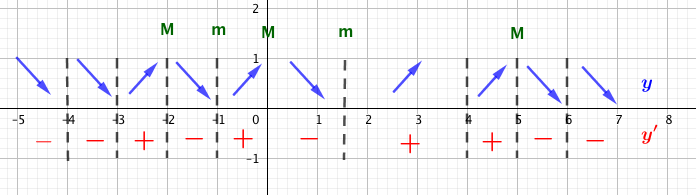
\includegraphics[width=0.9\textwidth]{imagenes/imagenes05/T05IM07.png}
	\end{figure}
	
	\begin{ejem} Calcula los intervalos de crecimiento y de decrecimientos, así como los extremos relativos de la función:  $f(x)=x^3-6x^2+9x$
	
	\noindent \small{$y'=f'(x)=3x^2-12 x+9 \to PC(y') =\begin{cases}
	y'=0 \to 3x^2-12x+9=0 \to x=1 \; \wedge \; x=3 \\
	\nexists y' \ \nexists x \mbox{ siempre existe y'}
	\end{cases}$}
	
	\normalsize{Los} $PC(y')$ son el $1$ y el $3$, lo representamos en una tabla y estudiamos el signo de la primera derivada (crecimiento de la función) en los intervalos que aparecen:
	
	\begin{table}[H]
	\centering
	\begin{tabular}{|c|c|c|c|c|c|}
	\hline
	Crecto. &$]-\infty,1[$  & $1$ & $]1,3[$ & $3$ & $]3,+\infty[$ \\ \hline
 	$f':\; $ &  $+$ & $0$ & $-$ & $0$ & $+$ \\ \hline
 	$f;\;$ & $\nearrow$  & $M(1,4)$ & $\searrow$ & $m(3,0)$ & $\nearrow$ \\ \hline
	\end{tabular}
	\end{table}
	
	Muchos autores dan la información, para mi redundante, siguiente:
	
	\hspace{10mm} $f \mbox{ es creciente en} ]-\infty,3[\cup ]3,+\infty[$
	
	\hspace{10mm} $f \mbox{ es decreciente en} ]-1,-3[$
	
	\hspace{10mm}  $F \mbox{ tiene un } M(1,4) \mbox{ y un } m(3,0)$
	
	Considero toda esta información redundante porque se observa directamente de la tabla anterior (o gráfico, como veremos en ejemplos posteriores) .
	
		
	\end{ejem}
	
	\begin{ejem} Calcula los intervalos de crecimiento y de decrecimientos, así como los extremos relativos de la función:  $f(x)=\dfrac{x^3}{x^2-1}$
	
	$y'=\dfrac {x^4-3x^2}{(x^2-1)^2}$
	$\to PC(y')=\begin{cases}
	y'=0 \to x^2(x^2-3=0 \to x=0;\; x=\pm \sqrt{3} \\
	\nexists y' \to (x^2-1)^2=0 \to x^2-1=0\to x=\pm 1
	\end{cases}$
	
	\begin{table}[H]
	\centering	
	\begin{tabular}{|c|c|c|c|c|c|}
	\hline
 	Crecto.& $]-\infty,-\sqrt{3}[$ & $-\sqrt{3}$ & $]-\sqrt{3},-1[$ & $-1$ & $]-1,0[$ \\ \hline
 	$f':\;$& $+$ & $0$ & $-$ & $\nexists$ & $-$ \\ \hline
 	$f:\;$& $\nearrow$ & $M(-\sqrt{3},-3\sqrt{3}/2)$ & $\searrow$ & $AV$ & $\searrow$ \\ \hline
	\end{tabular}
	\end{table}
	
	\begin{table}[H]
	\centering	
	\begin{tabular}{|c|c|c|c|c|c|c|}
	\hline
 	(sigue)& $0$ & $]0,1[$ & $1$ & $]1,\sqrt{3}[$ & $\sqrt{3}$ & $]\sqrt{3},+\infty[$ \\ \hline
 	$f':\;$& $0$ & $-$ & $\nexists$ & $\-$ & $0$ & $+$\\ \hline
 	$f:\;$& $I(0,0)(*)$ & $-$ & $AV$ & $-$ & $m(\sqrt{3},3\sqrt{3}/2)$ & $\nearrow$\\ \hline
	\end{tabular}
	\end{table}
	
	En el punto $(0,0)$ la función, aunque $f'(0)=0$, no tiene ni M ni m, hay un `punto de inflexión', algo que estudiaremos con la segunda derivada.
	
	\end{ejem}

	\begin{ejem} Calcula los intervalos de crecimiento y de decrecimiento, así como los extremos relativos de la función:
	\label{ejem:extremos-trozos}
	
	$f(x)=\begin{cases}
	  2 & \mbox{ si } x\le -4  \\
	   x + 2& \mbox{ si }  -4<x<2 \\
	 4-x^2 & \mbox{ si } -2 \le x \le <2  \\
	  x-2 & \mbox{ si } 2< x <6  \\
	  10-x& \mbox{ si } x>6   
	\end{cases} \to 
	f'(x)=
	\begin{cases}
	  0 & \mbox{ si } x< -4  \\
	  1 & \mbox{ si }  -4<x < -2 \\
	 -2x & \mbox{ si } -2<x<2  \\
	  1 & \mbox{ si } 2 < x < 6  \\
	  -1 & \mbox{ si } x>6   
	\end{cases}
	$
	
	\noindent Estudiaremos primero la continuidad para decidir si $\mbox{ ?` } \exists f'(-4), f'(-2), f'(2), f'(6) \mbox { ? }$
	
	La función es continua en todo $\mathbb R$ por ser todo trozos polinómicos excepto, tal vez, en los nexos o nodos de función donde hay que estudiar  la continuidad. Un estudio rápido (rigurosamente hay que hacer el método de los tres pasos para cada nexo) releva que:
	
		
	\begin{itemize}

	\item $f_-(-4)=2 \neq -2 =f_+(-4) \to f $ discontinua salto en $x=-4 \to \nexists  f'(-4)$. 
	
	\item $f_-(-2)=0=f'_+(-4) \to f $ continua en $x=-2:\quad f'_-(-2)=1	\neq f'_+(-2)=4 \to \nexists f'(-2)$ En $x=-2$ hay un punto anguloso $PA$.
	
	\item $f_-(2)=0=f_+(2) \to f $ continua en $x=2:\quad f'_-(2)=-4 	\neq f'_+(2)=1 \to \nexists f'(2)$ En $x=2$ hay un punto anguloso $PA$.
	
	\item $f_-(-6)=4=f_+(6) \to f $ continua en $x=6:\quad f'-(6)=1 \neq -1 =f'_+(6)$. En $x=6$ hay un $PA$. 
	
	$PC(y')$: Veamos cuando $y'=0$ y cuando $\; \nexists y'$:
	
	$\nexists \; y'$ cuando $x=-4$, pero no nos importa ya que no es continua en él; también  $\nexists \; y'$  en $x \in \{-2, 2 , 6\}$
	
	$y'=0 \to \begin{cases}
	x<-4: & y':\; 0 \;  \forall x<-4 \to \tiny{\mbox{f cte., ni M ni m}} \normalsize{.} \\
	-4<x<-2  & y':\;  1 \neq 0 \\
	-2<x<2 & y':\;  -2x=0 \to x=0 \\
	2<x<6 & y':\;  1 \neq 0 \\
	x>6 & y':\;  -1 \neq 0
 	\end{cases} $
 	
 	$ f'(x)=0 \to x=0$

	Hemos de estudiar el signo de $f'(x)$ en los segmentos en que $\{-2, 0, 2 , 6\}$ dividen a $\mathbb R$. En este caso usaremos un gráfico en vez de una tabla para que el lector pueda comparar su sencillez.
	
	
	\end{itemize}
	
	
	\begin{figure}[H]
		\centering
		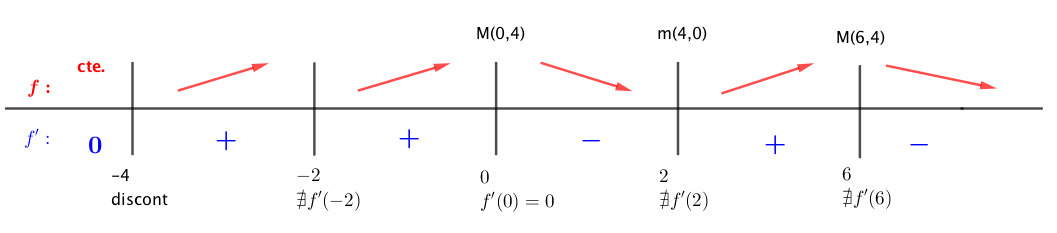
\includegraphics[width=1\textwidth]{imagenes/imagenes05/T05IM09.png}
	\end{figure}
			
	\end{ejem}


	\subsection{Extremos Absolutos}
	
	Los \emph{`extremos absolutos'} de $y=f(x)$ en un intervalo cerrado $[a,b]$, como es obvio (véase la imagen adjunta) se alcanzarán en los extremos relativos de $f$ en $]a,b[$, o en los límites del intervalo $x=a$ , $x=b$. Por ello, para estudiar \emph{`extremos absolutos'} de $y=f(x)$ en un intervalo cerrado $[a,b]$ procederemos buscando los puntos críticos de la primera derivada en el intervalo abierto $PC(y')\in\;  ]a,b[$ y tabulado la función en esos valores encontrados y, también, en $x=a$ y en $x=b$. Donde $y=f(x)$ tomo el valor más grande, tendremos el `máximo absoluto' y donde alcance el más pequeño, el `mínimo absoluto'. Todo ello puede ocurrir en más de un punto.
	
	
	\begin{figure}[H]
		\centering
		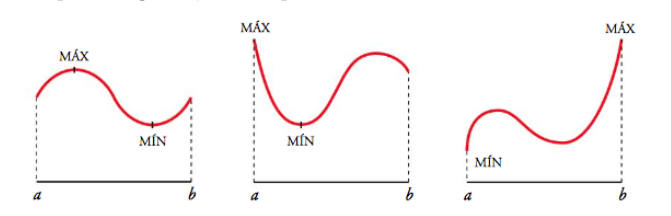
\includegraphics[width=1\textwidth]{imagenes/imagenes05/T05IM08.png}
		\caption{Extremos absolutos de $f(x)$ en $[a,b]$.}
	\end{figure}
	
	
	\begin{ejem} Calcula los extremos Absolutos de la función:  $f(x)=x^3-6x^2+9x$ en los intervalos:
	
	$\quad a)\; [0,4] \qquad b)\; [0,5]$
	
	Procedemos, en principio igual que para buscar extremos relativos, buscamos $PC(y')$:
	
	$y'=f'(x)=3x^2-12 x+9 \to $
	
	$PC(y') =\begin{cases}
	y'=0 \to 3x^2-12x+9=0 \to x=1 \; \wedge \; x=3 \\
	\nexists y' \ \to  \nexists x ; \mbox{ siempre existe y'}
	\end{cases}$
	
	Ahora, para cada intervalo pedido, hemos de tabular la función $y=f(x)$ en los extremos relativos de $y'$ interiores al intervalo y en los límites de éstos.
	
	\begin{table}[H]
	\centering
	\begin{tabular}{|c|c|c|c|c|c|c|c|c|c|c|}
	\cline{1-5} \cline{7-11}
	 $a) \; \;  x$& 0& 1 & 3 & 4 & $\qquad$ & $b)\; \;  x$ & 0 & 1 & 3  & 5 \\ \cline{1-5} \cline{7-11} 
 	$y=f(x)$& 0 & 4 & 0 & 4 & $\qquad$ &$ y=f(x)$  & 0 & 4 & 0 & 20 \\ \cline{1-5} \cline{7-11} 
	\end{tabular}
	\end{table}
	
	En el apartado $a)$, intervalo $[0,4]$, la función alcanza el máximo absoluto, de valor $4$, en dos puntos, $x=1 \; \wedge \; x=4$ y alcanza el valor mínimo absoluto, de valor $0$, también en dos puntos $x=0\; \wedge \; x=3$.
	
	En el apartado $b)$, intervalo $[0,5]$, la función alcanza el máximo absoluto, de valor $20$, en el punto, $x=5$ y alcanza el valor mínimo absoluto, de valor $0$, también en dos puntos $x=0\; \wedge \; x=3$.
	
	\end{ejem}
	
	\begin{ejem}
		Calcula los extremos Absolutos de la función:  $f(x)$ en los intervalos $a)\; [-2,3]$ y $b)\; [-2,7]$
		
		\noindent $f(x)=\begin{cases}
		4-x^2 & \mbox { si }	 -2 \le x \le 2 \\
		x-2 & \mbox{ si } x>2
	\end{cases} \quad \to$
	$f'(x)=\begin{cases}
	-2x & \mbox { si }	 -2<x<2 \\
	1 & \mbox { si }	 x>2
	\end{cases} \quad \mbox{ ?`}\exists f'(2)?$
	
	Por abreviar, como en el ejemplo \ref{ejem:extremos-trozos}, hemos derivado la función en los intervalos abiertos. Estudiamos a continuación la continuidad y la derivavibilidad en los nexos.
	
	La función ex continua en $[-2,+\infty]$ que es su dominio de definición y también en el nexo: $f_-(2)=0=f_+(2)$, continua en $x=2$.
	
	$f'_-(2)=-4 \neq f'_+(2)=1 \to x=2 ; \; \nexists f'(2)$
	
	$f'(x)=0$ solo en $-1<x<2: \to  -2x=0 \to x=0$
	
	Los $PC(y')$ son $\{-2,0\}$. Estudiemos los extremos absolutos tabulando la función en los $PC(y')$ en el interior de los intervalos considerados y en los límites de los mismos:
	
	\begin{table}[H]
	\centering
	\begin{tabular}{|c|c|c|c|c|c|c|c|c|c|c|}
	\cline{1-5} \cline{7-11}
	 $a);\ \;  x$& -2& 0 & 2 & 3 & $\qquad$ & $b)\; \;  x$ & -2 & 0 & 2  & 7 \\ \cline{1-5} \cline{7-11} 
 	$y=f(x)$& 0 & 4 & 0 & 1 & $\qquad$ &$ y=f(x)$  & 0 & 4 & 0 & 5 \\ \cline{1-5} \cline{7-11} 
	\end{tabular}
	\end{table}
	
	
	Por lo que $f(x)$ en $[-2,3]$ alcanza el máximo absoluto en el punto $MA(0,4)$ y en mínimo absoluto en los puntos $mA(\pm 2,0)$.
	
	$f(x)$ alcanza en $[-2,7]$ el máximo absoluto en el punto $MA(7,5)$ y en mínimo absoluto en los puntos $mA(\pm 2,0)$.

	
	\end{ejem}
	
	\begin{teor} Criterio de la derivada segunda para la determinación de máximos y mínimos.
	\label{teor-crit-deriv2}
		
		Sea $f:]a,b[ \to \mathbb R: \; / \; f'(x_0)=0, \; \mbox{ con } x_0\in \; ]a,b[ \Rightarrow$
		
		\begin{itemize}
			 \item $\qquad \mbox{ si } f''(x_0)<0 \to f $ tiene un `máximo' en $x_0$.
			\item $\qquad \mbox{ si } f''(x_0)>0 \to f $ tiene un `mínimo' en $x_0$.
		\end{itemize}
		
	\end{teor}
	
	\begin{proof}
		Si $f''(x_0)<0 \to y'=f'(x)$ será decreciente en $x_0$, como $f'(x_0)=0$, deberá ocurrir que $\exists \delta>0: \; f'(x_0-\delta)>f'(x_0)>f'(x_0+\delta)$, por lo que $f$ es creciente en puntos $x_0-\delta$ y en decreciente en puntos $x_0+\delta$: como en $x_0$ la función para de ser creciente a su izquierda a decreciente a su derecha, en $x_0$ hay un `máximo'.
		
		La demostración es análoga para el caso de que $f''(x_0)>0$, en $x_0$ habrá un `mínimo'.
		
		\begin{figure}[H]
		\centering
		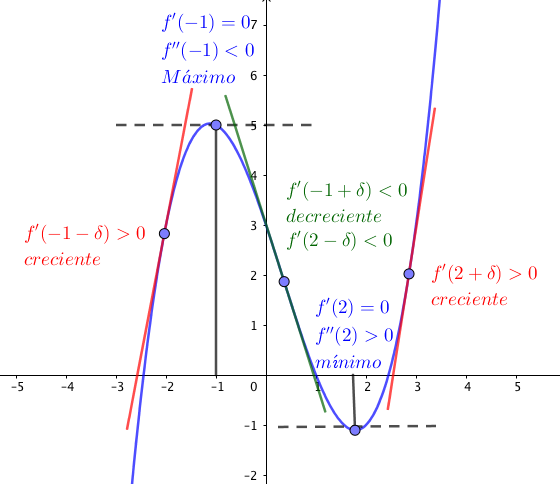
\includegraphics[width=.5\textwidth]{imagenes/imagenes05/T05IM10.png}
		\caption{Criterio de la segunda derivada para M y m.}
	\end{figure}
		 
	\end{proof}

	
	
	\subsection{Optimización de funciones}
	
	En muchas esferas de la actividad humana surgen, frecuentemente, \emph{problemas de optimización}, es decir, problemas que obligan a encontrar los valores necesarios de algunas variables para que una determinada magnitud $F$ alcance el valor óptimo (M o m).
	
	Piénsese, p.e., en una fábrica donde se quieren enlatar conservas en botes cilíndricos de $1 \; l$ de capacidad. Lógicamente les aparecerá el problema de averiguar las dimensiones del bote que resulte más barato de fabricar. La lata óptima será la que, conteniendo el $1 \; l$ de capacidad, tenga superficie total mínima, por lo que se necesitará menos material para su fabricación.
	
	En este caso se desea averiguar los valores de las variables $r$ (radio) y $h$ (altura) del bote, para que la magnitud $S$ (superficie total del bote) sea mínima. Evidentemente $r$ y $h$ no pueden ser cualesquiera, pues han de cumplir con la condición de que el volumen de la lata sea $1 \; l$.
	
	En muchos casos, estos problemas de optimización se resuelven por el siguiente método:
	
	\begin{itemize}
		\item Si $F$ es la magnitud a optimizar, se expresa $F$ en función de las variables que la definen $F=F(x,y,z,\cdots)$.
		\item Las variables $x,y,x,\cdots$ se expresan en función de una sola de ellas, p.e. $x$. Normalmente, los datos del problema permiten hacerlo.
		\item Con esto, la magnitud $F=F(x)$ quedará como función de una sola variable (que es la parte del análisis a que está dedicado este libro, existe también el análisis matemático en varias variables). Entones, para encontrar los valores óptimos o extremos, procederemos como ya sabemos de apartados anteriores: buscando los $PC(F')$ y, según estemos en un intervalo cerrado o no, procederemos como hemos aprendido.
		\item El problema acaba al reinterpretar el resultado final obtenido.
	\end{itemize}
	
	\begin{ejem} En una fábrica donde se quieren enlatar conservas en botes cilíndricos de $1 \; l$ de capacidad, encontrar las dimensiones del bote que resulte más económico en cuanto a materia prima para su fabricación (el que disponga de superficie total mínima).
	
	\begin{multicols}{2}
	
	\begin{figure}[H]
		\centering
		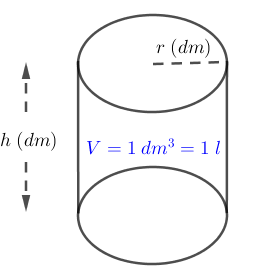
\includegraphics[width=.2\textwidth]{imagenes/imagenes05/T05IM11.png}
	\end{figure}
	
	$V=\pi\; r^2\; h \; (dm^3) = \pi\; r^2\; h \; (l) = 1 \; (l)$
	
	$ \to h=\dfrac {1}{\pi \; r^2 \quad}$ (*)

	$h \; (dm); \; \; r\; (dm)$
	
	
	\end{multicols}

	$S(r)=2S_B+S_L=2\pi r^2+2\pi r h=(*)=2\pi r^2 + 2 \pi r \dfrac {1}{\pi r^2}=2\pi r^2 + \dfrac 2 r$
	
	$S'(r)=4\pi r - \dfrac 2 {r^2} \to PC(y')= \begin{cases}
 	y'=0 \to r^3 = \dfrac {1}{2 \pi} \to r=\sqrt[3]{\dfrac {1}{2 \pi}} \approx 0.54\; dm \\
 	\nexists y' \to r=0
 	\end{cases}$	
 	
 	Puesto que las condiciones del problema nos imponen $r \in \mathbb R_*^+=]0,+\infty[$, el único punto crítico es $r=0.54$. Representando en $\mathbb R$.
 	
 	\begin{multicols}{2}
 	
 	La mínima superficie se alcanza para $r=0.54\; dm$, por (*) $\; h=1.08\; dm$, y el área mínima es de $S(0.54)=5.5\; dm^2$. Obviamente para $V=1\; l$
 	
 	\begin{figure}[H]
	\centering
	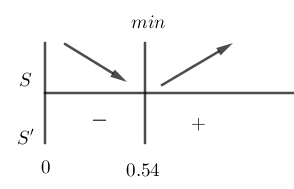
\includegraphics[width=.3\textwidth]{imagenes/imagenes05/T05IM12.png}
	\end{figure}
	
 	\end{multicols}
 	
 	Nótese la curiosidad de que en este bote de área mínima prácticamente coinciden la altura con el diámetro.

	\end{ejem}

	
\section[Curvatura (concavidad y convexidad) e Inflexiones: información obtenida de la segunda derivada]{Curvatura (concavidad y convexidad) e Inflexiones: información obtenida de la segunda derivada\sectionmark{Curvatura e Inflexiones: y''}}
\sectionmark{Curvatura e Inflexiones: y''}


	$f$ drvble. en $]a,b[$ y $x_0\in ]a,b[$
	
	\begin{defi} $f$ es `cóncava' en $x_0$ $\; (\cup)\; $ si en un entorno de $x_0$ la tangente se encuentra por debajo de la función ($f`(x)$ es creciente en $x_0$).
		
	\end{defi}
	
	\begin{defi} $f$ es `convexa' en $x_0$ $\; (\cap)\; $ si en un entorno de $x_0$ la tangente se encuentra por encima de la función ($f`(x)$ es decreciente en $x_0$).
		
	\end{defi}

	
	\begin{figure}[H]
	\centering
	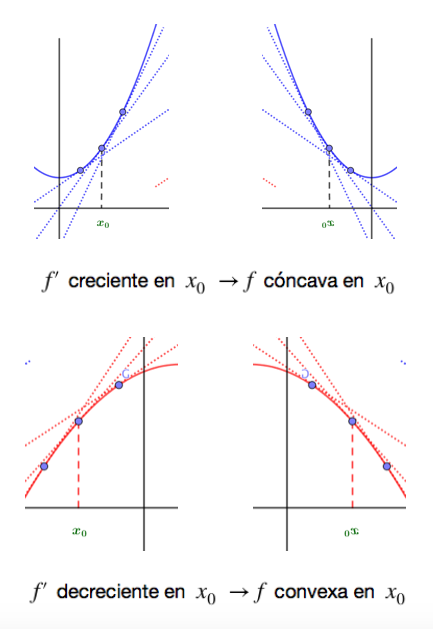
\includegraphics[width=.5\textwidth]{imagenes/imagenes05/T05IM14.png}
	\end{figure}
	
	

	\begin{teor} Curvatura (concavidad y convexidad) y segunda derivada.
	\begin{multicols}{2}
		\begin{itemize} 
			\item si $f''(x_0)>0 \to f \mbox { cóncava en }  x_0 \ \cup; $
			\item si $f''(x_0)<0 \to f \mbox { convexva en }  x_0 \; \cap$
		\end{itemize}
		\begin{figure}[H]
		\centering
		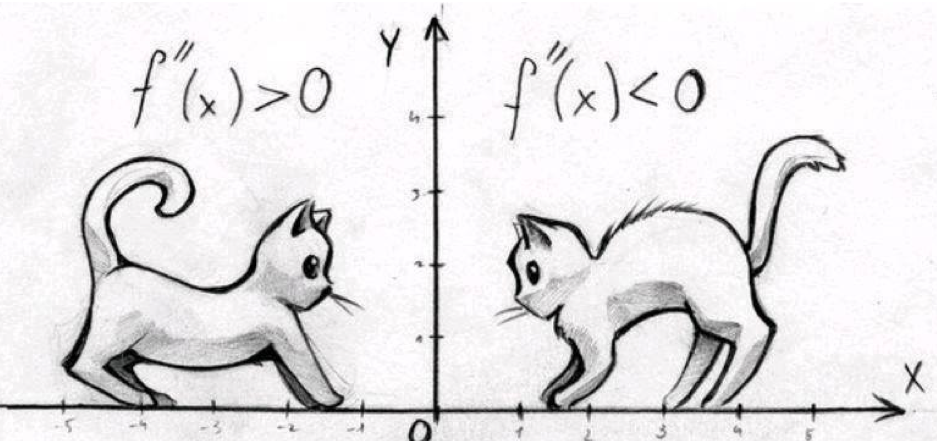
\includegraphics[width=0.35\textwidth]{imagenes/imagenes05/xiste05.png}
		\end{figure}
	\end{multicols}
		
	\end{teor}
	Muchos autores prefieren hablar de curvatura o concavidad hacia arriba $(\cup)$ y de curvatura o concavidad hacia abajo $(\cap)$ en lugar de concavidad y convexidad directamente. 
	
	\emph{Es fácil recordar que lo positivo en esta vida ($f''(x_0)>0)$ es la felicidad $(\cup,\; $ sonrisa).}
	
	\begin{proof}
		Si $f''(x_0)>0 \to y'=f'(x)$ es, como función, creciente en $x_0$ y las tangentes quedan por debajo de la curva.
	\end{proof}

	
		
	

	
	\begin{defi} Punto de Inflexión.
	
	$x_0$ es un $PI$ de $f$ si la recta tangente a $f$ en $X_0$ atraviesa a la gráfica de $f$, para cualquier entorno de $x_0$. En estos puntos la función no es ni cóncava ni convexa sino que pasa de ser una cosa a la otra al pasar de izqda. a la dcha. de $x_0$
	\end{defi}
	
	
	
	\begin{teor} Si $x_0$ es $PI$ de $f \to f''(x_0)=0$.
	
	Esta condición es necesaria pero no suficiente. También se puede presentar una inflexión en puntos de no derivabilidad de la función (PA). Lo veremos en el siguiente ejemplo.
		
	\end{teor}
	
	
	
	\begin{proof}
	Usaremos una figura que lo aclare.
	
	\begin{multicols}{2}
	
$\quad$
	
		Obvio, pues a la derecha e izquierda de $x_0$ la función cambia su concavidad, la segunda derivada pasará de ser $+$ a $-$ al pasar de izqda. a dcha. de $x_0$ o al revés.
	
	\begin{figure}[H]
	\centering
	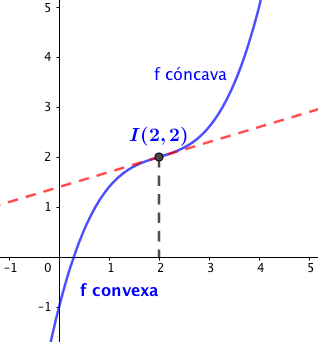
\includegraphics[width=.25\textwidth]{imagenes/imagenes05/T05IM15.png}
	\end{figure}
	\end{multicols}
	\end{proof}
	
	ALGORITMO PARA ENCONTRAR LAS INFLEXIONES DE UNA FUNCIÓN:	
	
	\begin{enumerate}
		\item Calculamos $y''=f''(x)$
		\item Buscamos los $PC(y'')=\begin{cases}
							y''=0 \to x_1, x_2, \cdots \\
							\nexists y'' \to x_3, x_4, \cdots	
							\end{cases}$
		\item Se tabulan en la recta $\mathbb R$ los puntos críticos obtenidos y se estudia, en los intervalos que aparecen, el signo que toma $y''$. Donde $y''>0 \to y \; \cup $ (cóncava) ;  Donde $\;  y''<0 \to y \; \cap  $ (convexa). Si en un determinado punto la función cambia su curvatura (concavidad o convexidad), tendremos un punto de inflexión.
	\end{enumerate}

	\begin{ejem} Estudia la curvatura e inflexiones de 
	
	$f(x)=\begin{cases}
		|x^2-4| & \mbox{ si } x<3 \\
		x^2-10x+25 & \mbox{ si } x\ge 3
		\end{cases}$
		
	$y=f(x)=\begin{cases}
	x^2-4 & \mbox{ si } x<-2 \\
	4-x^2 & \mbox{ si } -2\le x \le 2 \\
	x^2-4 & \mbox{ si } 2<x<3 \\
	x^2-10x+26 & \mbox{ si } x\ge 3
	\end{cases} $ 
	
	Se deja a lector comprobar que $f(x)$ es ctna. en todo $\mathbb R$	
	
	$y=f'(x)=\begin{cases}
	2x & \mbox{ si } x<-2 \\
	-2x & \mbox{ si } -2< x < 2 \\
	2x & \mbox{ si } 2<x<3 \\
	2x-10 & \mbox{ si } x> 3
	\end{cases} \qquad \nexists f'(-2); \; \nexists f'(2); \nexists f'(3);$  
	
	Son 3 puntos angulosos, donde $\nexists f'(x)$; además, $f'(x)=0 \leftrightarrow x=0 \; \wedge \; x=5$. Esto sería necesario si deseáramos encontrar los extremos relativos de $f(x)$, así como sus intervalos de crecimiento y decrecimiento.
	
	$y=f''(x)=\begin{cases}
	2 & \mbox{ si } x<-2 \\
	-2 & \mbox{ si } -2< x < 2 \\
	2 & \mbox{ si } 2<x<3 \\
	2 & \mbox{ si } x> 3
	\end{cases} \qquad \nexists f''(-2); \; \nexists f''(2); \nexists f''(3)$  
	
	Tenemos como $PC(y'')=\begin{cases}
	y''=0 \to \nexists x \mbox{ la y'' no se anula}  \\
	\nexists f''(x) \to x \in \{-2,2,3\} \mbox{ (ya no existía y') }
	\end{cases}
	$
		
	\begin{figure}[H]
	\centering
	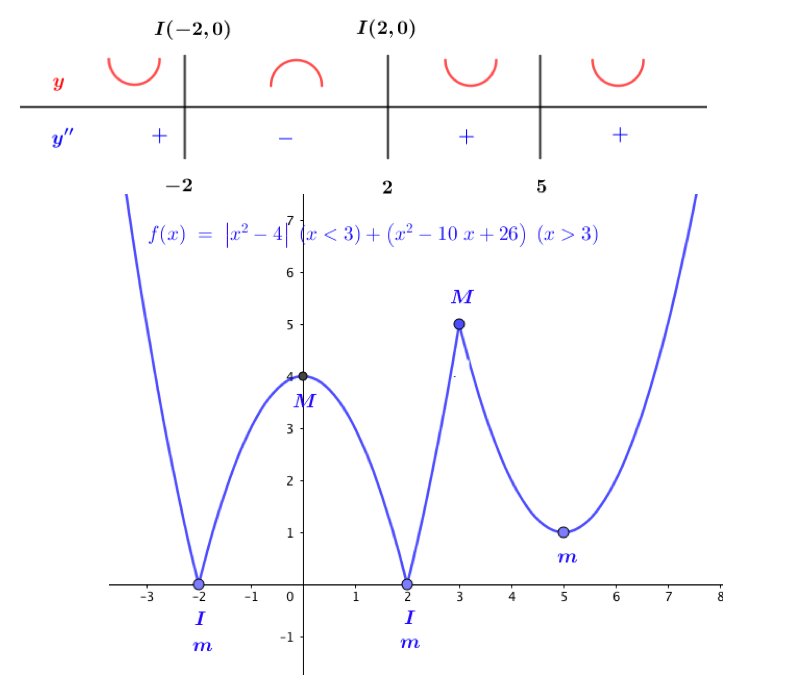
\includegraphics[width=.7\textwidth]{imagenes/imagenes05/T05IM16.png}
	\end{figure}
			
	\end{ejem}
	
	\begin{ejem}
	Calcula la Curvatura e Inflexiones	de $f(x)=x^5+2x$
	
	$y=x^5+2x \to y'=5x^4+2 \to y''=20x^3 \to PC(y'')=\begin{cases}
	y''=0 \leftrightarrow x=0 \\
	\nexists y'' : \; \nexists x
	\end{cases}$
	
	Evidentemente, para $x<0:\; y''<0$ y para $x>0: \; y''>0$, la función pasa de tener concavidad hacia abajo (convexa) a la izquierda del cero a concavidad hacia arriba (cóncava) a la derecha del cero, en $x=0$ hay pues un `punto de inflexión:' $I(0,f(0))=I(0,0)$.
	\end{ejem}


\section{Ejercicios de aplicaciones de las derivadas}
\subsection{Ejercicios resueltos de aplicaciones de las derivadas}

\underline{Rectas tangente y Normal.}

	\begin{ejre}
			Considera las funciones $f(x)=x^2-2x+3$ y $g(x)=ax^2+b$. Calcula:
			
			$\qquad a) \; $ $a$y $b$ para que las gráficas de $f$ y $g$ sean tangentes en el punto de abcisa $x=2$
			
			$\qquad b) \;$ Para los valores encontrados, busca la ecuación de la recta tangente común a ambas funciones. 
			
	\end{ejre}
		
	\begin{proofw}\renewcommand{\qedsymbol}{$\diamond$}
	
	Obviamente, las funciones son ctnas. y dervbles. en todo $\mathbb R$ por ser funciones polinómicas.
	
	Calculemos las derivadas en $x=2:\quad f'(x)=2x-2;\; f'(2)=2; \quad g'(x)=2ax; \; g'(2)=4a\; $ Las gráficas de $f$ y $g$ serán tangentes en $x=2$ si lo son sus rectas tangentes (forman ángulo cero, tienen la misma pendiente), por ello $f'(2)=g'(2) \to 2=4a \to a=1/2$
	Busquemos las rectas tangentes y veremos que son iguales: $f(2)=3$; $g(2)=2+b\; (a=1/2)$. Como las dos rectas han de pasar por el mismo punto $3=2+b \to b=1$
	
	$RT$ a $f$ en $x=2\qquad \to \qquad y-3=2(x-2) \to y=2x+1$
	
	$RT$ a $g$ en $x=2\qquad \to \qquad y-3=2(x-2) \to y=2x+1 \qquad (a=1/2 \; \wedge b=1)$
	
	\end{proofw}
	
	\begin{ejre}
	Dada la función $f(x)=\ln \left( \dfrac {x^2}{x-1} \right)$, definida para $x>1$, encuentra un punto $(a,f(a))$ tal que la recta tangente a la gráfica de $f(x)$ en ese punto sea paralela al eje $OX$.	
	\end{ejre}
	
	\begin{proofw}\renewcommand{\qedsymbol}{$\diamond$}

		Dos rectas son paralelas si tienen la misma pendiente. La ecuación del eje $OX$ es $y=0$, por lo que $m_{OX}=0$. Buscamos pues, un punto $a$ en que $m_{RT(a)}=f'(a)=0$.
		
		$y'=f'(x)= \dfrac {\cancel{x-1}}{x^2} \cdot \dfrac {2x(x-1)-x^2\cdot 1}{(x-1)^{\cancel{2}}}=\dfrac {\cancel{x}(x-2)}{x^{\cancel{2}}(x-1)}=\dfrac {x-2}{x(x-1)}$
		
		$f'(a)=0 \to \dfrac {a-2}{a(a-1)}=0 \to a-2=0 \to a=2; \quad f(2)=\ln 4$
		
		El punto pedido es $(2,\ln4)$ y la $RT$ es $y-	\ln4=0(x-2) \to y=\ln4$, función constante, recta horizontal, pendiente cero, paralela al eje $OX$.
		
	\end{proofw}

	\begin{ejre}
		Se considera la función $f(x)=x^2+m$, donde $m>0$ es una constante.
		
		$\qquad a) \; $Para cada valor de $m$ encuentra el valor de $a>0$ tal que la RT en $(a,f(a))$ pase por el origen de coordenadas.
		
		$\qquad b) \; $ Hallar el valor de $m$ para que la recta $y=x$ sea tangente a la gráfica f(x).
	\end{ejre}
	
	\begin{proofw}\renewcommand{\qedsymbol}{$\diamond$}
		
	

		\hspace{5mm}$a) \quad RT$ en $(a,f(a))$: 
		
		$\quad f(a)=a^2+m; \quad f'(x)=2x; \; f'(a)=2a; $
		
		$\quad y-(a^2+m)=2a(x-a)$ 
		
		Como ha de pasar por 
		
		$(0,0) \to \cancelto{0}{y}-(a^2+m)=2a(\cancelto{0}{x}-a) \to -a^2-m=-2a^2; \; a^2=m;\; a=+\sqrt{m} \quad (m>0)$
		
		\vspace{4mm}
		
		$b) \quad y=x \to m=1 \to f'(a)=2a=1 \to a=1/2$
		
		$RT$ en $a=1/2$: $\quad y-f(1/2)=f'(1/2)(x-1/2)$
		
		$y-(1/4+m)=1(x-1/2) \to y=x+1/4-m\; \equiv  \;  y=x \leftrightarrow m=1/4$
	\end{proofw}

	\begin{ejre}
		Demostrar que el área el triángulo formado por los ejes coordenados y la recta tangente en cualquier punto a la ecuación $xy=1; \; x>0$ es siempre constante.
	\end{ejre}
	
	\begin{proofw}\renewcommand{\qedsymbol}{$\diamond$}
	
	La función es $y=f(x)=\dfrac 1 x; \quad f'(x)=-\dfrac 1  {x^2}$. En estas condiciones. la ecuación de la recta tangente en $(a,f(a)$ es : $y-\dfrac 1 a =- \dfrac 1 {a^2}\; (x-a)$. Busquemos las intersecciones de la recta tangente con los ejes coordenados, que serán los catetos del triángulo rectángulo formado cuya área buscamos:
	
	$x=0 \to RT:\; y-\dfrac 1 a = -\dfrac 1 {a^2}\; (-a)=\dfrac 1 a \to y=\dfrac 2 a=y_c$ (cateto vertical).
	
	$y=0 \to RT:\; -\dfrac 1 a =-\dfrac 1 {a^2}\; (x-a) \to -\dfrac 1 a =-\dfrac 1 {a^2}\; x + \dfrac 1 a \to x=21=x_c$ (cateto horizontal):
	
	El área del triángulo es: $S=\dfrac {x_c\cdot y_c}{2}=\dfrac {2a \cdot \dfrac 2 a}{2}=\dfrac 4 2 = 2 $, constante independientemente del punto $a$ de tangencia.	
	\end{proofw}

	
	\underline{Máximos, mínimos. Puntos de inflexión.}
	
	
	
	\begin{ejre} Halla los máximos, mínimos y puntos de inflexión de la siguiente función: $ y=x^3-6x^2+9x$
		
	\end{ejre}
	
	\begin{proofw}\renewcommand{\qedsymbol}{$\diamond$}
	
	%\vspace{3mm}
	
	$y=x^3-6x^2+9x; \quad y'=3x^2-12x+9; \quad y''=12x-12$
	
	$PC(y') \to 3x^2-12x+9 =0 \to x=1 \; x=3$, obviamente, $\nexists x \; \nexists y'$
	
	En este sencillo caso no es necesario ni una tabla ni un gráfico, ya qye $y'=f'(x)$ como función, es una parábola hacia arriba que pasa por el $1$ y el $3$, por lo que $x<1:\; y'>0;\; y \nearrow\; $; $\; 1<x<3:\; y'<0;\; y \searrow\; $; $\; x>3:\; y'>0;\; y \nearrow\; $ Por lo que podemos asegurar que hay un máximo en $M(1,4)$ y. un mínimo en $m(3,0)$
	
	$PC(y'') \to 12x-12=0 \to x=1;\quad x<1; \; y''<0; \; y\; \cap ; \quad  x>1; \; y''>0; \; y\; \cup \Rightarrow I(1,4)$
	
	\end{proofw}
	
	\begin{ejre} Halla los intervalos de crecimiento y los extremos de la siguiente función: $ y=\dfrac {2x^2-3x}{2-x}$
		
	\end{ejre}
	
	\begin{proofw}\renewcommand{\qedsymbol}{$\diamond$}
	
	$y'=\dfrac {(4x-3)(2-x)-(2x^2-3x)(-1)}{(2-x)^2}=\dfrac {-2(x^2-4x+3)}{(2-x)^2}$
	
	$PC(y')=\begin{cases}
	 y'=0  & \mbox { si   } \quad x^2-4x+3=0 \to x=1; \; x=3 \\
	 \nexists y'  & \mbox { si   } \quad  (x-2)^2=0 \to x=2 
	\end{cases}$
	
	Estudiemos los signos que toma $y'$ en cada uno de los intervalos en que los $PC(y')$ dividen al eje $\mathbb R$.
	
	\begin{table}[H]
	\centering
	\begin{tabular}{|c|c|c|c|c|}
	\hline
 	Crecto.& $]-\infty,1[$ & $]1,2[$ & $]2,3[$ & $]3,+\infty[$ \\ \hline
	$y':$& $-$  & $+$  & $+$  & $-$  \\ \hline
 	$y:$& $\searrow$ & $\nearrow$ & $\nearrow$ & $\searrow$ \\ \hline
	\end{tabular}
	\end{table}
	
	La función presenta un mínimo en $m(1,-1)$ y un máximo en $M(3,-9)$.
	\end{proofw}
	
	\begin{ejre}
		Estudia la curvatura e inflexiones de las funciones:
		
		$a)\quad y=x^4-6x^2; \qquad b)\quad y=x\; e^x$
	\end{ejre}
	
	\begin{proofw}\renewcommand{\qedsymbol}{$\diamond$}
	
	\hspace{5mm} $a)\quad y'=4x^3-12x; \quad y''=12x^2-12 \to PC(y'') \mbox{ solo } x=\pm 1 \; (y''=0)$
	
	Fácilmente se puede observar, sin necesidad de hacer una tabla, que al ser $y''$ una parábola hacia arriba que corta a $OX$ en los  puntos $\pm 1$ ,para $x<-1 \to y''>0 \to y''\: \cup $ y para $-1<x<1 \to y''<0 \to y''\: \cap $ y para $x>1 \to y''>0 \to y''\: \cup $ . Hay pues dos inflexiónes en $I(\pm 1,f(\pm 1))=(1,-5)$
	
	\vspace{3mm}
	
	$b)\quad y'=e^x+x\;e^x=(x+1)\; e^x \to y''=e^x+(x+1)e^x=(x+2)\; e^x\; $ Puesto que $y''$ existe siempre, para los $PC(y'')$ nos limitaremos a buscar $y''=0=(x+2)e^x; \quad e^x \neq 0 \to x=-2$. Puesto que $e^x >0,\; \forall x$, el signo de $y''$ lo dará el factor $x-2$. También, sin necesidad de tabla, podemos deducir:
	
	$x<-2 \to y''<0\to y''\; \cap; \quad x>-2 \to y''>0 \to y''\; \cup \quad$. 
	
	Tenemos una inflexión en $I \left( -2,\dfrac{-2}{e^2} \right)$
	
	\end{proofw}
	
	\begin{ejre}
		Determina la monotonía (crecimiento y decrecimiento) y los extremos relativos de la función $y=x\ln x$
	\end{ejre}
	
	\begin{proofw}\renewcommand{\qedsymbol}{$\diamond$}
	
	Obviamente estudiamos la función en $]0,+\infty[; \quad $ $y'=\ln x +x \dfrac 1 x = \ln x +1$	 Puesto que en el dominio de definición $\exists y'$, nos limitamos a estudiar $y'=\ln x+1=0 \to \ln x=-1 \to x=e^{-1}=\dfrac 1 e $, que es nuestro único punto crítico. Sin necesidad de tabla podemos comprobar que:
	
	$0<x<\dfrac 1 e:\: y'<0 \to y\; \searrow \; ; \quad x>\dfrac 1 e :\; y'>0 \to y\; \nearrow \; \; $Tenemos un $m(1/e,-1/e)$
	
	\end{proofw}

	\begin{ejre}
	Estudia la monotonía y extremos de 
	
	$y=\begin{cases}
	   x^2+7x-4 & \mbox{ si } x<2  \\
	  2x^2+3x & \mbox{ si } x\ge 2
	\end{cases}$	
	\end{ejre}

	\begin{proofw}\renewcommand{\qedsymbol}{$\diamond$}
	
	La función es continua en todo $\mathbb R$ por ser ambos trozos polinómicos y, también lo es en x=2 (se deja al lector la comprobación rigurosa del método de los tres pasos). $f_-(2)=14=f_+(2)$.
	
	 $y'=\begin{cases}
	   2x+7 & \mbox{ si } x<2  \\
	 4x+3 & \mbox{ si } x> 2
	\end{cases} \quad f'_-(2)=11=f'_+(2) \to \exists f'(2)=11 $
	
	\noindent \footnotesize{$PC(y'): \begin{cases}
 	\nexists y': \; \nexists x \mbox{ y' existe siempre.}\\
 	y'=0: \; \begin{cases}
 	x<2 & 2x+7=0 \to x=-3.5 \; \mbox{sí es -3.5<2} \\
 	x>2 &4x+3=0 \to x=-0.75  \; \mbox{no es -0.75>2; solución no  válida}
 	\end{cases}
 	\end{cases}$}
	
	\normalsize{Tenemos} un solo $PC(y'):\; x=-3,5$. Es fácil comprobar que para $x<-3.5; \; y'<0 \to y\; \searrow \; ; \quad x>3.5; \; y'>0 \to y \;  \nearrow$. Hay un $m(-3.5,f(-3.5))=m(-3.5, -16.25)=m\left(-\dfrac 7 2, -\dfrac {65}4 \right)$
	\end{proofw}
	
	\begin{ejre} Estudia la monotonía, extremos, curvatura e inflexiones de la función: $f(x)=x\; |x|$
		
	\end{ejre}
	
	\begin{proofw}\renewcommand{\qedsymbol}{$\diamond$}
	
	$y=\begin{cases}	
	 -x^2 & \mbox{ si } x<0 \\
	 x^2	& \mbox{ si } x\ge 0
	\end{cases}; \quad 
	y'=\begin{cases}	
	 -2x & \mbox{ si } x<0 \\
	 2x	& \mbox{ si } x>\ge 0 \; (*)
	\end{cases}; \quad
	y''=\begin{cases}	
	 -2 & \mbox{ si } x<0 \\
	 2	& \mbox{ si } x>0
	\end{cases}$
	
	Es fácil comprobar por el lector que las función $f$ y $f'$ son continuas y derivables en todo $\mathbb R;\ $ (*) , pero no admite segunda derivada en $x=0 ; \; \nexists f''(0)$
	
	También es fácil comprobar que $PC(y'): \; x=0 $ en que $y'=0$, ya que $\exists f'(x);\ \forall\; x$. Pues bien, $x<0: \; y'>0; \; y: \; \nearrow; \quad x>0: \; y'>0; \; y:\; \nearrow$. Por lo que la función es creciente en todo $\mathbb R; \quad \nexists M;\; \nexists m$
	
	En cuanto a los $PC(y'')$ vemos que siempre es $y'' \neq 0$, pero $\nexists f''(0)$. Observando los signos, vemos que $x<0: \; y''<0; \; y:\; \cap; \quad x>0: \; y''>0; \; y: \; \cup$. Hay una inflexión en el punto $I(0,0)$.
	
	\end{proofw}
	
	\begin{ejre}
	Determina el valor de los parámetros $\{a,b,c\}$, para que la función $f(x)=x^3+ax^2+bx+c$	 tenga un extremos relativo en el punto de abcisa $2$ y un punto de inflexión en $(1,2)$.
	\end{ejre}

	\begin{proofw}\renewcommand{\qedsymbol}{$\diamond$}
	
	Como $f(x)$ es una función polinómica, $f,\; f', \; f''$ existen siempre y los únicos puntos críticos de $y'$ han de proceder de $y'=0$, como los $PC(y'')$ lo harán de $y''=0$
	
	El hecho de presentar un extremo relativo en el punto de abcisa $x=2$ implica, necesariamente, que $f'(2)=0$ (cond. 1)
	
	Tener una inflexión en (1,2) implica dos cosas, por una parte $f''(1)=0$ (cond. 2) y, por otra, la función pasará por el punto $(1,2)$, es decir, $x=1 \leftrightarrow y=2$ (cond. 3)
	
	$y=f(x)=x^3+ax^2+bx+c; \quad y'=f'(x)=3x^2+2ax+b \quad y''=f''(x)=6x+2a$
	
	Al imponer estas tres condiciones obtendremos un sistema formado por la tres incógnitas $\{a,b,c\}$, que nos permitirán determinar su valor.
	
	
	
	\begin{enumerate}[Cond. 1. ]	
	\item	$f'(2)=0 \to 12+4a+b=0 $ (eq.1)
	\item   $f''(1)=0 \to 6+2a=0$ (eq.2)
	\item   $x=1 \leftrightarrow y=2 \to 2=1+a+b+c$ (eq. 3)
	\end{enumerate}
	
	Tenemos el sistema de ecuaciones:
	
	$\begin{cases}
	14+4a+b=0 & \quad \quad 14-12+b=0 \to b=-2\\
	6+2a=0 & \quad a=-3\\
	2=1+a+b+c & \quad \quad \quad \quad 2=1-3-2+c \to  \to c=6
	\end{cases}$
	
	Solución: $a=-3; \; b=-2; \; c=6$
	
	$\divideontimes$ \underline{Ampliación}: El extremo relativo que tiene $f(x)$ en $x=2$, ?`es máximo  mínimo? $\quad$ \textcolor{gris}{Ayuda: estudia el signo $f'(x)$ a la izqda. y decha. de $x=2$, único punto crítico de $y'$, para los valores encontrados de $a,\; b,\; c$ }

	\end{proofw}
	
	\begin{ejre}
		Encuentra el valor de $k$ para que la función $y=\dfrac {e^x}{x^2+k}$ tenga un solo extremo. ?`Ese extremo es M ó m?
	\end{ejre}

	\begin{proofw}\renewcommand{\qedsymbol}{$\diamond$}
		

	$y'=f'(x)=\dfrac {e^x \; (x^2+k) - e^x \; 2x }{(x^2+k)^2} = \dfrac {e^x \; (x^2-2x+k) }{(x^2+k)^2}$	
	
	Hagamos $y'=0=e^x \; (x^2-2x+k)$, (si $\nexists y'$, tampoco existirías $y$ y no podría haber extremo allí). Como $e^x>0; (\neq 0 ;\ \forall \; x)$, necesariamente $x^2-2x+k=0$ que es una ecuación de segundo grado y, para que tenga \underline{solución única}, es necesario que el discriminante (\textcolor{gris}{$\Delta=b^2-4a \cdot c=0$}), por lo que: $(-2)^2-4(1)(k)=0 \Rightarrow  k=1$
	
	En este caso, $y'=f'(x)=\dfrac {e^x (x^2-2x+1)}{(x^2+1)^2}$
	
	$y'=0 \to (e^x \neq 0)\; x^2-2x+1=0 \Rightarrow x=1$	
	
	Puesto que el denominador de $y'$ es siempre positivo, así como el factor $e^x$ del numerado, el signo de $y'$ lo da $x^2-2x+1=(x-1)^2$, que siempre es positivo, por lo que la función es creciente en todo $\mathbb R$. En $x=1$ hay pues un $PI:\; I(1,e/2)$

	\end{proofw}



\underline{Problemas de OPTIMIZACIÓN.}

	\begin{ejre} Se desea construir un cono de $10 \; cm$ de generatriz y capacidad máxima, ?`cuales han de ser sus dimensiones?	
	\end{ejre}
	
	\begin{proofw}\renewcommand{\qedsymbol}{$\diamond$}
	Necesitamos un pequeño dibujo:
	\begin{multicols}{2}
	\begin{figure}[H]
	\centering
	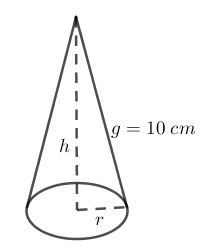
\includegraphics[width=.2\textwidth]{imagenes/imagenes05/T05IM17.png}
	\end{figure}
	
	\footnotesize{Pitágoras: $10^2=h^2+r^2 \to r^2=100-h^2$ (*)}
	
	\vspace{3mm}
	
	\normalsize{Volumen del cono: $V=\dfrac 1 3 \pi r^2 \; h =(*)= \dfrac \pi 3 (100-h^2)\; h= \dfrac \pi 3 (100h-h^3)$}
		
	\end{multicols}

	Para encontrar las dimensiones mínimas de la capacidad del cono, busquemos los $PC(V'): \to V'=\dfrac \pi 3 (100-3h^2)$. Los únicos puntos críticos pueden provenir, en esta ocasión, de $V'=0 \to h=+\sqrt{100/3} \approx 5.77 \; cm$. Obviamente hemos tomado la solución $h>0$ y se deja al al lector comprobar que se trata de un mínimo (por ejemplo, usando el criterio de la segunda derivada y comprobando que $V''(+\sqrt{100/3})<0$).
	
	Para esta $h=+\sqrt{100/3}$, calculamos por (*) el radio correspondiente, obteniendo $r=+\sqrt{200/3} \approx 8.16\; cm$. Con estos valores, el volumen mínimo del cono es $V=\dfrac {2000\pi}{9\sqrt{3}}\approx 403.07 \; cm^3$
	\end{proofw}
	
	\begin{ejre} Sean $a$ y $b$ dos números positivos cuyo producto es $a\cdot b=16$, ?`puede ser $a+b$ menor que 7?
		
	\end{ejre}
	
	\begin{proofw}\renewcommand{\qedsymbol}{$\diamond$}
	
	Como $a\cdot b=16 \to b=\dfrac {16}{a}$ (*). Construyamos la función suma  $S(x)=a+b=(*)=a+ \dfrac {16}{a}$, que es continua y derivable, $S'(a)=1-\dfrac {16}{a^2}$, en $]0,+\infty[$, ya que $a>0$. Asi que, los únicos $PC(S')$ los vamos a obtener de igualar $S'=0\to a=4$, pues $a>0$. Es fácil observar que para $0<a<4: \to  y'<0 \to y:\ \searrow$  y para $x>4: \to y'>0 \to y:\; \nearrow$. Luego hay un mínimo en $(4,S(4))=S(4,8)$ por lo que la suma de $a+b$ nunca puede ser menor a $7$ (de hecho, $8$ será su valor mínimo).
	
	\end{proofw}
	
	\begin{ejre} En un cuadrado de lado $10\; cm$ queremos apoyar un cilindro cuya área lateral sea de $50 \; cm^2$. ?`Cuál debe ser el radio del cilindro para que su volumen sea máximo?.
		
	\end{ejre}
	
	\begin{proofw}\renewcommand{\qedsymbol}{$\diamond$}
	
	Hagamos una figura que aclare el problema.
	
	\begin{multicols}{2}
	
	\begin{figure}[H]
	\centering
	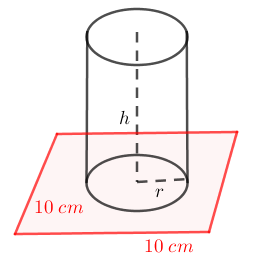
\includegraphics[width=.25\textwidth]{imagenes/imagenes05/T05IM18.png}
	\end{figure}
	
	$A_L: \quad  2\pi r h = 50 \to h=\dfrac {25}{\pi r}$ (*)
	
	$V_C: \quad V = \pi r^2 h = (*) = 25 r$
	
	$V'_C(r)=25 \to \nexists PC(V')$
	
	$V'>0, \; \forall r\in ]0,5] \to $ f siempre creciente
		
	\end{multicols}
	
	Luego $V$ alcanza el máximo para $r=5\; cm$ (diámetro $10\; cm$, lados del cuadrado donde se apoya y, para este $r$ se obtiene $(*):\; h=5 / \pi \approx 1.50\; cm$. El volumen máximo, para estas condiciones es $V=\pi \; 5^2\; dfrac {5}{\pi}= 125 \; cm^3 $  (Buscamos $M$ de $V$ en $r\in[0,5]$; un $M_{Abs}$, deberíamos tabular $V$ en $\{0,5\}$ pues no hay $PC(V')\in]0,5[$)
	
	\end{proofw}
	
	\begin{ejre} Dos postes de $12m$ y $18m$ de altura distan entre sí $30m$. Se desea tender un cable que una un punto del suelo entre los dos postes con los extremos de ambos. ?`Dónde hay que colocar el punto de anclaje en el suelo para que la longitud del cable sea mínima?
		
	\end{ejre}
	
	\begin{proofw}\renewcommand{\qedsymbol}{$\diamond$}
	
	
	\begin{multicols}{2}
	
	\begin{figure}[H]
	\centering
	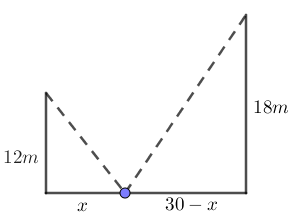
\includegraphics[width=.35\textwidth]{imagenes/imagenes05/T05IM19.png}
	\end{figure}
	
	\hspace{6mm}Pitágoras-1: $12^2=x^2+l_1^2$; 
	
	Pitágoras-2: $18^2=(30-x)^2+l_2^2$
	
	Longitud del cable: $L(x)=l_1+l_2$
	
	Abreviando: 
	
	$L(x)= \sqrt{x^2+144}+ \sqrt{x^2-60x+1224}$
		
	\end{multicols}
	
	A la búsqueda de los puntos crítico de $L'(x)$. Atención, $x\in [0,30]$ por las condiciones del problema.
	
	$L'(x)= \dfrac {2x}{2\sqrt{x^2+144}} + \dfrac {2x-60}{2\sqrt{x^2-60x+1224}}= $
	
	$=\dfrac {x\sqrt{x^2-60x+1224}+(x-30)\sqrt{x^2+144}}{\sqrt{x^2+144} \cdot \sqrt{x^2-60x+1224}}$
	
	$L'=0$ si lo es el numerador que es una ecuación irracional. Separando las raíces en los dos miembros de la ecuación y elevando al cuadrado se obtiene una ecuación de segundo grado cuyas soluciones son $x=12$ y $\cancel{x=-60}$ obviamente no aceptable.  Se deja al lector la comprobación de lo dicho.
	
	También se le deja el comprobar que para $x=12$, $L$ presenta un mínimo (estudiando el signo de $L'$ a la izqda. y dcha. de $x=12$)
	
	El punto de anclaje hay que situarlo a $12m$ del poste pequeño de $12m$ de alto y a $18m$ del poste grande de $18m$.
	
	\textcolor{gris}{Casualidad: pensad que se han obtenido dos triángulos isósceles.}
	
	\end{proofw}


	
	\begin{ejre} Se ha observado que en una carretera de salida de una gran ciudad la velocidad de los coches entre las 2 horas y las 6 horas de la tarde viene dada por: $v(t)=t^3-15t^2+72t+8$ para $t \in[2,6]; \quad t(h);\ v(km/h)$. ?`A qué hora circulan los coches con mayor y menor velocidad?
		
	\end{ejre}
	
	\begin{proofw}\renewcommand{\qedsymbol}{$\diamond$}
	
	Atención: nos piden que busquemos M y/o m en un intervalo cerrado, $[2,6]$, por lo que buscaremos los puntos críticos de $v'(t)$ en  $]2,6[$ y construiremos una tabla donde calcular $v(t)$ en estos puntos críticos y en los límites del intervalos $t=2\; \wedge \; t=6$.
	
	\begin{multicols}{2}

	$v'(t)=3t^2-30t+72 \to v'(t)= 0 \leftrightarrow x=4 \; \wedge \; x=6 $
	
	\begin{table}[H]
	\centering
	\begin{tabular}{|c|c|c|c|}
	\hline
	 $t(h)$& 2 & 4 & 6 \\ \hline
	$v(km/h)$ & 100 & 120 & 116 \\ \hline
	\end{tabular}
	\end{table}
	
	\end{multicols}
	
	La velocidad máxima, de $120 km/h$ se obtiene para $t=4h$ y la velocidad mínima de $100 km/h$ se obtiene para $t=2h$.
	
	\end{proofw}
	
	
	
	\begin{ejre} Descomponer el número
	81 en dos sumandos de forma que el producto del primer sumando por el cuadrado del segundo sea máximo.
	\end{ejre}
	
	\begin{proofw}\renewcommand{\qedsymbol}{$\diamond$}
	
	$81=x+y \to x=81-y (*); \quad P=x\cdot y^2=(*)=(81-y)y^2=81y^2-y^3$
	
	$P'(y)=162y-3y^2=3y(54-y)  \to  PC(P'):\; P'=0=3y(54-y) \to  y=0 \; \wedge \; y=54$
	
	Usaremos el criterio de la segunda derivada para averiguar si se trata de M o m cada uno de los resultados obtenidos, aunque en este, como en tantos otros problemas, el contexto es más que suficiente para decidir.
	
	$P''(y)=162-6y \ to \begin{cases}
 	y=0 \to P''(0)=162>0 \to y=0 \mbox{ mín.} \\
 	y=54 \to P''(54)=-162<0 \to y=54 \mbox{ máx.} 
	 \end{cases}$
	 
	 Soluciones: $y=0; \; x=81 \to P=0: \mbox{ mímimo;} \; y=54; \; x=27 \to P=1458 \; \mbox{máximo}$
	 
	\end{proofw}


	\begin{ejre} Una multinacional ha estimado que anualmente sus ingresos en euros vienen dados por la función: $I(x) = 28x^2 + 36000x$ , mientras que sus gastos (también en euros) pueden calcularse mediante la función $G(x) = 44x^2 + 12000x + 700000$, donde $x$ representa la cantidad de unidades vendidas.
	
	Determinar:
	\begin{enumerate}[a) ]

	\item La función que define el beneficio anual en euros.
	\item La cantidad de unidades que deben ser vendidas para que el beneficio sea máximo. Justificar que es máximo.
	\item El beneficio máximo.

	\end{enumerate}
	
	\vspace{-3mm}
	\textcolor{gris}{(este tipo de problemas de optimización suelen aparecer más en las matemáticas de las ciencias sociales)}
		
	\end{ejre}
	
	\begin{proofw}\renewcommand{\qedsymbol}{$\diamond$}
$B(x)=I(x)-G(x)=-16x^2 + 24000x - 700000 \to  B'(x)=-32x+24000 \to B'=0 \leftrightarrow x=750\;$ artículos. Se deja al lector comprobar que efectivamente se trata de una máximo y que los beneficios máximos ascenderán a  $8300000 $ euros.
	
	\end{proofw}
	
\vspace{7mm}
	
	\begin{ejre}  Problema del ogro.
	\begin{multicols}{2}

	$\divideontimes$ Todos los días debes recorrer la distancia desde A hasta B, que es de 2u. El 50. $\%$ de las veces aparece, a mitad del camino, un ogro que crea una muralla infranqueable, centrada en el camino, también de 2 u. Averigua cuál es el camino que minimiza la distancia media a recorrer para ir desde A hasta B.

	\begin{figure}[H]
	\centering
	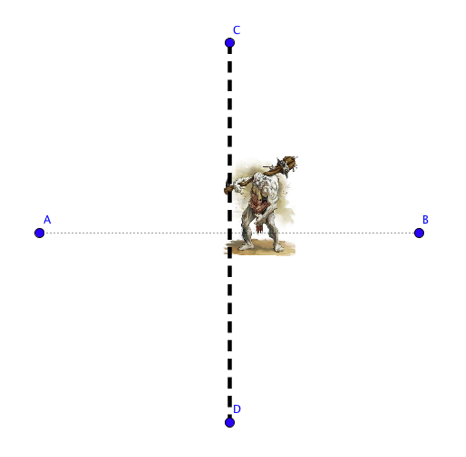
\includegraphics[width=.4\textwidth]{imagenes/imagenes05/T05IM20.png}
	\end{figure}
	\end{multicols}
	
	
	\end{ejre}
	
	\begin{proofw}\renewcommand{\qedsymbol}{$\diamond$}
	
	\begin{multicols}{2}
	
	\begin{figure}[H]
	\centering
	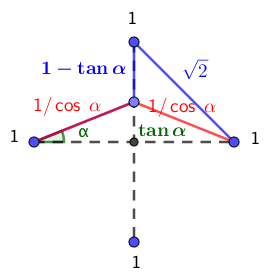
\includegraphics[width=.35\textwidth]{imagenes/imagenes05/T05IM21.png}
	\end{figure}
	
	\small{Nos dirigiremos todos los días hacia la barrera con un ángulo $\alpha$. Si no está el ogro (el $50\%$ de las veces, $n/2$,  cruzaremos la barrera hasta el punto B. A esta trayectoria la llamaremos \textcolor{roig}{$l_1$}. La otra mitad de las veces $n/2$, al encontrarnos con el ogro, subiremos toda la barrera y, desde allí, iremos a nuestro destino que se encuentra a $\sqrt{2}\; u$ de distancia, llamaremos a esta trayectoria \textcolor{blau}{$l_2$}.}
		
	\end{multicols}

\normalsize{La longitud media que recorreremos es}: 

$L_M=\frac n 2 \textcolor{roig}{l_1}+\frac n 2 \textcolor{blau}{l_2}$: $\qquad l_1= \dfrac {1}{\cos \alpha} + \dfrac {1}{\cos \alpha} =\dfrac {2}{\cos \alpha} ; \quad l_2=\dfrac {1}{\cos \alpha} +1-\tan \alpha + \sqrt{2}$
	
	$ L_M=\frac n 2 l_1 + \frac n 2 l_2= \frac n 2  \left[ \dfrac {3}{2 \cos \alpha} + \dfrac {1} {2} \tan \alpha+ \dfrac {\sqrt{2}+1}{2} \right] \Rightarrow$
	
	$\Rightarrow L'=\frac n 2 \left[ \dfrac {3 \sin \alpha}{2 \cos^2 \alpha} - \dfrac {1}{2 \cos^2 \alpha} \right]; \qquad $ como $\cos \alpha \neq 0; (\alpha = 90^o$ no tendría sentido, necesariamente (para los $PC(L_M')$), ha de ocurrir que $L_M'(\alpha)=0 \to \sin \alpha = 1/3 \to \alpha\approx19.5^o$. El punto al que nos debemos dirigir en todas las ocasiones, para minimizar nuestro trayecto, es a $19.5^o$ del centro de la muralla.
	
	\end{proofw}
	
	\begin{ejre} Dentro de una cartulina rectangular se desea hacer un dibujo que ocupe un rectángulo $R$ de $600 cm^2$de área de manera que:
	

		Por encima y por debajo de R deben quedar unos márgenes de $3 cm$ de altura cada uno. Los márgenes izquierda y derecha de R deben tener una anchura de $2 cm$ cada uno.
		
	Obtener razonadamente:
	
	
 	$\quad a)\; $ El área de la cartulina en función de la base $x$ del rectángulo $R$.
 	
 
 	 
 	 $\quad b)\; $El valor de $x$ para el cual el área de la cartulina es mínima. 
 	
 	$\quad c)\; $Las dimensiones de dicha cartulina de área mínima.
	 
	 
	  	
	\end{ejre}

	\begin{proofw}\renewcommand{\qedsymbol}{$\diamond$}
	
	De nuevo, necesitamos de una figura.
	
	\begin{multicols}{2}
	\begin{figure}[H]
	\centering
	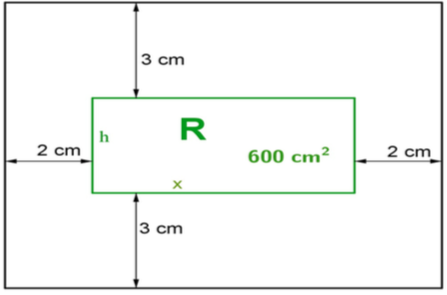
\includegraphics[width=.4\textwidth]{imagenes/imagenes05/T05IM22.png}
	\end{figure}
	
	$x\; h=600 \to h=\dfrac {600} x; \; x>0$ (*)
	
	Las medidas de la cartulina son: $base=x+4; \; altura=h+6$
	
	Y el Área: $A=base\cdot altura= (x+4)(h+6)=(*)=(x+4)\left(\dfrac {600}{x}+6\right)= 624+6x+\dfrac {2400}{x}$.
	
		
	\end{multicols}

	Para el área mínima: $A'= 6-\dfrac{2400}{x^2}$, que como $x>0$, para buscar los $PC(A')$ haremos $A'=0 \to x=+20$ (solo aceptamos la solución positiva).
	
	Se deja al lector comprobar que se $x=20cm$ trata de un mínimo y que la cartulina tiene la base de $24cm$ y la altura de $36cm$, siendo el área mínima de $864cm^2$.
	\end{proofw}

	\begin{ejre} Un proyectil está unido al punto $(0, 2)$ por una cuerda elástica y tensa. El proyectil recorre la curva $y = 4 -x^2$ de extremos $( -2, 0)$ y $(2, 0)$. Obtener razonadamente:

	$\quad a)\; $ La función de la variable $x$ que expresa la distancia entre un punto cualquiera $(x, 4 -x^2)$ de la curva $y=4-x^2$ y el punto $(0,2)$. 
	
	$\quad b)\; $ Los puntos de la curva $y = 4 -x^2$ para $ - 2 \le  x \le  2$ que se encuentren a mayor y menor distancias absolutas del punto $(0,2)$. 
	\end{ejre}
	
	\begin{proofw}\renewcommand{\qedsymbol}{$\diamond$}

	El vértice de la parábola esta en $V(0,4)$ y corta al eje $OX$ en los puntos $(\pm 2, 0)$
	
	$d\left( (0,2); (x,4-x^2)  \right)= +\sqrt{x^2+(2-(4-x^2))}=\sqrt {x^4-3x^2+4}; \quad -2\le x \le 2$
	 
	 $d'=\dfrac {4x^3-6x^2}{2 \sqrt {x^4-3x^2+4}}$
	 
	 Como el denominador $2d\neq 0$, pues $d\neq 0$ en -$2\le x \le 2$. Necesariamente, $PC(d') \to d'=0$
	
	\begin{multicols}{2}

	$d'=0 \to 2x(2x^2-3)=0 \leftrightarrow x=0 \; x=\pm \sqrt{6}/2$. Como buscamos M.m en un intervalo cerrado $[-2,2]$, buscamos M, m Absolutos y hemos de tabular la función $d$ en $\{\pm 2; \; \pm \sqrt{6}/2; \; 0 \}$
	
	\begin{figure}[H]
	\centering
	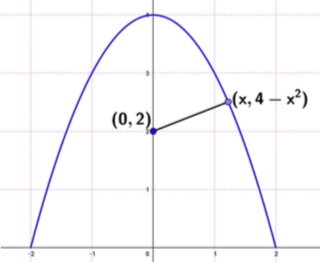
\includegraphics[width=.3\textwidth]{imagenes/imagenes05/T05IM23.png}
	\end{figure}
	
	\end{multicols}
	
	
	
		
	\begin{table}[H]
	\centering
	\begin{tabular}{|c|c|c|c|c|c|}
	\hline
	 x& -2 & $-\sqrt{6}/2$ & 0 & $\sqrt{6}/2$ & 2 \\ \hline
 	d&  2.83& 1.32 & 2 & 1.32 & 2.83 \\ \hline
	\end{tabular}
	\end{table}	
		
	
	

	
	La distancia máxima absoluta es de 2.83 u y se encuentra en dos puntos $(\pm2,0)$. 	La distancia mínima es de 1.32 y y también se alcanza en dos puntos $(\pm \sqrt{6}/2, 5/2)$
	
	\end{proofw}

	\begin{ejre} Se desea construir un campo rectangular con vértices A, B, C y D de manera que: los vértices A y B sean puntos del arco de la parábola $y=4-x^2$; $\; -2\le x\le 2\; $, y el segmento de extremos A y B es horizontal. Los vértices C y D sean puntos del arco de la parábola $y=x^2-16\; $,$\; -4\le x\le 4$, y el segmento de extremos C y  D es horizontal.Los puntos A y C deben tener la misma abcisa, cuyo valor es el número real positivo $x$Los puntos B y D deben tener la misma abcisa, cuyo valor es el número real negativo $-x$. Se pide obtener razonadamente:
 
	$\quad a) \; $ La expresión $S(x)$ del área del campo rectangular en función del número real positivo $x$. 
	
	$\quad b) \; $ El número real positivo $x$ para el que el área $S(x)$ es máxima.  
	
	$\quad c) \;$ El valor del área máxima	
	
	\end{ejre}

	\begin{proofw}\renewcommand{\qedsymbol}{$\diamond$}
	
	
	Necesitamos una figura (por construcción, $x \in ]0,2]$:
	\begin{multicols}{2}
	
	
	\begin{figure}[H]
	\centering
	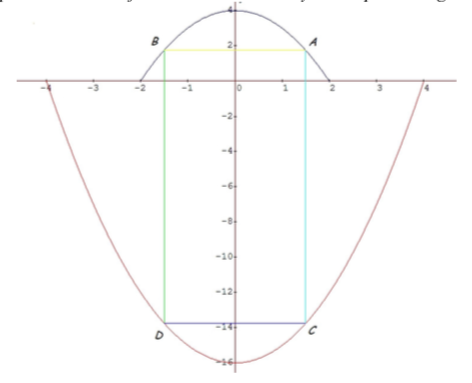
\includegraphics[width=.4\textwidth]{imagenes/imagenes05/T05IM24.png}
	\end{figure}
	 $A(x, 4-x^2); \; B(-x, 4-x^2)$
	 
	 $C(x,x^2-16); \; D(-x, x^2-16)$
	 
	 base rectángulo: $2x$
	 
	 altura rectángulo; $4-x^2-(x^2-16)=20-2x^2$
	 
	 área: $S(x)=2x(20-2x^2)=40x-4x^3; \;  x \in ]0,2]$
	 
	 $s'(x)=40-12x^2$, como $\nexists x\; / \; \nexists S'$, necesariamente $PC(S'): \; S'=0\to x=+\sqrt {10/3} \; \in ]0,2]$
	 
	\end{multicols}

	 Se deja al lector comprobar que esta es la solución que conduce a un área máxima $S_{max}=\frac {80}3	\frac {\sqrt{10}} 3 \approx 48.69\; u^2$
	\end{proofw}
	
	\begin{ejre} A las 7 de la mañana, una lancha A está situada a $150 km$ al este de otra lancha B. La lancha A navega hacia el oeste a una velocidad constante de $40 km/h$ y la lancha B se dirige hacia el norte a $30 km/h$. Si se mantienen estos rumbos, averiguar razonadamente a qué hora estarán ambas lanchas a distancia mínima.	
	\end{ejre}

	\begin{proofw}\renewcommand{\qedsymbol}{$\diamond$}	
	
	Necesitaremos un dibujo para resolver este problema.
	\begin{multicols}{2}
	$d(t)=+\sqrt{(30t)^2+(150-40t)^2}=$
	
	$=\sqrt{2500t^2-12000t+22500}$
	
	$=10\sqrt{25t^2-120t+225}	$
	

	
	$d'(t)=10 \dfrac {50t-120}{2\sqrt{25t^2-120t+225}}$ 	
	\begin{figure}[H]
	\centering
	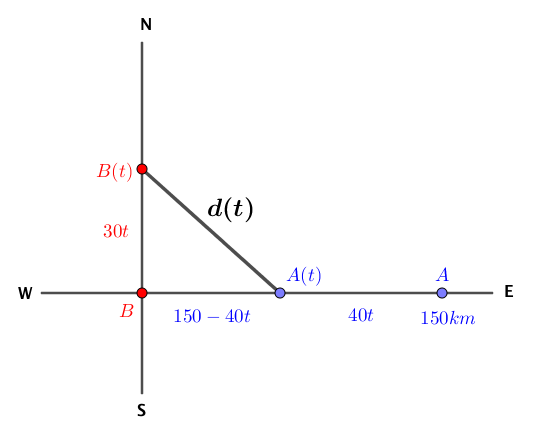
\includegraphics[width=.45\textwidth]{imagenes/imagenes05/T05IM25.png}
	\end{figure}
	\end{multicols}	
	Como el denominador no puede ser cero (crompruébelo el lector), los únicos $PC(d')$ provendrán de $d'=0=50t-120 \to t=2.4\; h$, que también se deja al lector el comprobar que es un mínimo (recuérdese que, por las condiciones del problema, $t\in[0,\infty]$).

	La distancia mínima ocurre a las $2.4\; h$ de que empiecen a moverse las lanchas, es decir, a las $7+2.4=9.4=9\; h \; 24\; min$. Calcule el lector la distancia mínima en $km$ a que se encuentran las lanchas sin más que sustitutir $t=2.4$ en la ecuación que da la distancia entre barcas $d(t)$
	
	\end{proofw}

	

\subsection{Ejercicios propuestos de aplicaciones de las derivadas}

	\underline{Rectas tangente y Normal.}

	\begin{enumerate}
		\item Un vehículo espacial despega de un planeta con una trayectoria dada por $y=30x-0.5x^2\; (x \mbox{ e } y \mbox { en } km)$. La dirección del vehículo nos la proporciona la recta tangente en cada punto. Determina la dirección del vehículo cuando está a $4\; km$ sobre el horizonte.
		 
		\rightline{\textcolor{gris}{Solución: supondremos que los $4\; km$ sobre el horizonte }}
		\rightline{\textcolor{gris}{son en la dirección horizontal: $x=4\; km$}}
		\rightline{\textcolor{gris}{ $RT(x=4):\; y=26x+8 ; \; m=8 \tan \theta \to \theta=87.9^o$}}
		
		\item Determina los puntos de la gráfica $y=x^3-3x+2$ en los que su tangente sea paralela a las rectas $\quad a) \; y=0; \quad b)\; y=2x$
		
		\rightline{\textcolor{gris}{Solución: $a)\; x=\pm 1\quad b)\; x=\pm \sqrt{5/3}$}} 
		
		\item Determina las rectas tangentes a la función $y=4x^3-12x$ en los puntos en que la pendiente es 12. ?`Cuál es el menor valor que puede tener la pendiente a esta curva? ?`En qué puntos se alcanza?
		
		\rightline{\textcolor{gris}{Solución: $m=12 \leftarrow x=\pm1;$}}
		\rightline{\textcolor{gris}{ $m(x)=f'(x) \mbox{ tiene un mínimo en } x=0 \mbox{ y } m(0)=f'(0)=0$}}
		
		\item Determina los coeficientes $a$, $b$ y $c$ de la función $f(x)=ax^3+bx+c$, que pase por el punto $A(1,2)$ y sea $y=x$ su recta tangente en $O(0,0)$.
		
		\rightline{\textcolor{gris}{Ayuda: Pase $(1,2)\to x=1; y=2; \;$ pase $(0,0) \to x=0); \; y=0\; y=x$}}
		 \rightline{\textcolor{gris}{$y=x \; RT$ en  $x=0 \to f'(0)=1 \quad   \to \quad \Rightarrow \;  a=-1/2; \; b=3/2; \; c=0$}}
		
		\item Encuentra la ecuación de las rectas tangentes a las funciones el los puntos que se indican:
		
		\begin{multicols}{2}
		\begin{enumerate}[a) ]	
		\item $y=\ln(\tan 2x)\; $ en $x=\pi/8$
		\item $y=\sqrt{\sin 5x}\; $ en $x=\pi/6$
		\item $x^2+y^2-2x-8y+15=0\; $ en $x=2$
		\item $y=(x^2+1)^{\sin x}\; $ en $x=0$
		\end{enumerate}
		\end{multicols}
 
		\rightline{\textcolor{gris}{Solución: $a)\; y=4x-\pi/2; \quad b)\; y-\sqrt{2}/2=-5\sqrt{6}/4\cdot (x-\pi/6)$}} 
		\rightline{\textcolor{gris}{$c) \; y=-x+7 \; \wedge \; y=x+1; \quad d)\; y=1$}}
		
		\item Halla un punto de la gráfica de la función $y=2\sqrt{x}$ en el que la tangente forme un ángulo de $60^o$ con el eje $X$. Escribe la ecuación de la recta tangente.
		
		\rightline{\textcolor{gris}{Solución: $(1/3,2\sqrt{3}/3; \; RT:\; y=\sqrt{3}x+\sqrt{3}/3$}} 
		
		\item Encuentra ls puntos de la curva $y=3x^2-5x+12$ en los que la recta tangente pase por el origen de coordenadas.
		
		\rightline{\textcolor{gris}{Solución: $y=-17x; \;  y=7x$}} 
		
		\item Encuentra la ecuación de la RT a $y=x^3+3x^2-5$ que sea perpendicular a la recta $2x+6y+1=0$
		
		\rightline{\textcolor{gris}{Solución: $3x+y+6=0$}}
		
		\item Encuentra la ecuación normal a la parábola $y=x^2-6x+2$ perpendicular a la recta que une el origen de coordenadas con el vértice de la parábola.
		
		\rightline{\textcolor{gris}{Solución: $4x-4y-21=0$}}
		
		\item Encuentra la normal a la curva $y=x\ln x$ que sea paralela a la recta $2x-2y+3=0$
		
		\rightline{\textcolor{gris}{Solución: $x-y-3e^{-2}=0$}}
		
		\item Encuentra la RT a $x^2(x+y)=a^2(x-y)$ en el origen de coordenadas.
		
		\rightline{\textcolor{gris}{Solución: $y=x$}}
		
		\item Encuentra las RT a $y^2+4x=0$ que pase por $P(2,1)$.
		
		\rightline{\textcolor{gris}{Solución: $x+2y-4=0;\; \; x-y-1=0$}}
		
		\item Encuentra la ecuación de las recta normal a la hipérbola $4x^2-y^2=36$, que sean paralelas a la recta $2x+5y-4=0$.
	
		\rightline{\textcolor{gris}{Solución: $2x+5y-50=0; \; \; 2x+5y+50=0$}}
		
		
	\underline{Máximos mínimos. Puntos de inflexión.}
	
		\item Encuentra el ángulo que forman las rectas tangentes a la función $y=x^4-6x^2$ trazadas en sus puntos de inflexión.
		
		\rightline{\textcolor{gris}{Solución: $14.83^o$}}
		
		\item Estudia Los extremos relativos de $f(x)=0.4x^5+0.5x^4-4x^3$. ?`$x=0$ es M o m?
		
		\rightline{\textcolor{gris}{Solución: $M(-3,51.3); \; I(0,0); \; m(3,-11.2)$}}
		
		\item En un experimento, la cantidad de agua en función del tiempo viene dada por la función $C(t)=\dfrac 2 3 + 10t+ \dfrac {10}{t}+\dfrac {240}{t^3}$, con $t\in [1,10]\; $, $t(h)\; $ y $\; C(l)$. Calcula cuál es la cantidad mínima de agua y en que momento se obtiene.
		
		\rightline{\textcolor{gris}{Solución: \scriptsize{Ayuda, se trata de M.m Absolutos} (intervlo cerrado): $m(3,C(3))=m(3\; h; 43.9\; l)$}}
		
		\item Calcula los extremos absolutos de $f(x)=\ln (x^2+1) + (x-3) $ en el intervalo $[-2,3]$
		
		\rightline{\textcolor{gris}{Solución: $m_A(-2, \ln5 - 5); \; M_A(3,\ln 10)$}}
		
		\item Estudia la monotonía y extremos de la función: $y=(x-1)^4 (x+1)^2 (x-3)$.
		
		\rightline{\textcolor{gris}{Solución:$M(-1,0);\; m(-3.76,-4.7); \; M(1,0); \; m(12.15,-12)$}}
		
		\item Estudia la monotonía y extremos de la función: $y=|x^3|+\dfrac 3 x$.
		
		\rightline{\textcolor{gris}{Solución: $m(1,4); \ x=0 \mbox{ discont. asint.}$}}
		
		
		\item Encuentra los extremos relativos de las funciones:
		
		\begin{multicols}{2}
		\begin{enumerate}[a) ]
		\item $y=\dfrac{x^2-5x+4}{x^2+5x+4}$
		\item $y=\dfrac x 3 - \sqrt[3]{x}$
		\item $y= \arctan \left(\dfrac {x}{1+x^2} \right)$
		\item $y= \dfrac {x^3}{e^{x^2}}$
		\item $y= x^3-3\ln x + 2$
		\item $y= |x|+\dfrac {4}{x-5}$
		\end{enumerate}	
		\end{multicols}

		
		\rightline{\textcolor{gris}{Solución: a) M en -2 y m en 2; b) M en -1; m en 1; c) m en -1; M en 1}}
		
		\rightline{\textcolor{gris}{d) m en $-\sqrt{3}/2$; M  en $\sqrt{3}/2$; e) m en 1; f) m en 0; M en 3; m en 7}}
		
		\item Encuentra las relaciones que han de cumplir los coeficientes de un polinomio general de $4^o$ grado para que tenga $2$, $1$ o ningún punto de inflexión.
		
		\rightline{\textcolor{gris}{Solución:$y=ax^4+bx^3+cx^2+d^x+e$}}
		\rightline{\textcolor{gris}{2 PI: $\; 3a^2>bc; \quad$; 1 PI: $\; 3a^2=bc; \quad$ Ningún PI: $;\ 3a^2<bc; \quad \forall d,\; e$}}
		
		\item Calcula $p$ y $q$ para que la función $f(x)=\dfrac {x^2+px+q}{x}$ Tenga un máximo igual a $-1$ y un mínimo igual a $1$. 
		
		\rightline{\textcolor{gris}{Solución: $p=0; \; q=1/4$}}
		
		\item Sea $f(x)=\dfrac {ax^2+1}{a+x}$, tiene un extremo relativo en $x=1$. Determina el valor de $a$. 
		
		\rightline{\textcolor{gris}{Solución: $a=1/2$}}
		
		\item Para la función $f(x)=\dfrac {3x^2-5x+5}{2x^2-3x+4}$, comprueba que es continua y que $\underset {x\to \pm \infty}{lim}\;{f(x)}=3/2$. Estudiando sus intervalos de monotonía, determina entre qué números toma todos sus valores.
		
		\rightline{\textcolor{gris}{Solución: $f(x) \subset [1, 35/23]$}}
		
		\item $\divideontimes$ Encuentra los intervalos de monotonía de la función $y=x+|\sin x|$.
		
		\rightline{\textcolor{gris}{Solución: Creciente en todo $\mathbb R$}}
		
		\item $\divideontimes$ Encuentra los intervalos de monotonía de $y=x\; \sin (\ln (x))$ \textcolor{gris}{Cuidado con el dominio}.
		
		\rightline{\textcolor{gris}{Solución: m en $x=e^{\dfrac {3\pi}{4}+2k\pi}$; M en $ x=e^{\dfrac {3\pi}{4}+2(k+1)\pi} \quad \forall k \in \mathbb N$ }}

		
	
	\underline{Problemas de OPTIMIZACIÓN.}
		
		\item Hallar los puntos de la parábola $y=x^2-1$ que se encuentre a una distancia mínima del punto $A(-2,-1/2)$
		
		\rightline{\textcolor{gris}{Solución: $m(-1,0)$}}
		
		\item Encuentra las dimensiones del rectángulo de mayor área inscrito en una circunferencia de radio $R$
		
		\rightline{\textcolor{gris}{Solución: $x=y=\sqrt{2}\; R; \quad S=\sqrt{2}R \cdot \sqrt{2}R= 2 R^2$}}
		
		\item Encuentra los puntos de la curva $y=\dfrac {1}{1+x^2}$ (`curva de Agnesi') en que la recta tangente tiene pendiente máxima y determina el valor de esa pendiente.
		
		\rightline{\textcolor{gris}{Solución: El punto es $(-\sqrt{3}/3,3/4); \quad $  la pendiente máxima es   $3\sqrt{3}/8$}}
		
		\item Se va a construir un depósito de $1500 m^3$ de capacidad, con forma de caja abierta por la parte superior. Su base es un cuadrado y las paredes laterales son cuatro rectángulos iguales perpendiculares a la base. El precio de cada $m^2$ de la base es de $15$ euros y el precio de cada $m^2$ de pared lateral es de $5$ euros.
		
	Obtener, razonadamente, el coste total del depósito en función de la longitud $x$ de un lado de la base, así como las longitudes del lado de la base y de la altura del depósito para que dicho coste total sea mínimo. ¿Cuál es este coste mínimo? 	
	
	
		\rightline{\textcolor{gris}{Solucción $C(x)=15x^2+\dfrac {3000}{x}; \; x\in \mathbb R^+ \quad x_m=10m; \; y_m=15m; \; C_m=4500\; $ euros. }}
		
		
		
		
		
		\item  Se considera el triángulo $T$ de vértices $O = (0, 0)$ , $A = (x, y)$ y $B = (0, y)$, siendo $x>0,\;y>0$ , y tal que la suma de las longitudes de los lados $\overline{OA}$ y $\overline{AB}$ es $30m$.
		 
		Obtener razonadamente el área del triángulo $T$ en función de $x$, el valor de $x$ para el que dicha área es máxima y el valor de dicha área máxima.
		
		\rightline{\textcolor{gris}{Solución:$A_T=\dfrac {x\sqrt{900-60x}}{2}; \; 0<x<15; \quad x_M=10m; \quad A_M=86.6025m^2$}}
		
		\item Se estudió el movimiento de un meteorito del sistema solar durante un mes. 
		
		
		Se obtuvo que la ecuación de la trayectoria $T$
		es $y^2=2x+9$, siendo $-4.5\le x \le 8$ e $y \ge 0$, estando situado el Sol en el punto $(0,0)$. Obtener razonadamente:
		
	$\quad a)\; $ La distancia del meteorito al Sol desde un punto $P$ de su trayectoria cuya abcisa es $x$.

	$\quad b)\; $ El punto P de la trayectoria $T$ donde el meteorito alcanza la distancia mínima al Sol. 
	
	$\quad c)\; $ Distancia minima del meteorito al Sol.

		
		\rightline{\textcolor{gris}{Solución:$d(P,\odot)=\sqrt{x^2+2x+9}; \; -4.4\le x \le 8; \quad x_m=1\; u; \quad d_{min}=\sqrt{8}\; u$}}
		
		\item Se tiene un cuadrado de mármol de lado $80 cm$. Se produce la rotura de una esquina y queda un pentágono de vértices $A = (0, 20)$, $B = (20, 0)$, $C = (80, 0)$, $D = (80, 80)$ y $E = (0, 80)$. Para obtener una pieza rectangular se elige un punto $P = (x , y)$ del segmento $\overline{AB}$ y se hacen dos cortes paralelos a los ejes $X$ e $Y$. Así se obtiene un rectángulo cuyos vértices son los puntos $P=(x,y),\; F=(80,y),\;  D=(80,80), \;  G=(x,80)$.
		Obtener razonadamente, el valor de $x$ para el que el área del rectángulo $R$ es máxima y el valor de esa área.
		
		\rightline{\textcolor{gris}{Solución: $x=10cm; \; A=4900cm^2$}}
		
		\item Se divide un alambre de longitud $100 cm$ en dos partes. Con una de ellas, de longitud $x$, se construye un triángulo equilátero y con la otra, de longitud $100 - x$, se construye un cuadrado. 
		?`Cual ha de ser el valor de $x$ para que la suma de las áreas de ambas figuras sea mínima?. ?`Y para que sea máxima? 
		\textcolor{gris}{Nota: recuérdese que buscamos M y m Absolutos en $x\in [0,100]$}
		
		\rightline{\textcolor{gris}{Solución: $x_m=56,5cm;\; A_m=182.4cm^2; \quad x_M=0cm; \; A_M=625$}}
		
		 \rightline{\textcolor{gris} {Para el máximo, todo el alambre se usa para construir un cuadrado de lado $25cm$}}
				
\end{enumerate}

\vspace{-5mm}

\section{Teoremas relativos a funciones derivables}

	
	\subsection{Teorema de Rolle}
	
	No siempre es fácil hallar los puntos críticos de una función. El teorema de Rolle indica las condiciones suficientes para que una función presente puntos críticos en un intervalo.
	
	
	\begin{teor} TEOREMA DE ROLLE: $f(x)$ continua en $[a,b]$ y derivable en $]a,b[$, tal que $f(a)=f(b)$  (tome valores iguales en los extremos) $\Rightarrow$ existe, al menos, un $c\in]a,b[$ tal que $f'(c)=0$
	\end{teor}
		

	\begin{proof}: 
	\begin{multicols}{2}
	
	Por el teorema de Weierstrass de funciones continuas en intervalos cerrados, existen, al menos $ x_M , \; x_m \; \in [a,b] $ donde $f(x)$  alcanza el máximo y en mínimo absolutos.
	
	Si $x_M$ o $x_m \; \in ]a,b[$, a ese punto le llamamos $c$ del teorema y ya hemos encontrado el punto crítico enunciado por Rolle, pues al ser $f$ derivable, $f'(c)=0$.
	
	Si ni $x_M$ ni $x_m$ pertenecen a $]a,b[\to $ necesariamente $x_M=a, \; x_m=b$ o al revés. Tanto da, el máximo absoluto y el mínimo absoluto se alcanzarían en los límites $a$ y $b$ del intervalo, pero como por hipótesis, $f(a)=f(b)$, necesariamente $f(x)=cte \to f'(x)=0, \; \forall x=c\in]a,b[$ y el teorema también quedaría demostrado. 
	
	\begin{figure}[H]
		\centering
		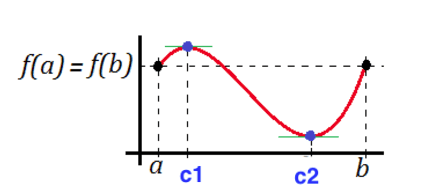
\includegraphics[width=0.5\textwidth]{imagenes/imagenes05/T05IM27.png}
		\caption {Teorema Rolle}	
	\end{figure}
	\end{multicols}
	\end{proof}
	
	
	
	NOTA: Las tres hipótesis del teorema de Rolle son no-redundantes, es decir, con que falle una sola de ellas no se puede aplicar el teorema.
 	\begin{figure}[H]
		\centering
		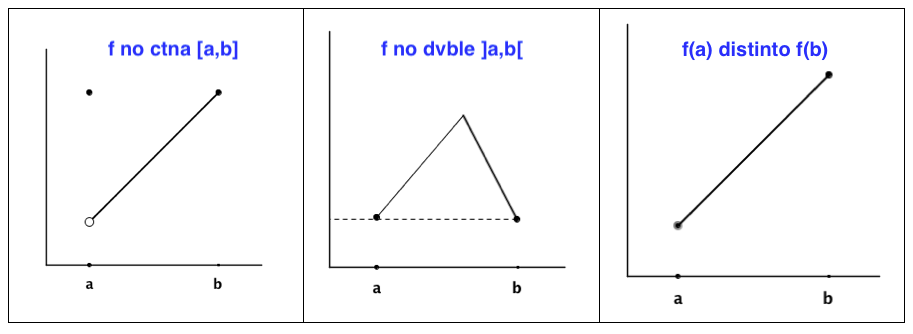
\includegraphics[width=0.9\textwidth]{imagenes/imagenes05/T05IM26.png}
		%\caption {Las hipótesis del T. Rolle son no-redundantes.}
	\end{figure}
	
	
	\subsection{Teorema del Valor Medio (TVM), de los incrementos finitos o de Bonet-Lagrange}
	
	\begin{teor}   $f(x)$ continua en $[a,b]$ y derivable en $]a,b[$, existe, al menos, un punto  $c\in ]a,b[$, donde la recta tangente en $(c(f(c))$ es paralela a la recta secante que une los extremos de la curva en el intervalo cerrado: $(a,f(a)); \; (b,(f(b))$.
	
	Es decir: $f \; ctna\;  [a,b]\; \wedge \; f \; dvble \;  ]a,b[ \; \Rightarrow \exists \; c\in \; ]a,b[\; : \quad f'(c)=\dfrac {f(b)-f(a)}{b-a}$
		
	\end{teor}
	
	\begin{proof}
		La recta secante que pasa por los puntos  $(a,f(a)); \; (b,(f(b))$ tiene por pendiente $m_{sec}=\dfrac {f(b)-f(a)}{b-a}$ y como pasa por $(a,f(a))$, su ecuación es: $r_{sec}:\; y-f(a)= \dfrac {f(b)-f(a)}{b-a} \cdot (x-a)$. Llamamos a esta recta, con la $y$ despejada, función $g(x)=y=f(a)+ \dfrac {f(b)-f(a)}{b-a} \cdot (x-a)$
		
		%\clearpage
		
		\begin{multicols}{2} 
		
		Es sencillo comprobar ahora, se deja como ejercicio al lector, que si construimos una nueva función 
		
		$h(x)=f(x)-g(x)=$
		
		$f(x)-f(a)- \dfrac {f(b)-f(a)}{b-a} \cdot (x-a)$, 
		
		cumple las tres hipótesis exigidas en el teorema de Rolle, por lo que 
		
		$\exists \; c\in]a,b[ \quad / \; h'(c)=0$, 
		
		de lo que se deriva, inmediatamente, la tesis del TVM.
		
		\begin{figure}[H]
		\centering
		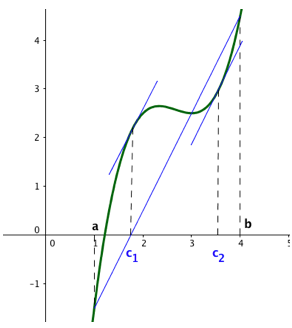
\includegraphics[width=0.4\textwidth]{imagenes/imagenes05/T05IM28.png}
		\caption {Teorema Valor Medio.}
		\end{figure}
		\end{multicols}
		
		\end{proof}
		
		\vspace{-3mm}
		
		En toda función ctna. dvble en in $I$, se puede trazar, al menos en un punto del abierto de $I$ una recta tangente que sea paralela al segmento que une los extremos de la curva en $I$
	
	\subsection{Teorema de Cauchy o del valor medio generalizado $\; \divideontimes$}
	
	\begin{teor}
	\label{ThCauchy}
	$f(x) \;  \wedge \; g(x) \; ctnas\;  [a,b]\; \wedge \;  dvbles \;  ]a,b[ \; $. Entonces existe al menos un punto $c\; \in\; ]a,b[$, tal que:
	$\left(f(b)-f(a) \right)\; g'(c)= \left(g(b)-g(a) \right)\; f'(c)$
	
	En el caso en que $g(b) \neq g(a) \; \wedge \; g'(c)\neq 0$, entonces se puede escribir:
	$\dfrac{f'(c)}{g'(c)} = \dfrac {f(b)-f(a)}{g(b)-g(a)}$
	
	\end{teor}
	
	\begin{proof}
	Definimos $h(x)=(g(b)-g(a)) \cdot (f(x)-f(a)) - (f(b)-f(a)) \cdot (g(x)-g(a))$
	
	Como $f(x)$ y $g(x)$ son ctnas. en $[a,b]$ y dvbles. en $]a,b[$, es fácil comprobar que $h(a)=h(b)$ y la función $h(x)$ cumple las tres hipótesis del th. de Rolle en $[a,b]$. Luego, existe un $c\; \in ]a,b[ \; / \; h'(c)=0$
	
	Derivando: $h'(c)=(g(b)-g(a)) \cdot f'(x) - (f(b)-f(a)) \cdot g'(x)$. Como $h'(c)=0 \to $
	
	$\to 0=(g(b)-g(a)) \cdot f'(c) - (f(b)-f(a)) \cdot g'(c)$
	
	De donde se deduce: $\left(f(b)-f(a) \right)\; g'(c)= \left(g(b)-g(a) \right)\; f'(c)$
	
	Si $g(b)-g(a)\neq 0 \; \wedge \; g'(c)\neq 0 \to$
	
	$\dfrac{f'(c)}{g'(c)} = \dfrac {f(b)-f(a)}{g(b)-g(a)}$ 
	
	\end{proof}
	El Th. de Cauchy se usa para la demostración de otros teoremas, p.e., la regla de L'Hôpital y el Th. de Taylor que veremos en el próximo tema.
	
	\subsection {Corolarios}
	\begin{coro}  
		$f(x) \;   ctna\; [a,b] \;  \wedge \;  dvble \;  ]a,b[ \; / \; f'(x)=0, \; \forall x\; \in ]a,b[ \; \Rightarrow \; f(x)$ es constante en todo $[a,b]$
	\end{coro}
	
	\begin{proof}
		Sea $a+h\; \in\;  ]a,b[ \to $ (th. \ref{teor:conserva-signo} conserv. signo límite) $f(a+h)-f(a)=f'(c)\cdot h$ Por hipótesis $f'(c)=0\to f(a+h)-f(a)=0 \to f(a+h)=f(a);\; \forall a+h\; \in \; ]a,b[ $ Luego, $f$ constante en $[a,b]$.
	\end{proof}

	\begin{coro} `Teorema fundamental del cálculo integral': 
	\label{teor:fdmtalCI}
		
		$f(x) \;  \wedge \; g(x) \; ctnas\;  [a,b]\; \wedge \;  dvbles \;  ]a,b[ \; $, si $f'(x)=g'(x); \; \forall \;x\; \in \,]a,b[ \; \Rightarrow \; f(x)-g(x)\;  $,  es una función constante en $[a,b]$.
		
	\end{coro}
	
	\begin{proof}
	Basta con aplicar el teorema anterior a la función $h(x)=f(x)-g(x)$.	
	\end{proof}


	
	\subsection{Regla de L'Hôpital}
	
	\begin{teor} $\divideontimes$ Teorema de L'Hôpital.
	
	$f(x)$ y $g(x)$ continuas y tales que $f(a)=0\; $ ó $(\infty)$  y $g(a)=0\; $ ó $(\infty)$. Entonces:
	
	$\underset {x\to a}{lim}\; {\dfrac {f(x)}{g(x)}}= \underset {x \to a}{lim}\; {\dfrac {f'(x)}{g'(x)}}$

	\end{teor}
	
	 El teorema también se verifica si $x\to a^{\pm} $ o $x\to \pm \infty$.
	 
	 
	\begin{proof}
		 
		 $\dfrac {f'(x)}{g'(x)}= $
		 $\dfrac 
		  { \underset {h\to 0}{lim}\;{\dfrac {f(x+h)-f(x)}{h}}} { \underset {h\to 0}{lim}\;{\dfrac {g(x+h)-g(x)}{h}} }= \underset {h\to 0}{lim}\;{\dfrac {f(x+h)-f(x)}{g(x+h)-g(x)}} $
		  
		  Hemos utilizado la propiedad del álgebra de límites que dice que `el límite del cociente es el cociente de los límites'.
		  
		  $\underset {x\to a}{lim }\; {\dfrac {f'(x)}{g'(x)}}$
		  $=\underset {x\to a}{lim} \; \underset {h\to 0}{lim}\; { \dfrac {f(x+h)-f(x)}{g(x+h)-g(x)}  }$
		   $=\underset {h\to 0}{lim} \; \underset {x\to a}{lim}\; { \dfrac {f(x+h)-f(x)}{g(x+h)-g(x)}  }$
		   
		   Como $f(x)$ y $g(x)$ son ctnas., $\underset {x\to a}{lim}\;{f(x+h)}=f(a+h) \; \wedge \; \underset {x\to a}{lim}\;{f(x)}=f(a) $ y, análogamente, $\underset {x\to a}{lim}\;{g(x+h)}=g(a+h) \; \wedge \; \underset {x\to a}{lim}\;{g(x)}=g(a) $ 
		   
		    $\underset {x\to a}{lim }\; {\dfrac {f'(x)}{g'(x)}}=\underset {h\to 0}{lim}\; { \dfrac {f(a+h)-f(a)}{g(a+h)-g(a)}}$
		    
		    Como inicialmente hemos establecido que $f(a)=0 \; \wedge \; g(a)=0$
		    
		      $ \underset {x\to a}{lim}\;{\dfrac {f'(x)}{g'(x)}}=\underset {h\to 0}{lim}\; { \dfrac {f(a+h))}{g(a+h)}}$
		      
		      Por ser $f$ y $g$ ctnas:
		      
		       $ \underset {x\to a}{lim}\; {\dfrac {f'(x)}{g'(x)}}=
		       \underset {h\to 0}{lim}\;\; \underset {x\to a}{lim}\; { \dfrac {f(a+h))}{g(a+h)}}$
		       
		       Invirtiendo, como antes, el orden de los límites:
		       
		       $ \underset {x\to a}{lim}\; {\dfrac {f'(x)}{g'(x)}}=
		       \underset {x\to a}{lim}\;\; \underset {h\to 0}{lim}\; { \dfrac {f(a+h))}{g(a+h)}}$
		       
		       Finalmente:
		       
		       $ \underset {x\to a}{lim}\; {\dfrac {f'(x)}{g'(x)}}=
		       \underset {x\to a}{lim}\; { \dfrac {f(x)}{g(x)}}$
		    
	\end{proof}
	
	\underline{!`OBSERVACIONES!}: 
	
		La regla de L'Hôpital se aplica, solo, a indeterminaciones $0/0$ ó $\infty/\infty$:
		
	\begin{equation}
	\label{qg:LHOPITAL}		
	\underset{x\to a}{lim}\;{\dfrac {f(x)}{g(x)}}=
	\underset{x\to a}{lim}\;{\dfrac {f'(x)}{g'(x)}}
	\end{equation}
	 
	 
	
 		$\circ \;$ Si al calcular $\underset {x \to a}{lim} \; {\dfrac{f'(x)}{g'(x)}}$ nos volvemos a encontrar en las condiciones que establece la regla (indeterminación $0/0$ ó $\infty/\infty$) se puede aplicar de nuevo la regla las veces que sea necesario (mientras se cumplan las condiciones de la misma).

 		$\circ \;$ Para el resto de indeterminaciones ($\infty - \infty; \; 0\cdot \infty ;\; 0^0 ;\;   \infty^0;\; 1^{\infty}  $) hay que transformarlas en $\;\; \frac 0 0 \quad or\quad \frac {\infty}{\infty} $
	
	El modo general (hay más sencillos) de transformar el resto  de indeterminaciones a aquellas en que se puede aplicar la regla de L'Hôpital son:
	
	$\qquad \circ \quad f-g=[\infty-\infty]= \dfrac {\frac 1 g - \frac 1 f}{\frac 1 {fg}} =[0/0]	$
	
	$\qquad \circ \quad f\cdot g = [0\cdot \infty]= \dfrac {f}{\frac 1 g} =[0/0]$
	
	$\qquad \circ \quad \infty^0; \; 0^0;\; 1^{\infty} \to $ tomando logaritmos ( aunque para el último caso tenemos un método más rápido basado en el número teorema  $e$ (teorema \ref{teor:metodo-numero-e}) ).

	\underline{Respecto de la Regla de L'Hopital}:
		
	
		$\circ \;$A veces se convierte en una pescadilla que se muerde la cola: $\underset{x\to \infty}{lim}{\dfrac{\sqrt{1+x^2}}{x}}$ (basta con dividir, numerador y denominador, por $x$)
	
	 	
	
		$\circ \;$ No funciona siempre, puede fallar aunque exista el límite: $\underset{x\to \infty}{lim}{\frac{2x+\cos x}{x+\sin x}}$ (basta con dividir, numerador y denominador, por $x$)
		
		$\circ \;$ La regla de L'Hôpital se puede aplicar tantas veces haga falta, siempre que aparezca la indeterminación $0/0$ ó $\infty/\infty$. Un error muy frecuente es seguir aplicándola cuando desaparece tal indeterminación.
		
		
		$\circ \;$ Si al aplicar la regla de L'Hôpital repetidas veces, cuando se cumplan las condiciones, no se llega a ningún camino o éste empeora, habría que pensar en usar otro método.
		
		\begin{figure}[]
			\centering
			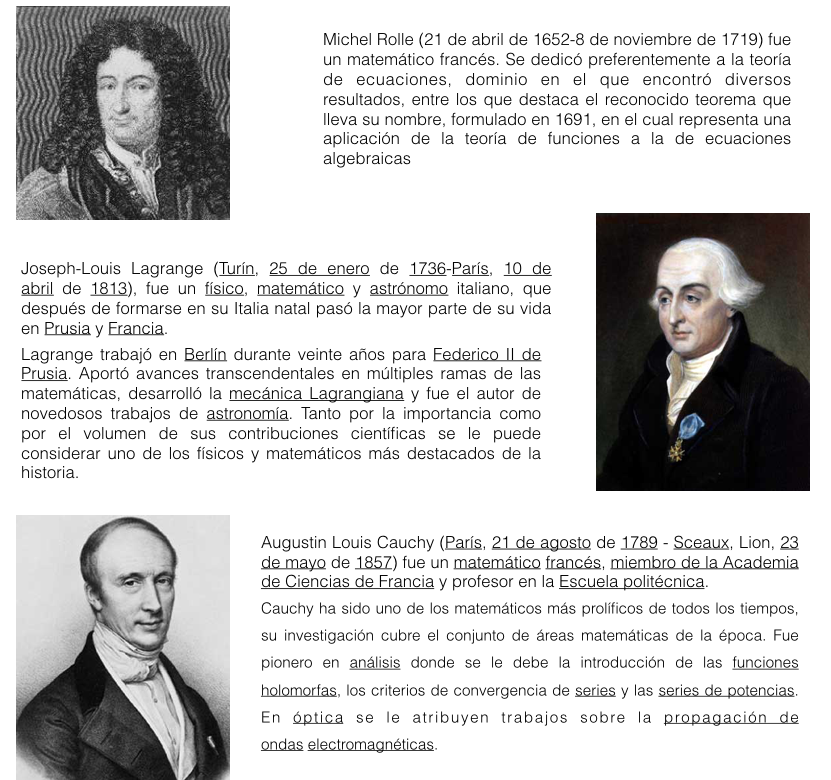
\includegraphics[width=1\textwidth]{imagenes/imagenes05/T05IM44.png}
		\end{figure}
		
		\begin{figure}[]
			\centering
			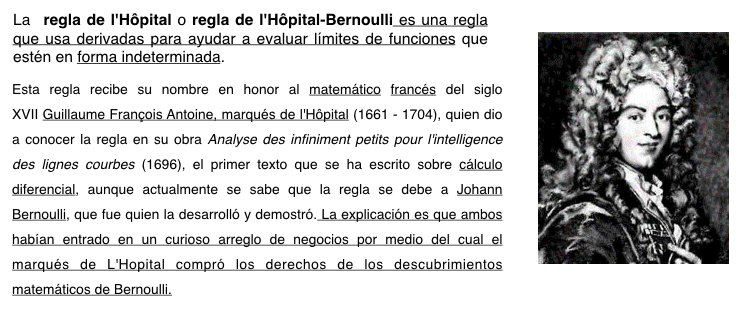
\includegraphics[width=1\textwidth]{imagenes/imagenes05/T05IM45.png}
		\end{figure}
		
		\subsection{Infinitésimos equivalentes}
		
		\begin{equation*}
		\alpha \sim \beta \leftrightarrow \underset {x\to a}{lim}\; {\dfrac {\alpha}{\beta}} = 1
		\end{equation*}
		
	
		 \begin{teor}{PRINCIPIO DE SUSTITUCIÓN}: Si en el cálculo de un límite se sustituye un factor o divisor por un infinitésimo equivalente, el límite no varía. (!`No se debe realizar sustitución si está sumando o restando!)
		 
		
		 \end{teor} Sustitución de infinitésimos equivalentes.
		 
	
		 
		 \begin{proof}
		 Supongamos $x\to a: \; \alpha (x) \sim \beta (x) \Rightarrow \underset {x\to a}{lim }\; { \dfrac {\alpha (x)}{ f(x) } }= \underset {x\to a}{lim }\;  
		 {\left(  \dfrac {\alpha (x)}{ f(x) } \cdot \dfrac {\beta (x)}{ \beta (x) } \right)}=  
		 \cancelto{1}{\underset {x\to a}{lim }\; { \dfrac {\alpha (x)}{ \beta (x) } } }
		 \cdot \underset {x\to a}{lim }\; { \dfrac {\beta (x)}{ f(x) } } =\underset {x\to a}{lim }\; { \dfrac {\beta (x)} {f(x)}}$ El límite es el mismo si sustituimos $\alpha (x)$ por su infinitésimo equivalente $\beta (x)$.
		 \end{proof}
		 

		\underline{Son infinitésimos equivalentes, cuando $x\to 0$}:
		 
		
		$\boxed{ \; \sin x \sim x\:; \quad \cos x \sim 1 - \frac 1 2 x^2\:; \quad \tan x \sim x\:; \quad e^x	 \sim 1 + x\:; \quad \ln (1+x) \sim x \; }$ 



	
\section{Ejercicios de Teoremas relativos a funciones derivables} 

\subsection{Ejercicios de resueltos de Teoremas relativos a funciones derivables}

	\begin{ejre} Comprueba que $f(x)=x^3-18x$ verifica las hipótesis del T. de Rolle en el intervalo $[0,3\sqrt{2}]$ y encontrar el punto que asegura el teorema
		
	\end{ejre}
	\begin{proofw}\renewcommand{\qedsymbol}{$\diamond$}	
		
		Al ser $f$ una función polinómica, es ctna. y dvble. en todo $\mathbb R$. Falta comprobar la tercera hipótesis: $f(0)=0$; $f(3\sqrt{2})=(3\sqrt{2})^3-18(3\sqrt{2})=54\sqrt{2}-54\sqrt{2}=0$, efectivamente $f(0)=f(3\sqrt{2})$
	\end{proofw}
	
	
	
	
	\begin{ejre} Comprobar si $f(x)=|x-2|$ cumple las hipótesis del Th. de Rolle en $[0,4]$
		
	\end{ejre}
	
	\begin{proofw}\renewcommand{\qedsymbol}{$\diamond$}	
	
	$f(x)=|x-2|=\begin{cases}
	2-x &; \;  0\le x<2 \\
	x-2 &; \;   2 \le x \le 4
	\end{cases} \quad \to \quad f'(x)=\begin{cases}
	-1 &; \;   0<x<2 \\
	1 &; \;   2<x<4 
	\end{cases}$
	
	$\nexists f'(2): \; f'_-(2)=-1\neq 1 =f'_+(2))$
	
	Aunque, evidentemente f es ctna en todo $\mathbb R$ y $f(0)=f(4)=2$, no se cumple la segunda hipótesis de que $f$ sea dvble.en $]0,4[$, ya que $\nexists f'(2)$ con $2\; \in \; ]0,4[$. Luego no se puede aplicar el teorema.
	\end{proofw}
	
	
	\begin{ejre} Aplica el Th. del Valor Medio en $[-1,3]$ a la función $f(x)=x^3$
		
	\end{ejre}
	\begin{proofw}\renewcommand{\qedsymbol}{$\diamond$}	
	
	Al ser $f$ polinómica es ctna y dvble en todo $\mathbb R$, en particular, será ctna. en $[-1,2]$ y dvble. en $]-1,3[$. Al cumplirse las hipótesis del Th. de V. M., aplicamos el mismo y la tesis nos asegura que $\exists \; c\;\in\ ]-1,3[ \quad / \quad f'(c)=\dfrac {f(3)-f(-1)}{3-(-1}$
	
	$f'(c)=3c^2=\dfrac {27-(-1)}{3-(-1}=\dfrac {28}{4}= 7 \to c^2= \dfrac 7 3 \to c= \pm \sqrt{\dfrac 7 3} \approx \pm 1.53$
	
	Como $ c\;\in\ ]-1,3[ \to c=+\sqrt{\dfrac 7 3}$

		
	\end{proofw}
	
	
	\begin{ejre} Para la función $f(x)=3x^2$, encontrar un punto en que la tangente a la curva en. dicho punto sea paralela a la cuerda que une los puntos $(0,0)$ y $(4,48)$.
		
	\end{ejre}
	\begin{proofw}\renewcommand{\qedsymbol}{$\diamond$}	
	
	Realmente, lo que nos piden en la aplicación geométrica del T.V.M. en el intervalo $[0,4]$.
	
	$f$, polinómica, es ctna. y dvble. en todo $\mathbb R$, por lo que lo es en el intervalo considerado. Al cumplirse las hipótesis del th., lo aplicamos:
	
	$\exists \; c\; \in \; ]0,4[ \; / \; f'(c)=\dfrac {f(4)-f(0)}{4-0}=m_{cuerda}$
	
	$f'(c)=6c=\dfrac {48-0}{4-0}=\dfrac {48}{4}= 12 \to c=2\; \in \; ]0,4[$
	
	\textcolor{gris}{Compruebe, si lo desea, el lector que la recta tangente a $f(x)$ en $x=2$ es paralela a la cuerda que pasa por $(0,f(0))$ y $(4,f(4))$.}
		
	\end{proofw}
	
	
	\begin{ejre} Aplicar, si es posible, el T.V.M. en el intervalo $[-2,0]$ a la función $y=f(x)=\begin{cases}
		\; \; \; \; \dfrac 1 x \; & \; -2\le x \le -1\\
		\dfrac {x^2-3}{2} \; & \; -1 < x \le 0
		\end{cases}	$
		
	\end{ejre}
	\begin{proofw}\renewcommand{\qedsymbol}{$\diamond$}	
		
		El T.V-M tiene solo dos hipótesis, que $f$ sea ctna en $[-2,0]$ y dvble en $]-2,0[$. Al ser ambos trozos continuos y dvbles $(x\neq 0; -2\le x\le-1)$, bastará solo con comprobar que $f$ en ctna. en $-1$ y dvble. en $-1$.
		
		$y=f(x)=\begin{cases}
		\; \; \; \; \dfrac 1 x \; & \; -2\le x \le -1\\
		\dfrac {x^2-3}{2} \; & \; -1 < x \le 0
		\end{cases}; \quad y'=f'(x)=\begin{cases}
		 -\dfrac 1 {x^2} \; & \; -2< x < -1\\
		\; \; \; x \; & \; -1 < x < 0
		\end{cases}	$	
		
		$f_-(-1)=-1=f_+(-1)$; $f$ ctna. en $x=-1$
		
		$f'_-(-1)=-1=f'_+(-1)$; $f$ dvble. en $x=-1$
		
		Luego $f(x)$ en ctna. en $[-2,0]$ y dvble. en $]-2,0[$, por el TVM $\exists \; c\; in\; ]-2,0[ \; / \; $
		
		$f'(c)=\dfrac {f(0)-f(-2)}{0-(-2)}= \dfrac {-3/2 - (-1/2)}{0-(-2)}= \dfrac {-1}{2}$
		
		Busquemos ese $c$ cuya existencia asegura el T.V.M.:
		
		$\circ\; \; $ si $-2<x<-1: \quad f'(c)=-\dfrac{1}{c^2}=-\dfrac 1 2 \to c^2=2 \to c=\pm\sqrt{2} \; $. En el intervalo considerado solo es válida la solución $c=-\sqrt{2} \; in \; ]-2,-1[$
		
		$\circ\; \; $ si $-1<x<0: \quad f'(c)=x=-\dfrac 1 2\; $ Solución también válida por estar en el intervalo considerado $c=-\dfrac 1 2 \; \in \; ]-1,0[$
		
		El problema tiene admite dos soluciones (El T.V.M. asegura que existe, al menos , una): $c=-\sqrt{2} \; \wedge \; c=-\dfrac 1 2$
		
	\end{proofw}


	\begin{ejre} Calcula $a$, $b$ y $c$ para que la función $f(x)= \begin{cases}
		x^2+ax+b \; ;&  x<2 \\
		cx+1 \; ;& x\ge2
		\end{cases}$ Cumpla las hipótesis de Th. Rolle en $[0,4]$ y aplíquese, si es posible.
		
	\end{ejre}
	\begin{proofw}\renewcommand{\qedsymbol}{$\diamond$}	
		
		Puesto que tenemos una función a trozos, ambos polinómicos, $f$ es ctna. y dvble en todo $\mathbb R$ excepto, tal vez, en el nexo $x=2$ donde estudiaremos la ctndad. y dvbdad.
		
		H1-Th Rolle: $f_-(2)=4+2a+b=2c+1=f_+(2) \to 2a+b+2c=-3$ (*ec.1) y la función será ctna. en $x=2$ y, por lo dicho anteriormente, ctna. en $[0,4]$
		
		H2-Th. Rolle $f'(x)= \begin{cases}
		2x+a \; ;&  x<2 \\
		c \; ;& x>2
		\end{cases} \quad \to \quad f'_-(2)=4+a=c$ (*ec.2) y la función será derivable en $x=2$ y, por lo dicho anteriormente, dvble.. en $]0,4[$
		
		H3-Th. Rolle: $f(0)=b; \; f(4)=4c+1 \to b=4c+1$ (*ec.3) y se cumplirá la tercera hipótesis del Th. de Rolle.
		
		Tenemos 3 ecuaciones con 3 incógnitas: $\begin{cases}
			2a+b+2c=-3 \\
			4+a=c \\
			b=4c+1
			\end{cases} \Rightarrow \small{a=-3; \wedge \; b=5; \; c=1}$
			
		En este caso: $f'(x)= \begin{cases}
		2x-3 \; ;&  x<2 \\
		1 \; ;& x>2
		\end{cases}$ 
		
		El th. de Rolle asegura que existe un $\lambda \; in \; ]0,4[\; ; / \; f'(\lambda)=0$
		
		$\circ \;$ si $0<x<2:\; f'(\lambda)=2\lambda-3=0 \to \lambda=3/2 \; \in ]0,2[$, solución válida.
		
		$\circ \;$ si $2 < x < 4 : \; f(\lambda)=1 \neq 0 \to \nexists \; \lambda=$, no hay solución en este subintervalo.
		
		$\circ \;$ si $x=-2:\; f'(-2)=1\neq 0$ Tampoco habría solución.
		
		La solución, única en este caso, es que el punto de derivada nula se da en $\lambda=3/2$		
		
	\end{proofw}
	
	\begin{ejre} Calcula los siguientes límites:
	\begin{multicols}{2}
	\begin{enumerate} [a) ]
	\item $\underset {x \to 0 }{lim} \; {\dfrac {e^x-1} {x} }$
	\item $\underset {x\to 1 }{lim}\; {\dfrac {1+\cos (\pi x)}{x^2-2x+1} }$
	\item $\underset {x\to 0^+ }{lim} \; { \dfrac {\mathrm{ln} (\cos (3x)} {\mathrm{ln}  (\cos (2x)} } $
	\item $\underset {x\to 0} {lim} \; {\dfrac {x-\sin x}{x^3}}$
	\item $\underset {x\to 0} {lim}\; { (1+2x) ^ {\left( \dfrac {1} {3x} \right) }} $
	\item $\underset {x\to 0}{lim}\; {x^{\; \sin x}}$
	\item $\underset {x\to 0 }{lim}\; {\left(\dfrac 1 x -\cosec x  \right)}$
	\item $\underset {x\to 0^+}{lim}\; {x^3 \; \mathrm{ln}x}$
	\item $\underset {x\to \infty}{lim}\;{ \left(  \dfrac {2^x+3^x}{2}   \right)  ^ { \dfrac {1}{x}  }   }$
	\item $\underset {x \to -3}{lim}\;{\dfrac {x^3-3x^2-45x-81}{x^3+3x^2-9x-27}}$
	\end{enumerate}
	\end{multicols}
		
	\end{ejre}
	\begin{proofw}\renewcommand{\qedsymbol}{$\diamond$}	Soluciones:
	
	$a) \quad \underset {x \to 0 }{lim} \; {\dfrac {e^x-1} {x} } =[0/0; \; ind:\; L'H]=\underset {x \to 0 }{lim} \; {\dfrac {e^x} {1} }=\dfrac 1 1 = 1$	
	
	$b) \quad \underset {x\to 1 }{lim}\; {\dfrac {1+\cos (\pi x)}{x^2-2x+1} } = [0/0; \; ind:\; L'H] = \underset {x\to 1 }{lim}\; {\dfrac {-\pi\; \sin (\pi x)}{2x-2} }= [0/0; \; ind:\; L'H] =\underset {x\to 1 }{lim}\; {\dfrac {-{\pi}^2\; \cos (\pi x)}{2} }= {\pi}^2/2$
	
	$c) \quad \underset {x\to 0^+ }{lim} \; { \dfrac {\mathrm{ln} (\cos (3x)} {\mathrm{ln}  (\cos (2x)} } = [0/0; \; ind:\; L'H] = \underset {x \to 0^+ } {lim} \; { \dfrac {\dfrac {-3\sin (3x)} {\cos (3x)} } { \dfrac {-2\sin (2x)}  {\cos (2x)} } }  = \dfrac 3 2 \; \underset {x\to 0^+}{lim}\;{\dfrac {\tan 3x}{\tan 2x}} = [0/0; \; ind:\; L'H] = \dfrac 3 2 \; \underset {x\to 0^+}{lim}\;{\dfrac {3(1+3\tan^2 3x)}{2(1+2\tan^2 2x)}}=\dfrac 9 4$
	
	$d) \quad \underset {x\to 0} {lim} \; {\dfrac {x-\sin x}{x^3}}=[0/0; \; ind:\; L'H] =\underset {x\to 0} {lim} \; {\dfrac {1-\cos x}{3x^2}}=[0/0; \; ind:\; L'H] = \underset {x\to 0} {lim} \; {\dfrac {\sin x}{6x}}=[0/0; \; ind:\; L'H] = \underset {x\to 0} {lim} \; {\dfrac {\cos x}{6}}= \dfrac 1 6$
	
	$e) \quad \underset {x\to 0} {lim}\; { (1+2x) ^ {\left( \dfrac {1} {3x} \right) }} = L =[1^\infty ; \; ind: \; \mbox{ tomamos logaritmos} ]$
	
	$\mathrm{ln} \;  L=  \underset {x\to 0} {lim}\;   \mathrm{ln} \;  {(1+2x)} ^ { \left( \dfrac {1} {3x} \right) } =[\mbox { aplicamos propiedades de los logaritmos} ] =$
	
	$= \underset {x\to 0}{lim} \;{ \dfrac {\mathrm{ln} (1+2x)}{3x} } = [0/0; \; ind: \; L'H]= \underset {x\to 0}{lim} \;{ \dfrac {\dfrac {2}{1+2x}}{3} }= \underset {x \to 0}{lim} \; {\dfrac {2}{3(1+2x)}}=2/3$
	
	Como $\mathrm{ln} \;L=3/2\to L=e^{3/2}$
	
	--- Al tratarse de la indeterminación $1^\infty$, también podríamos haber usado el método rápido del número $e$, visto en la sección \ref{sec-metodo-e}:
	
	$\underset {x\to 0} {lim}\; { (1+2x) ^ {\left( \dfrac {1} {3x} \right) }}  =[1^\infty:\; \mbox{ [método del número e] }= exp \left\{ \underset {x\to 0}{lim}\; { (1+2x-1) \cdot \dfrac {1}{3x} }  \right\} = exp \left\{ \underset {x\to 0}{lim}\; {\dfrac {2x}{3x}} \right\} =e^{2/3}$
	
	$f) \quad \underset {x\to 0}{lim} \; {{x} ^{\; \sin x}}=L= [0^0; \; ind: \; \mbox{ tomamos } \mathrm{ln}] \to \mathrm{ln}\; L= \underset {x\to 0}{lim } \; {\sin x \cdot \mathrm{ln} x} = [0\cdot \infty: \; \mbox{ convertimos el producto en un cociente }]=\underset{x\to 0}{lim}\;{\dfrac {\mathrm{ln}x}{\dfrac 1 x }}=[\infty / \infty: \; L'H]=\underset {x \to 0} {lim} \; { \dfrac { \dfrac {1}{x}}{- \dfrac {1}{x^2}} } =\underset {x\to 0}{lim}\;{(-x)}=0 \to \mathrm{ln}L=0 \to L=e^0=1$
	
	$g) \quad \underset {x\to 0 }{lim}\; {\left(\dfrac 1 x -\cosec x  \right)}= \underset {x\to 0 }{lim}\; {\left(\dfrac 1 x - \dfrac 1 {\sin x}  \right)}=[\infty - \infty: \mbox{ convirtamos la resta} $
	$ \mbox{ en un cociente ]}= \underset {x\to 0}{lim}\;{\dfrac {\sin x - x}{x \; sinx}}=[0/0:\; L'H] = 
	\underset {x\to 0}{lim}\;{\dfrac {\cos x - 1}{\sin x + x \cos x}}=[0/0:\; L'H]= \underset {x\to 0}{lim}\;{\dfrac {-\sin x }{\cos x + (\sin x + x (-\sin x)) }}= 0/1=0$
	
	$h) \quad \underset {x\to 0^+}{lim}\; {x^3 \; \mathrm{ln}x}=[0 \cdot \infty: \mbox { convirtamos en cociente }]=\underset {x\to 0^+}{lim}\;{\dfrac{\mathrm{ln}x}{x^3}}=\underset {x\to 0^+}{lim}\; {\dfrac {- \dfrac 1 x }{3x^2}}=\underset {x\to 0^+}{lim}\;{\dfrac {-1}{3x^3}}=-\infty$.
	
	$i) \quad \underset {x\to \infty}{lim}\;{ \left(  \dfrac {2^x+3^x}{2}   \right)  ^ { \dfrac {1}{x}  }   } = [\infty ^0: \; ind: \mbox { tomamos logaritmos }]=L $
	
	$\mathrm{ln} \; L = \underset {x\to \infty}{lim}\;{\dfrac {\dfrac {2^x+3^2}{2}}{x}}= \underset {x\to \infty}{lim}\;{\dfrac {2^x+3^x}{2x}} [\infty / \infty: \; l'H \;$ (bastaría recordar que $a^x>>x$ para $x>>1$ y $a>1$ - órden de infinitos]$=\underset{x\to \infty}{lim}\;{\dfrac {2^x\; \mathrm{ln}2+3^x\; \mathrm{ln}3}{2}}=\dfrac {\infty}{2}=\infty \quad \Rightarrow \quad \mathrm{ln}\; L=\infty \to L=e^{\infty}=\infty$.
	

	$j) \quad \underset {x \to -3}{lim}\;{\dfrac {x^3-3x^2-45x-81}{x^3+3x^2-9x-27}} = [0/0; \; ind: \mbox{ Ruffini o l'H }] \underset {x \to -3}{lim}\;{\dfrac {3x^2-6x-45}{3x^2+6x-9}}=[0/0; \; ind: \mbox{ Ruffini o l'H }]=\underset {x \to -3}{lim}\;{\dfrac {6x-6}{6x+6}}=\dfrac {-24}{-12}=2$
	\end{proofw}
	
	
	
	\begin{ejre} $\divideontimes$ Utilizando infinitésimos equivalentes, calcula los siguientes límites:
	
	$\sin x \sim x\:; \quad \cos x \sim 1 - \frac 1 2 x^2\:; \quad \tan x \sim x\:; \quad e^x	 \sim 1 + x\:; \quad \ln (1+x) \sim x$ 
	
		\begin{multicols}{2}
		
	\begin{enumerate} [a) ]
	\item $\underset {x \to 0 }{lim} \; {\dfrac {e^x-1} {x} }$
	\item $\underset {x\to 0 }{lim}\;{\dfrac {\tan x}{x}}$
	\item $\underset {x\to 0}{lim}\;{\dfrac {1-cos x}{x}}$
	\item $\underset {x\to 0 }{lim}\;{\dfrac {x-\sin 3x}{\sin 5x}}$
	\item $\underset {x\to a}{lim}\;{ \dfrac {\sin x - \sin a}{x-a} }$
	
	\end{enumerate}
	\end{multicols}
	\end{ejre}
	
	
	
	\begin{proofw}\renewcommand{\qedsymbol}{$\diamond$}	
	Soluciones:
	
	$a)\quad \underset {x \to 0 }{lim} \; {\dfrac {e^x-1} {x} }=[e^x \sim 1+x]=\underset {x \to 0 }{lim} \; {\dfrac {1+x-1} {x} }=1$
	
	$b) \quad \underset {x\to 0 }{lim}\;{\dfrac {\tan x}{x}}=[\tan x \sim x]=\underset {x\to 0 }{lim}\;{\dfrac { x}{x}}=1$
	
	$c) \quad \underset {x\to 0}{lim}\;{\dfrac {1-cos x}{x}}=[\cos x \sim 1-\frac 1 2 x^2]=\underset {x\to 0}{lim}\;{\dfrac {1-(1-\frac 1 2 x^2)}{x}}=\underset {x\to 0}{lim}\;{\dfrac {\frac 1 2 x^2}{x}}=\underset {x\to 0}{lim}\;{\frac 1 2 x}=0$
	
	$d) \quad \underset {x\to 0 }{lim}\;{\dfrac {x-\sin 3x}{\sin 5x}} =[\mbox{ rompemos la fracción en dos }] = \left( \underset {x\to 0 }{lim}\;{ \dfrac {x}{\sin 5x} } \right) - \left( \underset {x\to 0 }{lim}\;{ \dfrac {\sin 3x}{\sin 5x} } \right) =[\sin ax 	\sim ax]= \left( \underset {x\to 0 }{lim}\;{ \dfrac {x}{ 5x} } \right) - \left( \underset {x\to 0 }{lim}\;{ \dfrac {3x}{ 5x} } \right) = \frac 1 5 -\frac 3 5=-\frac 2 5$
	
	$e) \quad \underset {x\to a}{lim}\;{ \dfrac {\sin x - \sin a}{x-a} }=\left[ \mbox { fórmula: }  \sin x - \sin a = 2 \;  \sin {\left( \dfrac {x-a}{2} \right)}   \cdot \cos { \left( \dfrac {x+a}{2} \right) } \; \right] =$
	
	$= \underset {x\to a}{lim}\;{ \dfrac {2 \;  \sin {\left( \dfrac {x-a}{2} \right)}   \cdot \cos { \left( \dfrac {x+a}{2} \right) }}{x-a} } =$
	
	$= \underset {x\to a}{lim}\;{ \dfrac {2 \;  \sin {\left( \dfrac {x-a}{2} \right)}   \cdot }{x-a} } \cdot \underset {x\to a}{lim}\;{ \cos { \left( \dfrac {x+a}{2} \right) } } =$
	
	$=\left[ \sin \left ( \dfrac {x-a}{2}\right) \sim \dfrac {x+a}{2} \right] = \underset {x\to a}{lim}\;{ 2 \; \dfrac { (x-a) }{\dfrac {x-a}{2}} } \cdot \underset {x\to a}{lim}\;{ \cos { \left( \dfrac {x+a}{2} \right) } }= 2 \; \frac 1 2 \; cos(a) = \cos a$ 
	\end{proofw}
	

	





	\begin{ejre} Calcula $\underset{x\to 0}{lim}\;{\dfrac {\sin x}{x}}$ (Ver ejercicio resuelto \ref{ejem:sinx/x})
	\end{ejre}
	
	\begin{proofw}\renewcommand{\qedsymbol}{$\diamond$}	
		
		Resolveremos el problema de dos maneras (más) distintas:
		
		R DE L'Hôpital: $\underset{x\to 0}{lim}\;{\dfrac {\sin x}{x}}=[0/0; \; ind: \;  L'H] =\underset{x\to 0}{lim}\;{\dfrac {\cos x}{1}}= \dfrac {\cos 0}{1}=\dfrac 1 1 = 1$
		
		INFINITES. EQUIV.: $ \underset{x\to 0}{lim}\;{\dfrac {\sin x}{x}}= [\; x\to 0: \; \sin x \sim x \; ]=\underset{x\to 0}{lim}\;{\dfrac { x}{x}}= \underset{x\to 0}{lim}\;{1}=1$
	\end{proofw}




 \subsection {Ejercicios propuestos de Teoremas relativos a funciones derivables}

\begin{enumerate} 
\item Psra $y=x^3-5x^2+3x+2$, aplica si es posible, el T.V.M. en $[0,4]$


\rightline{\textcolor{gris}{Solución: Hay dos puntos $c=\dfrac {5 \pm  \sqrt{13}}{3}$ }}

\item La función $f(x)=|\cos x|$ toma el mismo valor en los extremos del intervalo $[0,\pi]$. ?`existe algún punto, en el interior de este intervalo, donde la derivada sea nula?

\rightline{\textcolor{gris}{Solución: $\nexists \; f'(0)$, no se cumplen las hip. del Th. Rolle, no se puede asegurar la hipótesis. }}


\item Sea $f(x)$ una función continua y derivable tal que $f(0)=3$. Calcula el valor de $f(5)$ para asegurar que en $[0,5]$ existe un punto $c$ con derivada nula ($f'(c)=0$).
 
\rightline{\textcolor{gris}{Solución: Th. Rolle: $f(5)=43$ }}


\item Calcula $a$ y $b$ para que en $[2,6]$ se cumplan las hip. del T.V.M. y, aplíquese en su caso, para la función $f(x)=\begin{cases}
	ax-3 ; \; & 2\le x < 4 \\
	-x^2+10x+b ; \; & 4\le x \le 6
	\end{cases}$

\rightline{\textcolor{gris}{Solución: $a=2 ; \; b=19; \; \quad   c=9/2$ }}


\item Calcula los límites de las siguientes funciones:
\begin{multicols}{2}
\begin{enumerate}[a) ]
\item $\underset {x\to 0}{lim}\;{\dfrac {\mathrm{ln}x}{x}}$
\item $\underset {x\to o}{lim}\;{\dfrac {\sin x - x}{\tan x - x}}$
\item $\underset {x\to 0 }{lim}\;{\dfrac {(1-\cos x)\; \sin x}{x^2}}$
\item $\underset {x\to 0 }{lim}\;{\dfrac {x-\sin x}{\tan x - \sin x}}$
\item $\underset {x\to 0 }{lim}\;{\dfrac 1 {\sin x}- \dfrac 1 x}$
\item $\underset {x\to 0 }{lim}\;{x^x}$
\item $\underset {x\to 0}{lim}\;{ (1-\cos x){2x}}$
\item $\underset {x\to \infty }{lim}\;{(\mathrm{ln}x)^ {\dfrac {1}{e^x}}}$
\item $\underset {x\to 1}{lim}\;{\dfrac{x}{\mathrm{ln}x} - \dfrac {1}{\sin(x-1)}}$
\item $\underset {x\to \infty}{lim}\;{x\left(2^{\dfrac 1 x}-1 \right)}$
\item $\underset {x\to 1}{lim}\;{x^{\dfrac {1}{1-x}}}$
\end{enumerate}	
\end{multicols}



\rightline{\textcolor{gris}{Solución: $a)\; 0\quad b)\; -1/2 \quad c); 0 \quad d)\; 1/3 \quad e); 0\quad f)\; 1\quad g)\; 1\quad h)\; 1\quad i)\; 3/2 \quad j) \; \mathrm{ln}2 \quad k)\; 1/e$ }}
	
\end{enumerate}

	
	
\section{Representación gráfica de funciones explícitas}

Una de las importantes aplicaciones de lo aprendido hasta ahora es la `representación gráfica de funciones'. Para ello, aunque el método es, muchas veces redundante, se basa en los siguientes pasos:

	\begin{enumerate}
	\item DOMINIO Y CONTINUIDAD: valores para los que f(x) está definida y si presenta algún tipo de discontinuidad en su dominio de definición.
	\item SIMETRÍAS Y PERIODICIDAD: Recordad que si $f(-x)=f(x)$, la función es PAR y simétrica respecto del eje $OY$. Si  $f(-x)=-f(x)$. la función es IMPAR y simétrica respecto del origen de coordenadas.

	Una función era periódica de periodo $T$ si $f(x+T)=f(x)$. Bastaría con estudiar $f(x)$ en un periodo y repetirla.

	\item  CORTES CON LOS EJES:	 $x=0 \to y?; \quad y=0 \to x?$
	
	Recordad que una función puede cortar al eje $OY$ una o ninguna vez, para los cortes con el eje $OX$ no hay ninguna restricción.
	
	\item ASÍNTOTAS: Recordad lo visto en la subsección \ref{subsec-asintotas}
	
		\hspace{10mm} $\circ\;$ Asíntota Vertical (AV): Decimos que $x=x_0$ es AV de $f(x)$ si $\underset{x\to x_0}{lim}\;{f(x)}=\infty$. Suelen ser valores que anulan el denominador de la función.
		
		Independientemente de que existan o no AV, llamamos:
		
		\hspace{10mm} $\circ\;$ Asíntota Horizontal (AH): Decimos que la recta horizontal $y=b\in \mathbb R$ es AH de $f(x)$ si $\underset{x\to \infty}{lim}\;{f(x)}=b$
		
		En el caso de que no existan AH, puede que la función en el infinito se comporte según una recta oblícua, $y=mx-n$, donde $m$ y $n$ se calculan como se indica a continuación:
		
		\hspace{10mm} $\circ\;$ Asíntota Oblícua (AO), si no hay AH: Decimos que la recta $y=mx+n$ es AO de $f(x)$ si $\underset{x\to x_0}{lim}\;{\dfrac {f(x)} {x} }=m\in \mathbb R$ y $\underset{x\to x_0}{lim}\;{(f(x)-mx)}=n \in \mathbb R$
		
	\item INF. PRIMERA DERIVADA: Los $PC(y')$ se representan en $\mathbb R$ y donde:
	
	 $y'>0 \to y \; \nearrow; \quad y'<0 \to y \; \searrow \;$.  Si hay cambio en el crecimiento a la dcha. e izqda. de un punto $a$ y $\exists \; f(a)$, decimos que en $x=a$ hay un extremos relativo. (También se puede usar el criterio de la derivada segunda - teorema \ref{teor-crit-deriv2})
	 
	 \item INF. SEGUNDA DERIVADA: Los $PC(y'')$ se representan en $\mathbb R$ y donde:
	
	 $y''>0 \to y \; \cup; \quad y'<0 \to y \; \cap \;$.  Si hay cambio en la curvatura a la dcha. e izqda. de un punto $a$ y $\exists \; f(a)$, decimos que en $x=a$ hay un punto de inflexión. 
	 
	 \item Con toda la información recogida en los puntos anteriores, inténtese representar la función.	 

	
\end{enumerate}




	
\section{Ejercicios de representación de funciones}




\subsection{Ejercicios resueltos de representación de funciones}


\begin{ejre} Representa la función $y=x^3-3x^2+4$
	
\end{ejre}

\begin{proofw}\renewcommand{\qedsymbol}{$\diamond$}	

$f$ ctna, dvble, en todo su dominio $\mathbb R$ y carece de asíntotas por ser un polinomio.


Cortes: $x=0 \to y=4; \quad y=0=x^3-3x^2+4 = [\mbox{ Ruffini }]=(x+1)(x-2)^2 \to x=-1 \; \wedge \; x=2 \quad \Rightarrow \quad \textbf {(0,4); \; (-1,0); \; (2,0)}$

\begin{multicols}{2}
Monotonía y extremos: $y'=3x^2-6x \to PC(y')\to y'=0=3x(x-2) \to x=0 \; \wedge \; x=2$ Al ser $y'$ una parábola hacia arriba que corta a $OX$ en $x=0 \; \wedge \; x=2$, tendremos:  $x<0: \;y'> to y\; \nearrow; \quad 0<x<2: \; y'<0 \to y\; \searrow \quad x>2; \; y'>0 \to y\; \nearrow$ Habrá un { $\textbf{M(0,4)}$} y un $\textbf{m(2,0)}$.

Curvatura e inflexiones: $y''=6x-6  \to PC(y'') \to y''=0=6x-6 \to x=1$. Analizando el signo de $y''$ tenemos: $x<1:	\; y''<0 \to y\; \cap \; ; \quad x>1:\; y''>0 \to y\; \cup$. Hay pues una $I(1,f(1))= \textbf{I(1,2)}$

Con todo ello (fijarse en lo destacado en negrita), intentamos un esbozo de la gráfica.
	
		\begin{figure}[H]
			\centering
			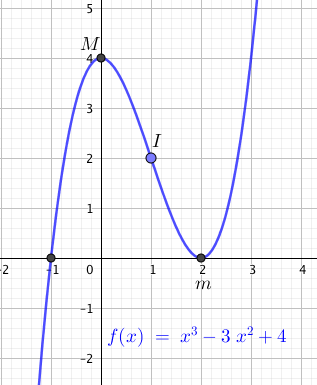
\includegraphics[width=0.3\textwidth]{imagenes/imagenes05/T05IM30.png}
		\end{figure}
\end{multicols}
	
\end{proofw}


\begin{ejre} Representa la función: $y=\dfrac {1}{x^2+1}$
	
\end{ejre}

\begin{proofw}\renewcommand{\qedsymbol}{$\diamond$}	

$Dom(f)=\mathbb R: \quad x^2+1\neq 0$

Costes, solo $\textbf{(0,1)}$

AH: $\underset {x\to \infty}{lim }\;{ \dfrac {1}{x^2+1}  }=0 \to \textbf{y=0:\; AH}$

Crecimiento: $y'=-\dfrac {2x}{(1+x^2)^2} \to PC(y) \to y'=0 \to x=0$

$x<0: \; y'>0 \to y\; \nearrow; \quad x>0:\; y'<0 \to y\; \searrow$ Hay un $\textbf{M(0,0)}$
	
Curvatura: $y''=\dfrac {-2(x^2+1)^{\cancel{2}}-(-2x)2\cancel{(x^2+1)}(2x)}{(x^2+1)^{\cancel{4}3}}=\dfrac {6x^2-2}{(x^2+1)^3}$
\begin{multicols}{2}
	
$PC(y'') \to y''=0 \to x=\pm \sqrt{3}/3$ Como el denominador de $y''$ es siempre positivo, el signo de $y''$ lo da el numerador, que es una parábola hacia arriba con cortes en $OX$ en $\pm \sqrt{3}/3$, por lo que: $x<-\sqrt{3}/3:\; y''>0 \to y\; \cup \quad -\sqrt{3}/3<x<\sqrt{3}/3:\; y''<0 \to y\; \cap \quad x>\sqrt{3}/3: \; y''>0 \to y\; \cup$. Hay pues dos inflexiones en, aproximadamente,  $\textbf{I( -0.58, 0.75)}$ y $\textbf{I( 0.58, 0.75)}$

Dibujemos la función:
		\begin{figure}[H]
			\centering
			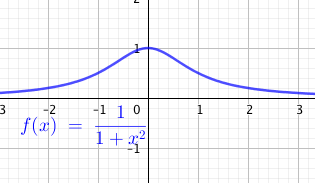
\includegraphics[width=0.4\textwidth]{imagenes/imagenes05/T05IM31.png}
			\caption{Curva de Agnesi.}
		\end{figure}
\end{multicols}

\end{proofw}


\begin{ejre} Representa la función: $y=\dfrac {x^2+1}{x^2-2x}$

	
\end{ejre}

\begin{proofw}\renewcommand{\qedsymbol}{$\diamond$}	
	$Dom(f)=\mathbb R \sim \{0,2\}$, ya que $x^2-2x=x(x-2)=0 \leftrightarrow x=0 \; \wedge \; x=2$
	
	Cortes: $x=0 \to \nexists \; y \; ; \quad y=0 \to x^2+1=0: \; \nexists x$. \textbf{La función no corta a los ejes coordenados}.
	
	Asíntotas:  como $\underset {x\to 0}{lim }\;{\dfrac {x^2+1}{x^2-2x}}=1/0=\infty \to \textbf{x=0: \; AV}\; ; \quad  \underset {x\to 2}{lim }\;{\dfrac {x^2+1}{x^2-2x}}=5/0=\infty \to \textbf{x=2: \; AV}$
	
		$\underset {x\to \infty}{lim}\; {\dfrac {x^2+1}{x^2-2x}}=1 \to \textbf{y=1: \; AH}$
		
		\noindent Crecimiento: $y'=\cdots=\dfrac {-2x^2-2x+2}{(x^2-2x)^2} \to \begin{cases}
 			\nexists \; y' \to x=0 \; \wedge \; x=2 \\
 			y'=0=-2x^2-2x+2 \to x=\dfrac {-1\pm \sqrt{5}}{2}
 			\end{cases}$
 			
 			Estudiemos el signo de $y'$ en una tabla:
 			
 	\begin{table}[H]
 	\centering
	\begin{tabular}{|c|c|c|c|c|c|}
	\hline
 	Crecto.& $]-\infty,\frac {-1-\sqrt{5}}{2}[$ & $]\frac {-1-\sqrt{5}}{2},0[$ & $]0,\frac {-1+\sqrt{5}}{2}[$ & $]\frac {-1+\sqrt{5}}{2},2[$  & $]2,\infty[$ \\ \hline
 	$y'$& $-$ &  $+$  & $+$   &  $-$  &  $-$  \\ \hline
 	$y$& $\searrow$ & $\nearrow$ &  $\nearrow$ & $\searrow$ & $\searrow$ \\ \hline
	\end{tabular}
	\end{table}
	
		Se observa un $\textbf{m(-1.62,0.62}$ y un $\textbf{M(0.62,-1.62}$
		
		Como la curvatura se va a complicar mucho, intentaremos el dibujo con lo estudiado hasta ahora.
		
		\begin{figure}[H]
			\centering
			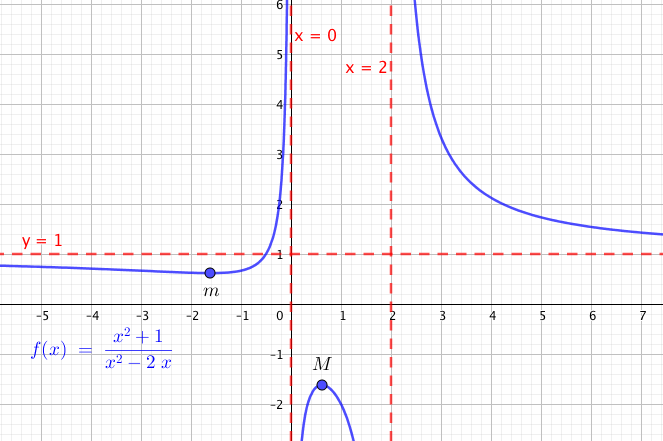
\includegraphics[width=0.9\textwidth]{imagenes/imagenes05/T05IM32.png}
		\end{figure}
		
\end{proofw}


\begin{ejre} Representa la función: $y=\dfrac {x^2-5x+7}{x-2}$
	
\end{ejre}

\begin{proofw}\renewcommand{\qedsymbol}{$\diamond$}	

Dominio: $D(f)=\mathbb R \sim \{2\}$

Cortes: $x=0 \to y=-7/2; \quad y=0 \to \nexists x$. Cortes en $\textbf { (0,-7/2) } $

Asíntotas: $\underset{x\to 2}{lim}\;{\dfrac {x^2-5x+7}{x-2}}=1/0=\infty \to \textbf{ x=2: \; AV   }  $

$\underset {x\to \infty}{lim}\;{\dfrac {x^2-5x+7}{x-2}}=\infty \to {\nexists \; AH} $. Busquemos si hay AO:

$m=\underset {x\to \infty}{lim}\;{\dfrac {f(x)}{x}}=\underset {x\to \infty}{lim}\;{ \dfrac {x^2-5x+7}{x(x-2)} }=1$

$n=\underset {x\to \infty}{lim}\; {(f(x)- 1\cdot x)}=
\underset {x\to \infty}{lim}\;{\left( \dfrac {x^2-5x+7}{x-2}-x \right)}=\cdots=\underset {x\to \infty}{lim}\;{\left( \dfrac {-3x+7}{x-2} \right)}=-3 \quad \to \quad \textbf{y=x-7: \; AO }$

Crecimiento: $y'=\cdots= \dfrac {x^2-4x+3}{(x-2)^2} \to \begin{cases}
 \nexists \; y' \to x=2 \\
 y'=0=x^2-4x+3 \to x=1; \; x=3	
 \end{cases}$
 
 Estudiamos el signo de $y'$ en una tabla (pensando un poco no es necesario: el denominador siempre es positivo y el numerador, que dictará el signo, es una parábola).
 
 	\begin{table}[H]
 	\centering
	\begin{tabular}{|c|c|c|c|c|}
	\hline
 	Crecto. & $]-\infty,1[$ & $]1,2[$ & $]2,3[$ & $]3,\infty[$ \\ \hline
 $y'$	& $+$ & $-$ & $+$ & $-$ \\ \hline
  $y$	& $\nearrow$ &$\searrow$  & $\searrow$ & $\nearrow$ \\ \hline
	\end{tabular}
	\end{table}
	
	Hay un $\textbf{M(1,-3)} $ y un $\textbf{m(3,1)}$
	
	Con la información recogida intentamos dibujar la función:
	
	\begin{figure}[H]
		\centering
		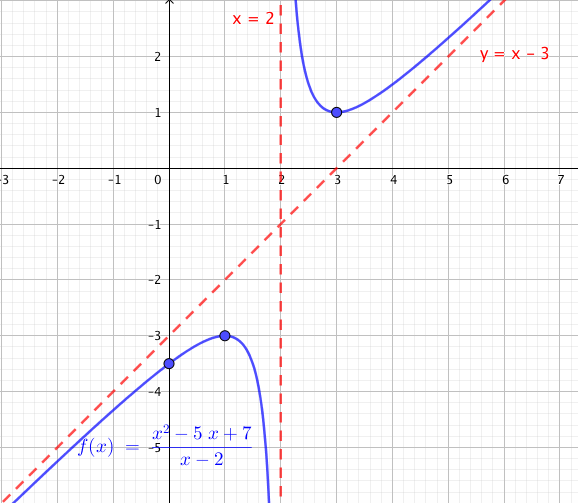
\includegraphics[width=0.9\textwidth]{imagenes/imagenes05/T05IM33.png}
	\end{figure}
	
\end{proofw}




\begin{ejre} Representa una función $y=f(x)$ sabiendo que $D(f)=\mathbb R \sim \{-2\}$. Es derivable en todo su dominio $\underset {x\to \pm\infty}{lim}\;{f(x)}=\mp 1\; \; $; $\; \underset {x\to 2}{lim}\; {f(x)}=\infty \; $ ; $\; f(0)=0; \; f/7)=0; $ ; $f'(x)=0 \leftrightarrow x=4 \; $ ; $\; f(4)=2\; ; \; f''(4)<0$ , tambien sabemos que $x<-2: \;  y'>0 \to y\; \nearrow$
	
\end{ejre}

\begin{proofw}\renewcommand{\qedsymbol}{$\diamond$}	

Al ser $f'(4)=0\; \wedge \; f''(4)<0 \; \wedge \; f(4)=2$, deducimos que hay un máximo en $M(4,2)$

También sabemos que $f$ será creciente en $x<-2$

Para que se cumplan todas las propiedades (verde), la función más sencilla la hemos dibujado en azul y hemos necesitado introducir dos inflexiónes (en verde) que no menciona el problema.

	\begin{figure}[H]
		\centering
		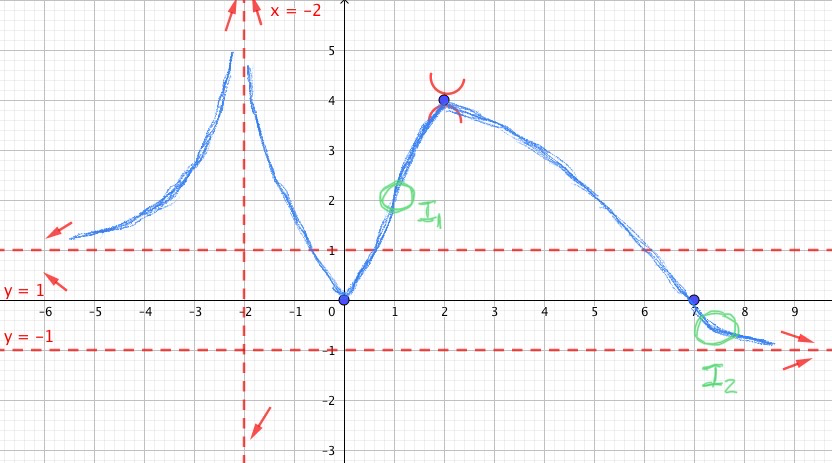
\includegraphics[width=0.85\textwidth]{imagenes/imagenes05/T05IM35.png}
	\end{figure}
	
\end{proofw}


\begin{ejre} Representa la función $y=|x|-|x-3|-|x+1|$
	
\end{ejre}

\begin{proofw}\renewcommand{\qedsymbol}{$\diamond$}	
  
  Primero romperemos la función a trozos:
\begin{multicols}{2}
	
Recordando lo aprendido el el ejercicio \ref{ejre:rompe-trozos}, sobre romper funciones a trozos, se deja al lector que compruebe que:
	

$y=\begin{cases}
-x-4 & \mbox { si }	x<-1 \\
x-2 & \mbox { si }	-1\le x < 0 \\
3x-2 & \mbox { si } 0\le x < 3 \\
x+4 & \mbox { si } x \ge 3
\end{cases}$

Como la función es tan básica no requiere de mayor estudio que dibujar sus cuatro trozos rectilíneos, aunque se sugiere al lector que busque los ceros y la monotonía y extremos.

\begin{figure}[H]
		\centering
		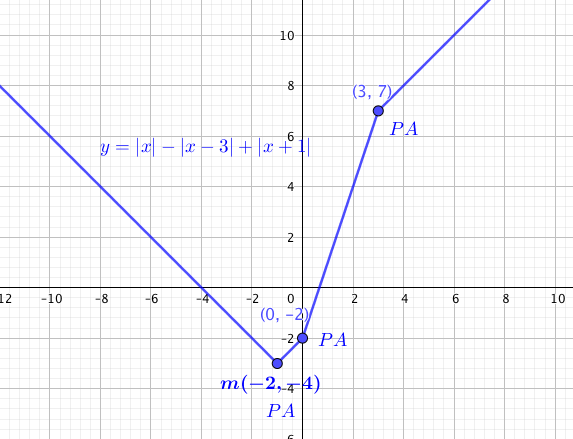
\includegraphics[width=0.5\textwidth]{imagenes/imagenes05/T05IM36.png}
	\end{figure}
\end{multicols}

\end{proofw}

\begin{ejre} Representa la función $y=\dfrac {\mathrm{ln}|x|}{x}$
	
\end{ejre}

\begin{proofw}\renewcommand{\qedsymbol}{$\diamond$}	

Obviamente, $y=f(x)=\begin{cases}
					\dfrac {\mathrm{ln}(-x)}{x} &; \; x<0 \\
					\dfrac {\mathrm{ln}(x)}{x} &; \; x>0 
					\end{cases}\; \; \;  \nexists \;  f(0)$
					
Dominio: $D(f)=\mathbb R \sim \{0\}$

Cortes: $x=0 \to \nexists \; y\; ; \quad y=0=\mathrm{ln}|x| \to |x|=1 \to x=\pm 1$. Los únicos puntos de corte son $\textbf{(-1,0)}$ y  $\textbf{(1,0)}$

Asíntotas: estudiemos que ocurre cerca del cero y en $\pm \infty$:

$\underset {x\to o^-}{lim}{\dfrac {\mathrm{ln}(-x)}{x}} = -\infty/o^-=+\infty \qquad \underset {x\to o^+}{lim}{\dfrac {\mathrm{ln}(x)}{x}} = -\infty/o^+=-\infty \quad $ 


!`$ \; x \to 0^- \rightarrow y\to +\infty \; ; \quad  x \to 0^+ \rightarrow y \to -\infty \; $ !

$\underset {x\to -\infty}{lim}{\dfrac {\mathrm{ln}(-x)}{x}} = [x=-t] = \underset {t\to +\infty}{lim}{\dfrac {\mathrm{ln}(t)}{-t}}= [\infty / \infty: 	\; L'H]=\underset {t\to +\infty}{lim}{\dfrac {\dfrac 1 t}{-1}} =\underset {t\to +\infty}{lim}{ -\dfrac 1 t }=0$

$\underset {x\to +\infty}{lim}{\dfrac {\mathrm{ln}(x)}{x}} = [\infty / \infty: 	\; L'H]= \underset {x\to +\infty}{lim}{ -\dfrac 1 x }=0 \qquad \textbf{y=0:\; AH}$

Monotonía:   $y'=f'(x)=\begin{cases}
					\dfrac{1-\mathrm{ln}(-x)}{x^2} &; \; x<0 \\
					\dfrac{1-\mathrm{ln}(x)}{x^2} &; \; x >0 
					\end{cases}\; \; \;  \nexists \;  f'(0)$
					
$PC(y')=\begin{cases}
\nexists \;  f'(x) \leftrightarrow x=0 \\
y'=0: \; \begin{cases}
 			x<0: \; ln(-x)=1 \to -x=e \leftarrow x=-e\\
 			x>0: \; ln(x)=1 \to x=e 
 			\end{cases}	
\end{cases}$

Estudiamos los signos de $y'$ en los intervalos en que los $PC$ dividen al eje $\mathbb R$.

	\begin{table}[H]
	\centering
	\begin{tabular}{|c|c|c|c|c|}
	\hline
	Crecto. & $]-\infty ,e[$ & $]-e,0,[$ & $]0,e[$  & $]e,+\infty[$ \\ \hline
 	$y'$ & $-$  & $+$ & $+$ & $-$ \\ \hline
 	$y$& $\searrow$ & $\nearrow$  & $\nearrow$ & $\searrow$ \\ \hline
	\end{tabular}
	\end{table}
		
	Hay un mínimo en $\textbf{m (-e,- 1/e)}$ y un máximo en $\textbf{M(e,-1/e)}$


	\begin{figure}[H]
		\centering
		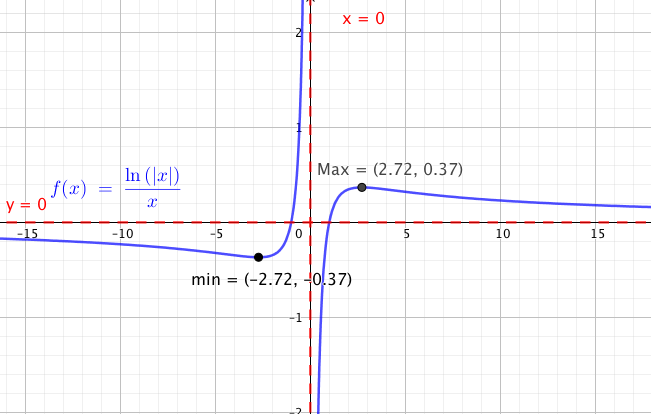
\includegraphics[width=0.7\textwidth]{imagenes/imagenes05/T05IM37.png}
	\end{figure}
	
	Nótese que hemos hecho un cambio en la escala para mejorar la representación.

\end{proofw}


\begin{ejre} Representa la función $y=\dfrac {2x+1}{e^-x}$
	
\end{ejre}

\begin{proofw}\renewcommand{\qedsymbol}{$\diamond$}	


Es evidente que podemos reescribir la función como $y=\dfrac {2x+1}{e^-x}= (2x+1)\cdot e^x$
Dominio: $D(f)=\mathbb R$

Cortes: $x=0 \to y=1\; ; \quad y=0 \to 2x+1=0 \to x=-1/2$ Hay dos cortes con los ejes: $\textbf{(0,1)}$ y $\textbf{(-1/2,0)}$

Asíntotas: estudiemos el comportamiento de $f(x)$ en $\pm \infty$, ya que la exponencial tiene comportamiento distinto-

$\underset {x\to + \infty}{lim}{(2x+1)\cdot e^x}=\infty $

$\underset {x\to - \infty}{lim}{(2x+1)\cdot ex}= [x=-t]\underset {t\to + \infty}{lim}{(2t+1)\cdot e^{-t}}=\underset {t\to + \infty}{lim}{\dfrac {2t+1}{e^t} }= [\infty / \infty: \; L'H] = \underset {t\to + \infty}{lim}{\dfrac {2}{e^t} } = 2/\infty = 0$

!`$\; x\to +\infty \leftrightarrow y \to +\infty \; ; \quad x\to -\infty \leftrightarrow y \to 0 \; $ !

Crecimiento: $y'=2 e^x + (2x+1)e^x=(2x+3)e^x \to PC(y') \leftrightarrow y'=0 \to x=-3/2$


	
Fácilmente comprobamos que $x<-3/2 \to y'<0 \to y\; \searrow\; ; \quad x>-3/2 \to y'>0 \to y\; \nearrow$. Tenemos, pues, un mínimo en $\; \;$ !` $m(-3/2,-2e^{-3/2})$ !

Curvatura e inflexiones: $y''=2e^x+(2x+3)e^x=(2x+5)e^x \to PC(y'') \leftrightarrow y''=0 \to x=-5/2  $ Tenemos una inflexión en !` $I(-5/2, -6e^{-5/2}$ !

	\begin{figure}[H]
		\centering
		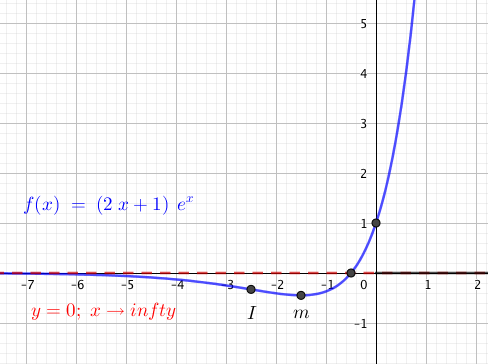
\includegraphics[width=0.75\textwidth]{imagenes/imagenes05/T05IM38.png}
	\end{figure}

	
\end{proofw}

\begin{ejre} Representa $y=2 \sin x + \cos 2x$
	
\end{ejre}

\begin{proofw}\renewcommand{\qedsymbol}{$\diamond$}	

Dominio: $D(f)=\mathbb R$

Periodicidad: como $sin (x)$ es periódica cada $x=2\pi \to T_1=2\pi$; $\cos(2x)$ es periódica cada $2x=2\pi \to T_2=\pi$. El periodo de la función será, si una se repite cada  $T_1=2\pi$ y otra cada $T_2=\pi$, la función se repetirá cada $T=mcm\{T_1, T_2\} \to T=2\pi$. Nos limitaremos a estudiar cortes, máximos y mínimos en $[0,2\pi]$, luego basta con repetor indefinidamente la función.

Cortes: $x=0 \to y=1$; $\quad \textbf{(0,1)}$

$y=0=2 \sin x + \cos 2x \to 2\sin x + (\cos^2 x-\sin^2 x)=0 \to  2\sin x + (1-\sin^2 x x-\sin^2 x)=0 \to -2\sin^2 x +2\sin x +1 =0 \to \sin x = \dfrac {1 \pm \sqrt{3}}{2} $

$x=\arcsin \left(\dfrac {1 + \sqrt{3} } {2} \right) \to \nexists \; x$

$x=\arcsin \left(\dfrac {1 - \sqrt{3} } {2} \right) \to  
\begin{cases}
	x \approx -21.47^o = -21.47  \approx -0.37  rad (+2\pi) \approx 5.91\; rad \\
	x \approx 180^o +21.47^o = \approx \pi+0.37 \approx 3.51 rad 
\end{cases}$


 Tendremos infinitos puntos de corte con OX en  !` $(3.51 \pm 2k\pi,0)\;\wedge \;(5.91 \pm 2k\pi,0)\; \forall k \in Z$ !

Monotonía y extremos: $y'=2\cos x -2\sin (2x)= 2[\cos x - 2 \sin x \; \cos x] = 2 \cos x \; (1-2\sin x) \to PC(y') \leftrightarrow y'=0= 2 \cos x \; (1-2\sin x) \to $

$y'=0 \leftrightarrow $

\noindent \footnotesize{$\begin{cases}{2}
\cos x=0 \to x=90^o = \pi/2 rad \; \wedge \; x= 270^o = 3\pi /2 rad \\
1-2\sin x=0;; \sin x=1/2 \to x=30^o =\pi /6 rad \; \wedge \ x=180^o-30^o = 150^o = 5\pi/6 rad	
\end{cases}$}

\normalsize{Se} deja al lector comprobar si se trata de máximos o mínimos, p.e., aplicando el criterio de la segunda derivada.

!`Hay $\infty \; M \; \wedge \; m: \quad M(\frac \pi 6 + 2k\pi, 1.5); \; M(\frac {5\pi}{6} +2k\pi,1.5); \; m(\frac \pi 2 + 2k\pi, 1); \; m(\frac {3\pi}{2}+2k\pi, -3$ 

Dejamos como ejercicio al lector el estudio de la curvatura e Inflexiones.

	\begin{figure}[H]
		\centering
		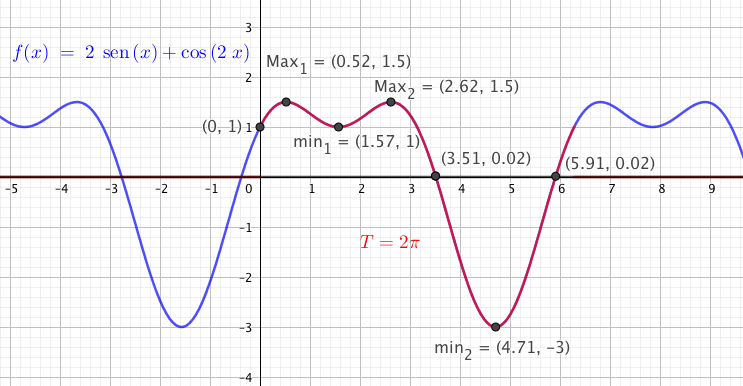
\includegraphics[width=.8\textwidth]{imagenes/imagenes05/T05IM39.png}
	\end{figure}
	
\end{proofw}

\begin{ejre} Representa $y=\dfrac {\sqrt{x^4+1}}{|x|}$
	
\end{ejre}

\begin{proofw}\renewcommand{\qedsymbol}{$\diamond$}	

Obviamente $y=\dfrac {\sqrt{x^4+1}}{|x|}=\begin{cases}
			-\dfrac {\sqrt{x^4+1}}{x} & \mbox{ si } x<0 \\
			\dfrac {\sqrt{x^4+1}}{x} & \mbox{ si } x>0
			\end{cases}\; ; \quad \nexists f(0)$
			
Dominio: $D(f)=\mathbb R \sim \{0\}$

Cortes: $x=0 \to \nexists y\; ; \quad y=0 \to x^4+1\neq 0: \; \nexists x$. No hay puntos de corte.

Asíntotas: Cuidado, las raíces pueden tener comportamiento distinto en $\pm \infty$. No es nuestro caso, pero hemos de estudiar lo que ocurre en $\pm \infty$ porque nuestra función es a trozos.$\underset {x\to 0^{\pm}}{lim}\;{ \dfrac {\sqrt{x^4+1}}{|x|} }= +\infty$, por lo que $\textbf{x=0: \; AV}$.

Al ser el numerador de grado ($4^{\frac 1 2}=2$) mayor al numerador $1$, $\; \underset{x\to \pm \infty}{lim}\; {\dfrac {\sqrt{x^4+1}}{|x|}}=\infty $ y !` $\nexists  \; AH $ !

Vamos a buscar las AO por pasos, cuando $x\to +\infty$ y cuando   $x\to -\infty$:


$\circ \quad x\to +\infty \qquad m=\underset{x\to +\infty}{lim }\;{ \dfrac { \dfrac {\sqrt{x^4+1}} {x} } {x}}= \underset{x\to +\infty}{lim }\;{ \dfrac {\sqrt{x^4+1}}{x^2} }=1$

$n=\underset {x\to +\infty}{lim }\;{ \dfrac {\sqrt{x^4+1}}{x} - x }  = \underset {x\to +\infty}{lim }{ \left(  \dfrac {\sqrt{x^4+1}-x^2}{x} \right)}=[\infty - \infty;:\; ind]=$

$=\underset {x\to +\infty}{lim }{ \left(  \dfrac {\sqrt{x^4+1}-x^2}{x} \right)  \cdot \left(  \dfrac {\sqrt{x^4+1} +1 }{\sqrt{x^4+1} +1}   \right) }= \underset {x\to +\infty}{lim };{ \dfrac {\cancel{x^2}+1+\cancel{x}^2}{x}}=0$. Luego $\textbf{y=x:\; AO}$ por la derecha.

$\circ \quad x\to \infty \qquad$ Se deja al lector, que tras el cambio $[x=-t]$, compruebe que $\textbf{y=-x:\; AO}$ por la izquierda.

Monotonía y extremos. Es fácil comprobar que:

$y'=\begin{cases}
			-\dfrac{x^4-1}{x^2 \sqrt{x^4+1}} & \mbox{ si } x<0 \\
		\dfrac{x^4-1}{x^2 \sqrt{x^4+1}} & \mbox{ si } x>0
			\end{cases}\; ; \quad \nexists f'(0)$

$PC(y') \to \begin{cases}
 \nexists \; y' \leftrightarrow x=0 \\
 y'=0 \leftarrow x^4-1=0 \to x=\pm 1	
 \end{cases}$	
 
 %Estudiemos los signos de $y'$

 
 	\begin{table}[H]
 	\centering
	\begin{tabular}{|c|c|c|c|c|}
	\hline
 	Crecto& $]-\infty,-1[$ & $]-1,0[$ & $]0,1[$ & $]1,+\infty[$ \\ \hline
	$y'$&$-$  & $+$  & $+$  & $-$  \\ \hline
	$y$& $\searrow$ & $\nearrow$ & $\searrow$ & $\nearrow$ \\ \hline
	\end{tabular}
\end{table}



Se observa un $m_1=(-1,\sqrt 2)$ y otro en  $m_2=(1(,\sqrt 2)$

	\begin{figure}[H]
		\centering
		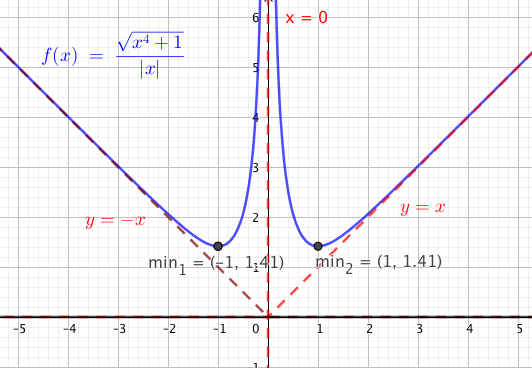
\includegraphics[width=0.7\textwidth]{imagenes/imagenes05/T05IM40.png}
	\end{figure}	
	


\end{proofw} 



\subsection{Ejercicios propuestos de representación de funciones}

\begin{enumerate}
	
	\item  Representa las siguientes funciones:
	
	\begin{enumerate}[a) ]
	\begin{multicols}{2}
	\item $y=x^3+3x*2-x-3$
	\item $y=x^4-3x^2+2$
	\item $y=x^4-4x+3$
	\item $y=\dfrac {3}{x^2-3x}$
	\item $y=\dfrac {x}{1+x^2}$
	\item $y=\dfrac {5-x}{x^2-16}$
	\item $y=\dfrac {(x+3)(x-5)^2}{x^2(x-1)(x-2)^3}$
	\item $y=\dfrac {x^2(x+3)(x-4)}{(x-1)^2(x-3)^2}$
	\item $y=x+\dfrac 1 {x^2}$
	\item $y=\sqrt{1-x^2}$
	\item $y=\sqrt{x^2-1}$
	\item $y=\dfrac {x^2-5x}{x-2}$	
	\end{multicols}
	\end{enumerate}
	

	
	\rightline{\textcolor{gris}{Solución: Ver imagen: Ejercicios propuestos de representación de funciones 1}}
	
	\begin{figure}[]
		\centering
		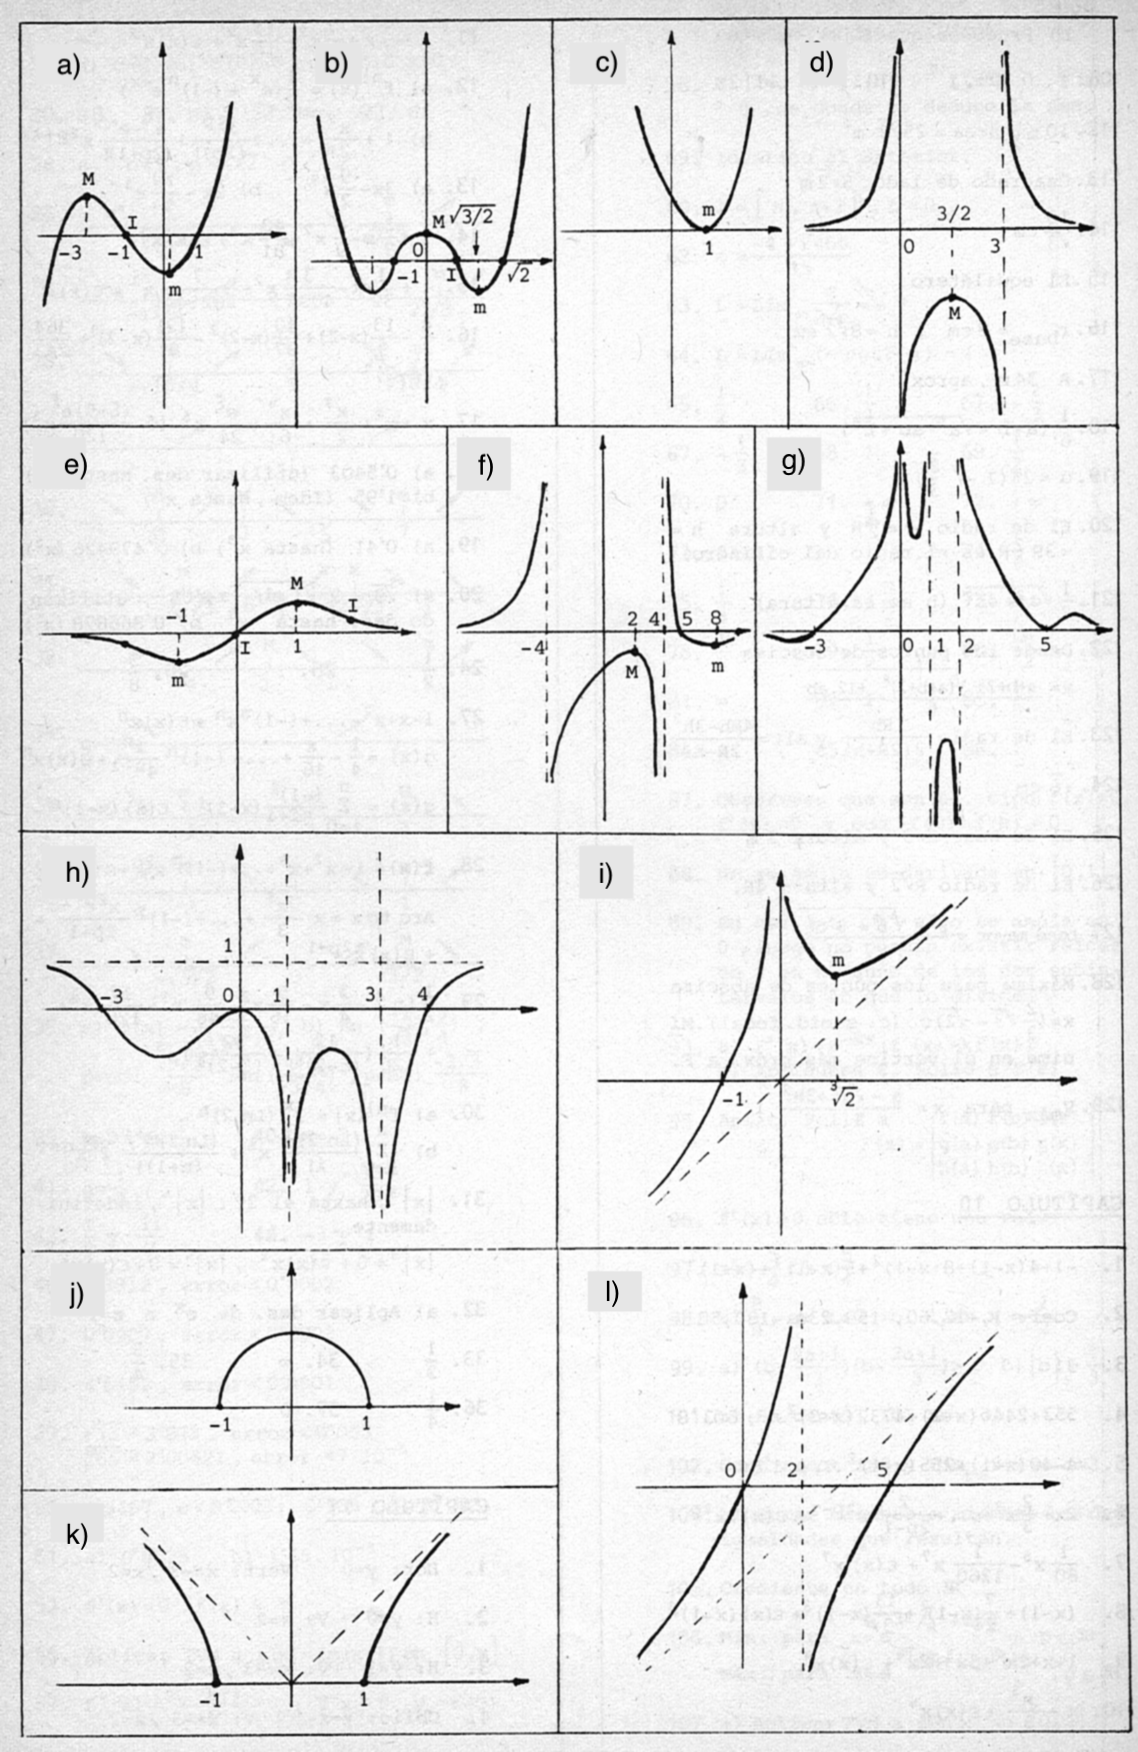
\includegraphics[width=1
		\textwidth]{imagenes/imagenes05/T05IM41.png}
		\caption{Ejercicios propuestos de representación de funciones 1}
	\end{figure}
	
	
	
	\item  Representa las siguientes funciones:
	
	\begin{enumerate}[a) ]
	\begin{multicols}{2}
	\item $y=\dfrac {x^2-2x}{x-5}$
	\item $y=x\; e^x$
	\item $y=x\; e^{-x}$
	\item $y=\dfrac{e^x}{x}$
	\item $y=e^{1/x}$
	\item $y=\dfrac {\mathrm{ln}x}{x}$
	\item $y=\dfrac {x^2}{\sqrt{x^2-1}}$
	\item $y=\dfrac {x}{\sqrt[3]{x^2-1}}$
	\item $y=(\cos x-1)^2$
	\item $y=\mathrm{ln}(x^3-3x+2)$
	\item $y=\dfrac {\cos 3x}{1+\cos 2x}\; \mbox{ en } [0,2\pi]$ (Ayuda: dejar todo en función de $\cos x$)
	
	\end{multicols}
	\end{enumerate}
	
	\rightline{\textcolor{gris}{Solución: Ver imagen: Ejercicios propuestos de representación de funciones 2} }
	
	\begin{figure}[]
		\centering
		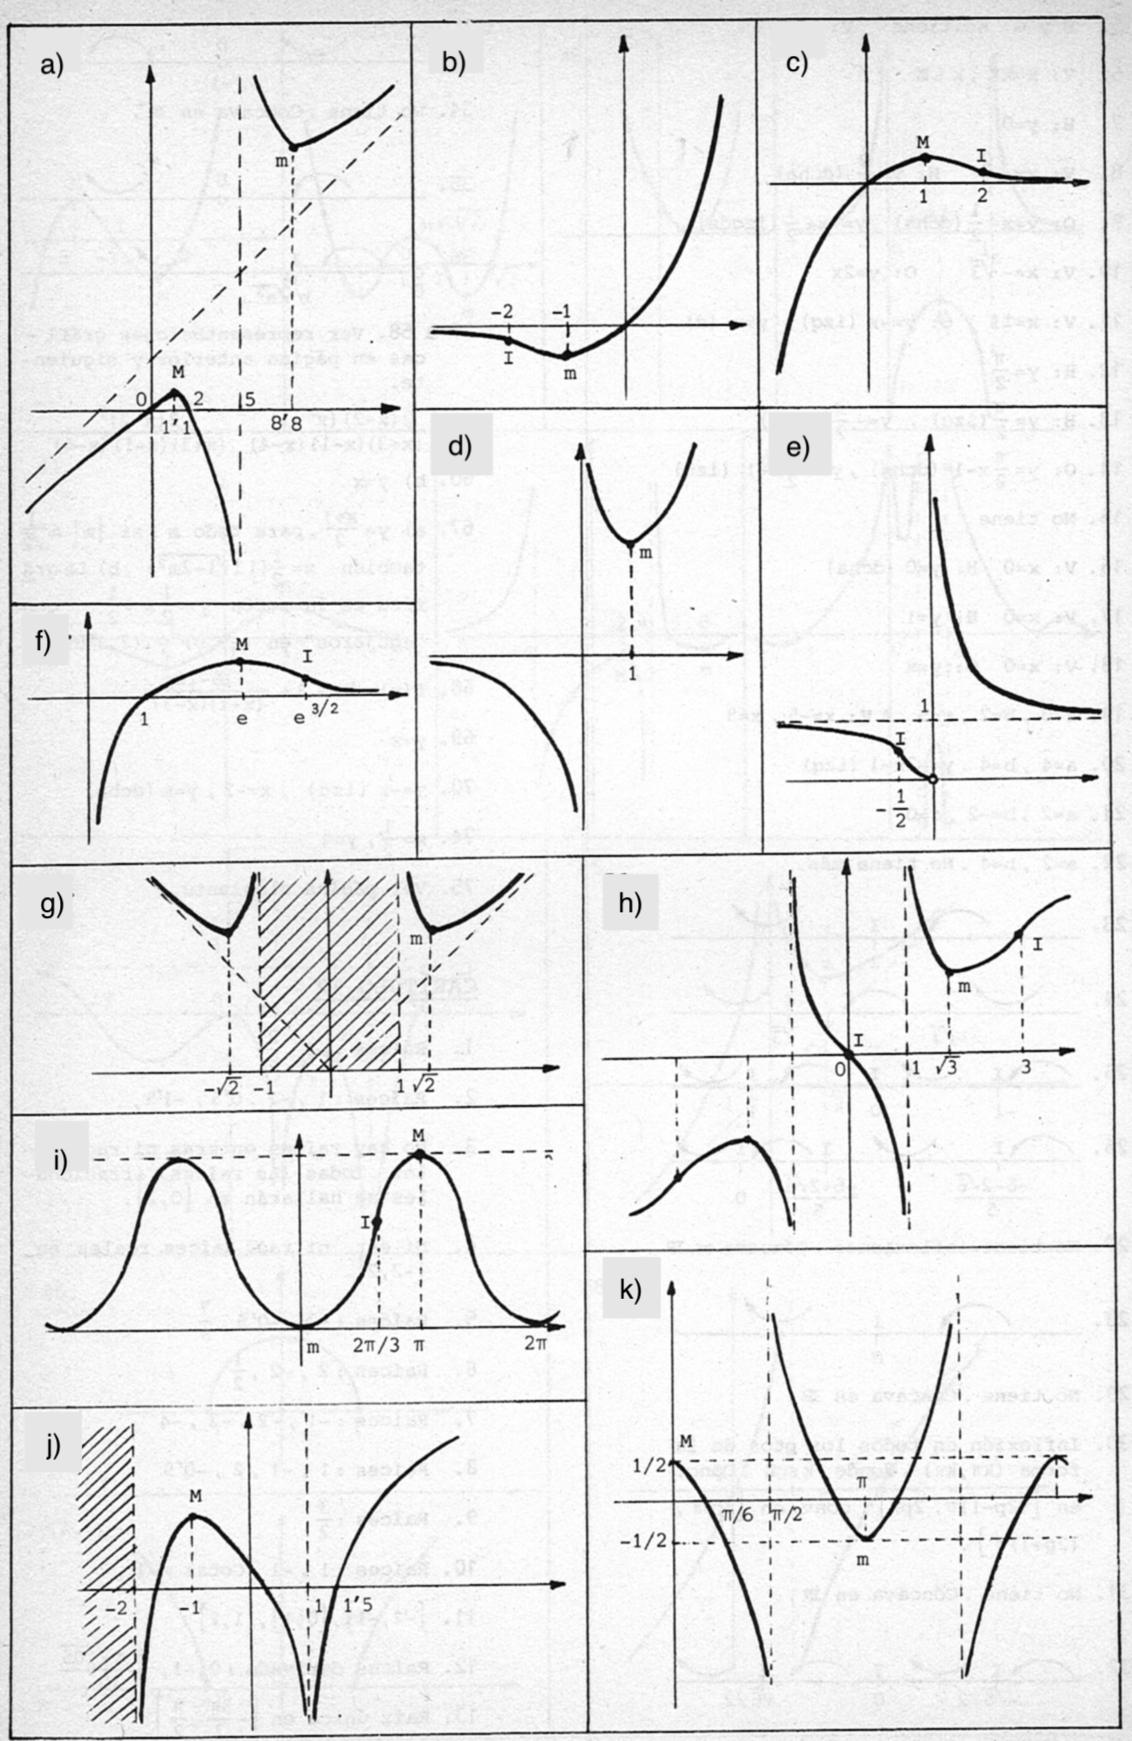
\includegraphics[width=1
		\textwidth]{imagenes/imagenes05/T05IM42.png}
		\caption{Ejercicios propuestos de representación de funciones 2}
	\end{figure}
	
	\item  Representa una función $y=f(x)$ sabiendo que $\underset {x\to +\infty} {lim} \; {f(x)} =0 \; $ ;
	$\underset {x\to -\infty} {lim} \;{\dfrac {f(x)}{x}}=-1 \; $ ; $\underset {x\to -\infty}{lim}\;{ \left( f(x)-(-1)\;x \right) }=-1 \; $ ; $\underset {x\to 2^{\pm}}{lim}\;{f(x)}=+\infty \; $ ; $f(3)=2 \; $ ; $f'(x)=0 \leftrightarrow x=0; \; f(0)=0)$
	
	\rightline{\textcolor{gris}{Solución: Obviamente $y=0$ es AH por la dcha.;}}
	\rightline{\textcolor{gris}{$y=-x-1$ es AO por la izqda.; $x=2$ es AV;}}
	\rightline{\textcolor{gris}{ pasa por $(3,2)$ y hay un extremos (M ó m) en $(0,0)$ }}
	
	\begin{figure}[H]
		\raggedleft
		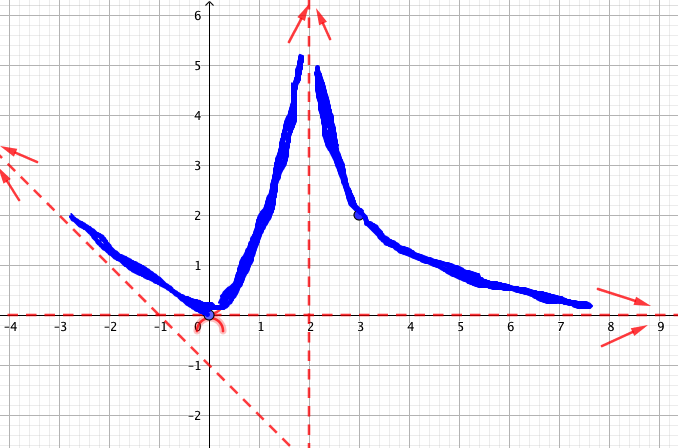
\includegraphics[width=0.4
		\textwidth]{imagenes/imagenes05/T05IM43.png}
		
		\end{figure}
	
	
\end{enumerate}


\section{Ejercicios finales del tema}

Presentamos una colección de problemas  resueltos y propuestos con solución que intenten recoger todo lo aprendido en el tema.

\subsection{Ejercicios resueltos}

	\vspace{5mm}
	\begin{ejre} Estudiar la continuidad y derivabilidad de las siguientes funciones en $x=0$, la gráfica de las cuales aparece en la figura \ref{fig:ctndaddvbdad}
	\end{ejre}
	
	\textcolor{gris}{Verde: no continua en cero; Roja: continua en cero, pero no derivable; azul: continua y derivable en cero.}
	
	$a) \; \textcolor{verd}{f(x)}=\sin \left( \dfrac 1 x \right) \quad 
	b)\; \textcolor{roig}{g(x)}= x\; sin \left( \dfrac 1 x \right) \quad 
	c)\; \textcolor{blau}{h(x)}=x^2\; \sin \left( \dfrac 1 x \right) \quad$
	
	\begin{proofw}\renewcommand{\qedsymbol}{$\diamond$}	
	
	Estudiemos las tres funciones:
	
	$\circ \quad \underset {x\to 0}{lim}\;{f(x)}=\underset {x\to 0}{lim}\;{\sin \left( \dfrac 1 x \right)}=\sin (\infty)=[ \mbox{no existe este límite}]$. Al no poder definir f(0), la función no es continua en cero, luego, obviamente, no derivable.
	
	$f(x)$ no se puede dibujar, de un solo trazo, en un entorno de $0$.
	
	$\circ \quad \underset {x\to 0}{lim}\;{g(x)}=\underset {x\to 0}{lim}\;{x\; sin \left( \dfrac 1 x \right)}= $ [ producto de una función que tiende a cero ($x$) por una función acotada en [-1,1], $\; \sin \left( \dfrac 1 x \right) = 0\cdot k=0; \; \forall\; k\; \in \; [-1,1]$ Basta definir $g(0)=0$ para que $g(x)$ sea ctna. en $x=0$
	
	Veamos ahora que no es derivable en cero, $\nexists \; g'(0)$
	
	$g'(0)=\underset {x \to 0}{lim }\;{\dfrac {g(x)-g(0)}{x-0}}=[\; g(0)=0 \; ]=\underset {x \to 0}{lim}\;{ \dfrac {x\; \; \sin \left( \dfrac 1 x \right)}{x}} = \underset {x\to 0}{lim}\:{\sin \left( \dfrac 1 x \right)}=\sin (\infty)=[ \mbox{no existe este límite}] \to \nexists \; g'(0)$
	
	Aunque $g(x)$ sí se puede dibujar de un solo trazo en un entorno de $0$, es imposible imaginar cómo trazar la recta tangente en $0$. por ello es continua, pero no derivable.
	
	$\circ \quad \underset {x\to 0}{lim}\;{h(x)=}\underset {x \to 0}{lim}\; { x^2\; \sin \left( \dfrac 1 x \right) }$= [ por el mismo motivo que en g(x), cero por un número entre -1 y 1 siempre da cero ] =$0\cdot k=0; \; \forall\; k\; \in \; [-1,1]$. Basta con definir $h(0)=0$ para que $h(x)$ sea ctna. en $0$.
	
	Veamos ahora que sí es derivable en cero, $\exists \; h'(0)$ 
	
	$h'(0)= \underset {x\to 0}{lim }\; { \dfrac {h(x)-h(0)} {x-0}}=[\; h(0)=0 \; ] = \underset {x\to 0}{lim }\; {.\dfrac { x^2\; \sin \left( \dfrac 1 x \right) }{x} = \underset {x\to 0}{lim}\; {x\; \sin \left( \dfrac 1 x \right)}}=0\cdot k=0; \; \forall\; k\; \in \; [-1,1] \to \exists \; h'(0)=0$
	
	La función $h$ se puede dibujar de un solo trazo en un entorno de cero y, claramente, la recta tangente en $x=0$ es horizontal, se puede trazar, luego $h$ es devivable en $0$.
		
		
	Dada la importancia el ejercicio, repetimos la figura	 \ref{fig:ctndaddvbdad}
	
	\begin{figure}[H]
			\centering
			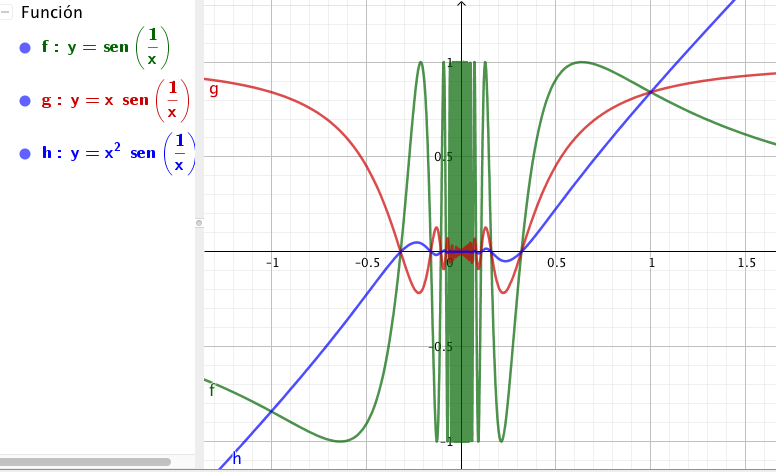
\includegraphics[width=0.7\textwidth]{imagenes/imagenes04/T04IM08.png}
			\caption{Verde: no continua en cero; Roja: continua en cero, pero no derivable; azul: continua y derivable en cero.}
			\label{fig:ctndaddvbdad}
		\end{figure}
		
	\end{proofw} 
		
	\begin{ejre} Calcula los valores de los parámetros $a$, $b$ y $c$ para que la siguiente función cumpla las hipótesis del Th. de Rolle en $[-2,2]$. 
	$y=\begin{cases}
	ax+b\; & x<1 \\
	x^2+cx\; & x\ge 1
	\end{cases}$	
	\end{ejre}
	
	\begin{proofw}\renewcommand{\qedsymbol}{$\diamond$}	
	$y=\begin{cases}
	ax+b\; & x<1 \\
	x^2+cx\; & x\ge 1
	\end{cases} \qquad \to \qquad y'=\begin{cases}
	a\; & x<1 \\
	2x+c\; & x > 1
	\end{cases}$
	
	$y$ e $y'$ son polinóminas: ctnas. y dvbles. en todo $\mathbb R$ excepto quizás en el nexo $x=1$
	
	Continuidad en $x=1$:(método rápido)  $f-(1)=a+b=1+c=f_+(1)$ (*ec-1) 
	
	Derivabilidad en x=1: $f'_-(1)=a=1+c=f'_+(1)$ (*ec-2)
	
	$f(2)=f(-2) \to -2a+b=4+2c$ (*ec-3)
	
	Resolviendo el sistema se obtiene: $a=-1/4 ;\; b=-1 ;\; c=-9/4 ;\; $
	\end{proofw}
	
	\begin{ejre} Desde un punto $O$de la orilla del mar, un nadador debe alcanzar una boya que dista $3km$ de la costa y $3	\sqrt{5} km$ del punto $O$. Si recorriendo la orilla (que suponemos recta y plana) su velocidad media es de $5km/h$ y nadando de $3km/h$, ?`cuánto tiempo deberá caminar hasta lanzarse al mar para alcanzar la boya en el menor tiempo posible?
		
	\end{ejre}
	
	\begin{proofw}\renewcommand{\qedsymbol}{$\diamond$}	
	Hagamos un dibujo del problema:
	
	\begin{multicols}{2}
		\begin{figure}[H]
			\centering
			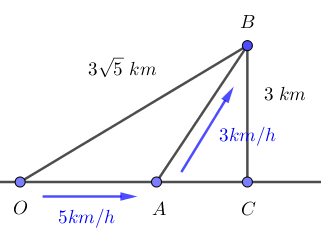
\includegraphics[width=0.3\textwidth]{imagenes/imagenes05/T05IM46.png}
		\end{figure}
	\small{$\overline{OA}$ distancia que recorre por la orilla; $\overline{AB}$ distancia que recorre nadando.}
	
	\small{Llamemos $t_a=x$ al tiempo en $h$ que corre por la orilla: $\overline{OA}=5x\; km$}	
	
	\small{Calculemos por Pitágoras la distancia $\overline{OC}=D \quad  D^2+3^2=(3\sqrt{5})^2 \to D= 6 =\overline{OC}$}

	\end{multicols}



\normalsize{Calculemos} $\overline{AB}$: tenemos un triángulo rectángulo $ACB$ en que $\overline{BC}=3km$ y $\overline{AC}=6-5x$.
	De Pitágoras en $ABC$, obtenemos: $\overline{AB}^2=3^2+(6-5x)^2 \to \overline{AB}=\sqrt{25x^2-60x+45}$ 
	
	El tiempo que invertirá nadando será de ($\; v=s/t \to t=s/v\; $), $\; t_n=\frac 1 5 \sqrt{25x^2-60x+45}$
	
	El tiempo total empleado para ir de $O$ a $B$ será: $t=t_a+t_n=x+\frac 1 5 \sqrt{25x^2-60x+45}$. Obviamente, $x>0$
	
	Para buscar el mínimo de $t$, calculemos $t'$ y busquemos sus $PC(t')$.
	
	$t'=1+ \frac 1 5 \dfrac {50x+-60}{2 \sqrt{25x^2-60x+45}}=
	\dfrac {3\sqrt{5}\sqrt{5x^2-12x+9}+25x-30}{3\sqrt{5}\sqrt{5x^2-12x+9}}$ 
	
	$PV(t'):$ Como el denominador nunca es cero, solo hemos de buscar cuando $t'=0=3\sqrt{5}\sqrt{5x^2-12x+9}+25x-30$; es decir, $3\sqrt{5}\sqrt{5x^2-12x+9}=30-25x\; $ (*). Tenemos una ecuación irracional, con la parte irracional (raíz) aislada en un solo miembro: elevaremos ambos miembros al cuadrado. \emph{!`Cuidado, al provenir de una ecuación irracional, no todas las soluciones pueden ser buenas, habrá que comprobarlas en la ecuación inicial! (*).}
	
	$\left( 3\sqrt{5}\sqrt{5x^2-12x+9} \right)^2 =(30-25x)^2 \to \cdots \to 80x^2-192+99=0 \to x \approx \{1.65; \; 0.75\}$
	
	El lector puede comprobar que $0.75$ es una solución válida, verifica la ecuación (*), pero no así para $1.65$ que no verifica (*).
	
	Luego tenemos un único punto crítico para $t'$, cuando $t=1.65h$. No es difícil comprobar que $0<t<0.75 \to t'<0 \to t\; \searrow; \quad x>0.75 \to t'>0 \to t\; \nearrow  $, lo que confirma que $x=0.75h=45min$ es el tiempo mínimo que ha de andar por la orilla el nadador antes de lanzarse al mar. Dejamos al lector que calcule, si lo desea el tiempo de nado, el tiempo total empleado así como las distancias recorridas a pie y nadando.
	
	\end{proofw}
	
	
	
	\begin{ejre}De todos los cilindros que pueden inscribirse en una esfera de $9m$ de radio, encuentra las dimensiones del que tiene mayor volumen, y el volumen de éste.	
	\end{ejre}
	
	\begin{proofw}\renewcommand{\qedsymbol}{$\diamond$}	
		
		Necesitaremos un dibujo para aclarar el problema.

	
	\begin{multicols}{2}
		
		\begin{figure}[H]
			\centering
			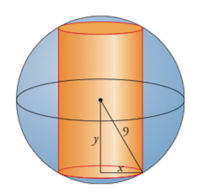
\includegraphics[width=0.4\textwidth]{imagenes/imagenes05/T05IM29.png}
		\end{figure}
		
		Pitágoras: $x^2+y^2=9^2 \to x^2=81-y^2$ (*)
		
		Las dimensiones del cilindro son $r$ y $h=2y$, por lo qe el Volumen es: $V(x,y)=\pi\; r^2\; h = \pi \; r^2 \; 2y = 2\pi \ x^2 \; y$
		
		Teniendo en cuenta la relación (*)= $V(y)=\pi (81-y^2)2y=162\pi \; y - 2\pi \;y^3$
		
		$V'(y)=162\pi - 6\pi \; y^2 \to PC(V'):\; V'=0\to y=\pm 3\sqrt{3}$. Obviamente solo admitimos la solución $y=3\sqrt{3}$
	
	\end{multicols}
	
	Como $y\; \in \; [0,18]$, deberíamos tabular $V$ en $\{0, 3\sqrt{3}, 18\}$, pero dadas las condiciones geométricas del problema no va a ser necesario. Tanto para $y=0$ como para $y=18$ tenemos cilindros de volumen cero (mínimos absolutos), así que $y=3\sqrt{3}$ es la solución del volumen máximo:
	
	Las dimensiones de este cilindro de volumen máximo son $h=2y=6\sqrt{3} \; m$, $r=x=3\sqrt{6} \; m$ y el $V=342\pi \sqrt{3}\;  m^3$
		
	\end{proofw}

	\begin{ejre} Un pueblo está situado en el punto $A (0, 4)$ de un sistema de referencia cartesiano. El tramo de un río situado en el término municipal del pueblo describe la curva $y=x^2/4$ siendo $-6\le x \le 6.$
	 
Obtener razonadamente, la distancia entre un punto $P (x, y)$ 
del río y el pueblo en función de la abcisa $x$ de $P$. El punto o puntos del tramo del río situados a distancia mínima del pueblo. Y  el punto o puntos del tramo del río situados a distancia máxima del pueblo. 
	
	\end{ejre}
	
	\begin{proofw}\renewcommand{\qedsymbol}{$\diamond$}	
	Empecemos con un dibujo:
	
	
	
	\begin{multicols}{2}
	
	$d=d(\overline{AP})= +\sqrt{(x-0)^2+(y-4)^4}=+\sqrt{(x-0)^2+(\dfrac {x^2}{4}-4)^4}=\sqrt{\dfrac {x^4}{16}-x^2+16}; \quad$ con $x\; \in \; [-6,6]$
	
	Ahora solo falta encontrar $d'$ y sus $PC$
	
	$d'=\dfrac {\dfrac {4x^3}{16}-2x}{2\sqrt{\dfrac {x^4}{16}-x^2+16}}$
	
	
		\begin{figure}[H]
			\centering
			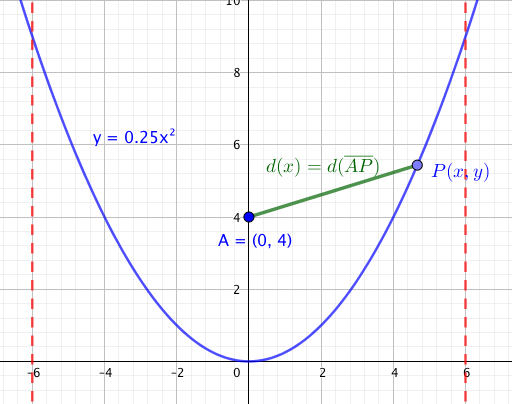
\includegraphics[width=0.4\textwidth]{imagenes/imagenes05/T05IM50.png}
		\end{figure}
	\end{multicols}
	Para averiguar los $PC(d')$, como el denominador representa una distancia y es siempre positivo, bastará con estudiar cuando $d'=0 \to \dfrac {x^3}{4}-2x=0 \to x=\{0, \pm 2\sqrt{2}\}$
	
	Dejamos ya al lector tabular los valores de $d$ en $x=\{0, \pm 2\sqrt{2}\}$ y en $x=\pm 6$, ya que estamos estudiando Máximos y mínimos Absolutos de una función en un intervalo cerrado. La solución es:
	
	La distancia mínima del río al pueblo, que es de $\sqrt{12}m$, se obtiene en los puntos de coordenadas $(\pm2\sqrt{2},2)$ y la distancia máxima de $7.81 m$ aprox., se alcanza en los puntos $(\pm 6,9)$.
	
	
	
	\end{proofw}
	
	\begin{ejre}Las coordenadas iniciales de los móviles $A$ y $B$ son $(0,0)$ y $(250,0)$, respectivamente, siendo $1 km$ la distancia del origen de coordenadas a cada uno de los puntos $(1,0)$ y $(0,1)$. 
	
	El móvil $A$ se desplaza sobre el eje $OY$ desde su posición inicial hasta el punto $(0,375/2)$ con velocidad de $30 km/h$ y, simultáneamente, el móvil $B$ se desplaza sobre el eje $OX$ desde su posición inicial hasta el origen de coordenadas con velocidad de $40 km/h$.Obtener, razonadamente: 
	
	$a)\quad$La distancia  $f(t)$  entre los móviles $A$ y $B$ durante el desplazamiento, en función del tiempo $t$ en horas desde que comenzaron a desplazarse
	
	$c)\quad$El tiempo $T$ que tardan los móviles en desplazarse desde su posición inicial a su posición final, y los intervalos de crecimiento y decrecimiento de la función $f$ a lo largo del trayecto.
	
	$c)\quad$Los valores de $t$ para los que la distancia de los móviles es máxima y mínima durante su desplazamiento y dichas distancias máxima y mínima.	
	\end{ejre}
	
	\begin{proofw}\renewcommand{\qedsymbol}{$\diamond$}	
	Necesitaremos un gráfico que nos aclare el problema:
	
	\begin{multicols}{2}
		\begin{figure}[H]
			\centering
			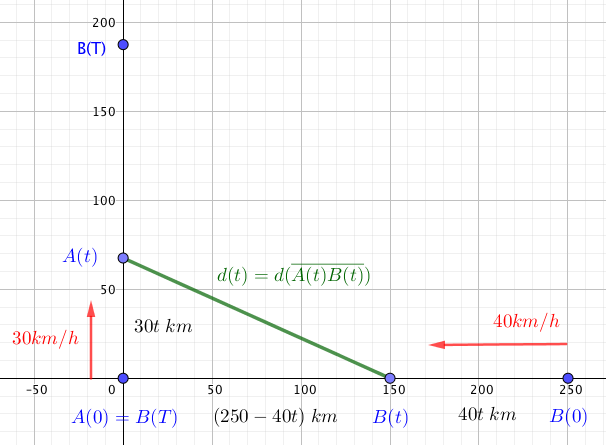
\includegraphics[width=0.5\textwidth]{imagenes/imagenes05/T05IM51.png}
		\end{figure}
		En el primer párrafo del problema nos dice que las unidades de los ejes son $km$. El móvil $A$ deberá recorrer $375/2=187.5 km$ a $30km/h$. Empleará un tiempo en ello $T_A=6.25h$. El móvil $B$ ha de recorrer $250 km$ a $40km/h$, para lo que empleará $T_B=6,25\; h$ (recordad: $v=d/t \to t=d/v$). La respuesta al apartado $b$ es que los dos móviles alcanzan sus objetivos en el mismo tiempo $T=T_A=T_B=6.25h=6h:15min$	
	\end{multicols}
	Al cabo de $t \; (h)$ del comienzo del viaje, el móvil $A$ ha recorrido en el eje $OY$ una distancia de $30t\; km$, ocupará la posición $A(t)=(0,30t)$. El móvil $B$ habrá recorrido $40 t \; km$ hacia el origen de coordenadas, estará pues en la posición $B(t)=(250-40t,0)$. Estos, ($30t$ y $250-40t$) son los catetos de nuestra hipotenusa $d(t)$ que nos da la distancia entre móviles en el instante $t$ y cuya expresión buscamos. Por Pitágoras:
	
	$d(t)=+\sqrt{(30t)^2+(250-40t)^2}=\sqrt{2500t^2-20000t+62500}\; $ , que es la respuesta al apartado $a$
	
	Para responder al apartado $c$, en que nos piden $d$ máx. y min. absolutos en $[0,6.25]\ $ ; buscaremos los puntos críticos de $d'(t)$ en $]0,6.25[$ y tabularemos $d(t)$ el los puntos críticos encontrados y también en los límites del intervalo considerado $t=0$ t $t=6.25$.
	
	$d'(t)=\dfrac {5000t-20000}{2\sqrt{2500t^2-20000t+62500}}$
	
	Como el denominador representa una distancia va a ser siempre positivo y los únicos $PC(d')$ provendrán de $d'=0=5000t-20000 \to t=4\; h$
	
	Sustituyendo de $d(t)$, se obtiene: $\; d(0)=250; \; d(4)=150; \; d(6.25)=187.5 \;  $. Conclusión, los móviles se encuentran a distancia máxima de $250km$ al comienzo del movimiento $t=0\; h$ y se encuentran a la mínima distancia de $150km$ al cabo de $4\; h$ del comienzo del movimiento.
	\end{proofw}
	
	\begin{ejre}
		Determina las dimensiones de una varilla rígida de volumen máximo que puede girar por la esquina recta de un pasillo de $1m$ de anchura.
	\end{ejre}
	

	
	\begin{proofw}\renewcommand{\qedsymbol}{$\diamond$}	
	
	\begin{multicols}{2}
		
	\begin{figure}[H]
		\centering
		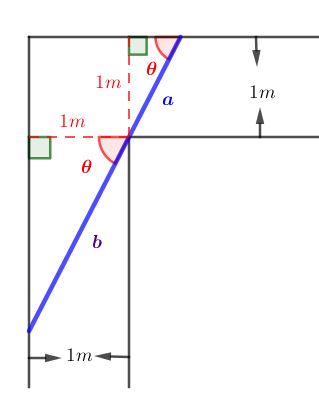
\includegraphics[width=0.35\textwidth]{imagenes/imagenes05/T05IM53.png}
	\end{figure}
		\hspace{5mm}$\sin \theta = \dfrac  {1}  {a} \to a(\theta)= \dfrac {1}{\sin \theta}$ 
		
		$\cos \theta = \dfrac  {1}  {b} \to b(\theta)= \dfrac {1}{\cos \theta}$
		
		Llamamos $L$ a la longitud de la varilla rígida, cuyo máximo queremos determinar. Obviamente:
		
		$L(\theta)=a(\theta)+b(\theta)=\dfrac {1}{\sin \theta} + \dfrac {1}{\cos \theta}$
		
		$L'(\theta)=-\dfrac {\cos \theta}{\sin^2 \theta} - \dfrac {-\cos \theta}{\cos^2 \theta}=\dfrac {\sin^3 \theta - \cos^3 \theta}{\sin^2 \theta \cdot \cos^2 \theta}; \quad \theta\; \in\; ]0,\pi/2[$
	\end{multicols}

	Como en $\theta\; \in\; ]0,\pi/2[ \quad \sin \theta \neq 0 \quad \wedge \quad \cos \theta \neq 0 \quad \to \quad PC(L') \leftrightarrow L'=0$
	
	$L'=0 \to \sin^3 \theta - \cos^3 \theta = 0 \quad \to \quad \sin^3 \theta = \cos^3 \theta \leftrightarrow \sin \theta = \cos \theta \Rightarrow x=\pi/4$	
	
	Como $0<x<\pi/4: \; \sin \theta < \cos \theta \to y'<0 \to y\; \searrow$
	
	Como $\pi/4<x<\pi/2: \; \sin \theta > \cos \theta \to y'>0 \to y\; \nearrow$
	
	Conclusión: en $\theta = \pi/4$ hay un Máximo, de valor $a=\sqrt{2}=b \to L_{max}=2\sqrt{2} \; m$. \textcolor{gris}{(Para un pasillo de anchura $D$, la longitud máxima de una varilla rígida que puede girar es de $L–{max}=2\sqrt{2}D$)}
	
	\end{proofw}

	
	
	
\subsection{Ejercicios propuestos}

\begin{enumerate}

\item Una partícula se mueve a lo largo de la gráfica de la curva $y=f(x)=\dfrac {2x}{1-x^2}$, para x>1. En el punto $P(2,-4/3)$ la deja y se desplaza al lo largo de la recta tangente a dicha curva.

	$\quad a) \quad$ Halla la ecuación de esa recta tangente.
	
	$\quad b) \quad$ Si la partícula se desplaza de derecha a izquierda, halla el punto $Q$ en que la partícula se encuentra a la asíntota vertical más próxima al punto $P$.
	
	$\quad c) \quad$ Si el despazacimiento es de izquierda a derecha, halla el punto $R$ en que la partícula se encuentra en el eje $OX$.
	
\rightline{\textcolor{gris}{Solución: $a) \; RT: \; y = \frac {10}{9}x-\frac {32}{9}; \; b) \; Q(1,-\frac {22}{9});º\; c)\; R(\frac {16}{5},0)$ }}


	
\item Calcula la ecuación de la recta tangente y de la recta normal a la función $f(x)=\dfrac {\mathrm{ln}x}{x}$, en los puntos de corte de $f(x)$ con los ejes coordenados.

\rightline{\textcolor{gris}{Solución: Como $D(f)=\mathrm {R^+_{*}}$, él unico corte es con $OX$ y corta en $x=1$ }}
\rightline{\textcolor{gris}{$RT: \; y=x-1; \quad RN: \; y=-x+1$ }}

\item Hallar el valor de $a$ para el cual la curva $y=2x^3-3x^2+a$ y la recta $y=12x-1$ sean tangentes. ¿Cuál es el punto de tangencia?

\rightline{\textcolor{gris}{Solución: $a=-8; \quad (-1,-13); \quad \vee \quad a=19; \quad (2,23)$}}

\item Hallar $m$ para que la recta tangente a la curva $y=\sqrt{25-x^2}$, en el punto de abcisa $x=4$, sea perpendicular a la recta $y=mx$.

\rightline{\textcolor{gris}{Solución: $m=3/4$}}

\item La recta $y=6x+a$ es tangente a la función $y=\dfrac {bx-1}{bx+1}$, en el punto $x=0$. Calcula $a$ y $b$.

\rightline{\textcolor{gris}{Solución: $a=-1; \; b=3$}} 

\item Si una recta tangente a $x^4-2x^2-x+y=0$, en el pinto $(-1,0)$ es tamnbién tangente a la misma curva en otro punto $P$. determina sus coordenadas.

\rightline{\textcolor{gris}{Solución: $P(1,2)$}}

\item $\divideontimes$ Encuentra las ecuaciones de la RT y RN a la función:
 
$y=\sqrt{5+x^2\sqrt{5+x^2\sqrt{5+x^2\sqrt{\cdots}}}}$, en el punto de abcisa $x=2$.

\rightline{\textcolor{gris}{Solución: Ayuda, recuerda los problemas de ampliación del tema 1 (\ref{curiosidades1})}}
\rightline{\textcolor{gris}{Solución: $RT:\; 10x-3y-5=0; \quad RN\; 3x+10y-56=0$}}

\item Encuentra el valor de los parámetros $a,\; b,\; c\; $ y $\; d\; $, sabiendo que $f(x)=ax^3+bx^2+cx+d$ tiene por recta tangente en el pinto de inflexión $I(1,0); \quad RT:\; 3x+y-3=0$ y que tiene un extremo relativo en $x=0$. ¿El extremo es Máximo o mínimo?

\rightline{\textcolor{gris}{Solución: $a=3;\;b=-9;\;c=6;\;d=0$}}

\item Determina el valor de las constantes $a$, $b$ y $c$ para que $f(x)=x(ax^2+bx+c)$ tenga un punto de inflexión en $x=-2$ y que en dicho punto, la recta tangente tenga por ecuación $10x+y+8=0$ 

\rightline{\textcolor{gris}{Solución: $a=1; \; b=6; \; c=2$}}

\item Hallar los valores de $m$ para que $y=x^4+4x^3+mx^2+3x-2$ sea convexa en todo $\mathrm{R}$.

\rightline{\textcolor{gris}{Solución: $m\ge6$}}

\item Determina un punto de la curva $y=x\; e^{-x^2}$ en que la pendiente de la recta tangente sea máxima.

\rightline{\textcolor{gris}{Solución: $x=0$}}

\item Sea $f(x)=a\sin 3x +b\cos 3x$. Hallar $a$ y $b$ para que se cumpla la igualdad: $f''(x)+4f'(x)+3f(x)=10\cos 3x$.

\rightline{\textcolor{gris}{Solución: $a=2/3; \; b=-1/3$}}

\item 	Se quiere construir un estadio vallado de $1000$ metros 
cuadrados de superficie. El estadio está formado por un 
rectángulo de base x y dos semicírculos exteriores de 
diámetro $x$, de manera que cada lado horizontal del 
rectángulo es diámetro de uno de los semicírculos. El 
precio de un metro de valla para los lados verticales del 
rectángulo es de $1$ euro y el precio de un metro de valla 
para las semicircunferencias es de $2$ euros. Se pide obtener, 
razonadamente: 

La longitud del perímetro del campo en función de x,  el 
coste f(x) de la valla en función de x, así como  el valor de 
x para el que el coste de la valla es mínimo. 

\rightline{\textcolor{gris}{Solución: $P(x)=\dfrac {2000}{x}+\dfrac \pi 2 x^2; \quad \mbox{coste valla: } f(x)=\dfrac {2000}{x}+\dfrac {3\pi} 2 x^2$;}}
 \rightline{\textcolor{gris}{el coste es mínimo para $x \approx 65.15m$}}

\clearpage

\item Resuelve:

\begin {multicols} {2}
	\begin{figure}[H]
		\centering
		\includegraphics[width=0.35\textwidth]{imagenes/imagenes05/T05IM47.png}
	\end{figure}
	
	Para diseñar un escudo se dibuja un triángulo$T$ de vértices $A = (0, 12)$, $B=(x,x^2)$ y $C=(-x,x^2)$, siendo $x^2 <12$.
	
	Obtener, razonadamente, el área del triángulo $T$ en función de la abscisa $x$ del vértice $B$ y las coordenadas de los vértices $B$ y $C$ para que el área del triángulo T sea máxima.
\end {multicols}


\rightline{\textcolor{gris}{Solución: $A(x)=12x-x^3; \quad $}}
\rightline{\textcolor{gris}{Área máxima para $x=2 \to B(2,4); ; C(.2,4)$}}

\item Se desea unir un punto $M$ situado en un lado de una calle, de $6 m$ de anchura, con el punto $N$ situado en el otro lado de la calle, $18 m$ más abajo, mediante dos cables rectos, uno desde $M$ hasta un punto $P$, situado al otro lado de la calle, y otro desde el punto $P$ hasta el punto $N$. 

Se representó la calle en un sistema cartesiano y resultó que $M 
= (0, 6)$ , $P = (x, 0)$ y $N = (18, 0)$ . El cable $MP$ tiene que ser más grueso debido a que cruza la calle sin apoyos 
intermedios, siendo su precio de $10 euros/m$. El precio del 
cable $PN$ es de $5 euros/m$. Obtener, razonadamente: el 
costo total $C$ de los dos cables en función de la abcisa $x$ del punto $P$, cuando $0 \le x \le 18$, y el valor de $x$, con $0\le x\le 18$, para el que el costo total $C$ es mínimo. Calcula también  el valor de dicho costo total mínimo. 

\rightline{\textcolor{gris}{Solución: $C(x)=10\sqrt{x^5+26}+5; \quad $ Coste mínimo para: $\; x=\sqrt{12}m $ }}
\rightline{\textcolor{gris}{Precio mínimo: $\; 141.96 $ euros}}

\item Una empresa decide lanzar una campaña de propaganda de uno de sus productos editando un texto que ocupa $18 cm^2$ en hojas rectangulares impresas a una cara, con márgenes superior e inferior de $2 cm$ y laterales de $1 cm$. Se pide calcular, razonadamente, las dimensiones de la hoja para las que el consumo de papel sea mínimo 

\rightline{\textcolor{gris}{Solución: El papel es mínimo para $5 cm ; \times ; 10cm$}}

\item Un proveedor vende un producto a un comerciante al precio de $300$ euros la unidad. El comerciante incrementa la cantidad de $300$ euros en un $40\%$ para obtener el precio de venta al público. El comerciante sabe que a ese precio 
	venderá $50$ unidades cada mes y que durante el mes de rebajas por cada $3$ euros de reducción en el precio de venta de la unidad conseguirá un incremento de ventas de $5$ unidades. Se pide determinar, razonadamente, el 
número de unidades que debe pedir al proveedor para venderlas en el mes de rebajas y el precio de venta de cada unidad, para maximizar sus beneficios durante ese periodo. 

\rightline{\textcolor{gris}{Solución: Debe pedir $125\; u$ y vender cada unidad a $375$ euros.}}

\item Encuentra las dimensiones de un cilindro circular recto de volumen máximo que puede inscribirse en un cono de radio $R$ y altura $H$.

\rightline{\textcolor{gris}{Solución: El cilindro debe tener $r=2R/3; \; h=H/3; \; V_{ci}=4/9\; V–{co}$}}


\item 

	\begin{multicols}{2}
	De una lámina circular de radio $a$ se quiere cortar un sector circular para formar un cono recto. Si el cono debe tener volumen máximo, ?`cuál ha de ser el ángulo $\theta$ a cortar?
	\begin{figure}[H]
		\centering
		\includegraphics[width=.2\textwidth]{imagenes/imagenes05/T05IM55.png}
	\end{figure}
		
	\end{multicols}
	
\rightline{\textcolor{gris}{Solución: $\theta=\dfrac {2\sqrt{2 \pi}}{\sqrt{3}}$}}

\item Considera una función $f(x)$ que es ctna. y dvble, en todo $\mathrm R$ y tal que $f(0)=0$ y $f(2)=2$. Prueba que existe algún $c\in ]0,2[$ tal que $g'(c)=1$. Enuncia los teoremas que te bases para demostrarlo.

\rightline{\textcolor{gris}{Solución: El teorema del valor medio.}}

\item La función $f(x)$ es ctna. en $[0,5]$ y dvble. en $]0,5[$, además, $f(0)=f(5)$. Calcula, razonadamente, $a$, $b$ y $c$, siendo $f(x)=\begin{cases}
		bx^2 + ax & \mbox{ si } 0 \ge x < 2 \\
		c+\sqrt{x-1} & \mbox{ si } 2 \ge x \ge 5
		\end{cases}$
		
\rightline{\textcolor{gris}{Solución: $a=-3/2; \quad b)=1/2; \quad c=-2$.}}

\item Sea $f(x)=x^3+ax^2+bx+5$. Encuentra $a$ y $b$ para que $f$ tenga en $x=1$ un punto de inflexión de tangente horizontal.

\rightline{\textcolor{gris}{Solución: $a=-3; \quad b=3$}}

\item Determina el valor de $a$ sabiendo que existe y es finito el límite

 
$\underset {x\to 0}{lim}\;{\dfrac {e^x-e^{-x}+ax}{x-\sin x}}$. Calcula dicho límite.

\rightline{\textcolor{gris}{Solución: $a=-2$; límite $=2$}}

\item Calcula los siguientes límites (recuerda que puedes usar infinitésimos equivalentes):
	\begin{multicols}{2}
	\begin{enumerate}
	\item $\underset{x\to 0^+}{lim}\;{\left( \cos x \right)}^{\frac 1 x}$
	\item  $\underset{x\to0}{lim}\;{\dfrac {\sqrt{1+x}-\sqrt{1-x}}{x}}$
	\item  $\underset{x\to 1}{lim}\;{x^{\frac {1}{1-x}}}$
	\item  $\underset{x\to \dfrac {x \cdot \cos x - \sin x}{x^3}}{lim}\;{}$
	\item  $\underset{x\to-\infty}{lim}\;{\left( \dfrac {5-x^2}{3-x^2}\right)}^{\frac {3x^2+1}{2x}}$
	\item  $\underset{x\to 0}{lim}\;{\dfrac {\sin x - \frac 1 2 \sin 2x}{x^3}}$
	\item $\underset{x\to 2}{lim}{\dfrac {\sqrt{13-x^2}-3}{x-2}}$
	\item $\underset{x\to 0}{lim}{\dfrac {x^4 - \frac 1 3 x^3}{x-\tan x}}$
	\item $\underset{x\to 0 }{lim}\; {\dfrac {\mathrm{ln}(1+\sin x)}{\sin x - \tan x}}$
	\item $\underset{x\to 0}{lim}\; {(\tan^2 x)^{\sin x}}$
	\end{enumerate}	
	\end{multicols}

\rightline{\textcolor{gris}{Soluciones: $a)\; ;1\quad b)\; 1/3;\quad c)\; 1/e; \quad d)\; -1/3; \quad e)\; 1$}}
\rightline{\textcolor{gris}{$ f)\; 1/2; \quad g)\; -2/3; \quad h)\; 1\quad i)\; -\infty; \quad j)\; 1 $}}

\item Calcula los siguientes límites (recuerda que puedes usar infinitésimos equivalentes):
	\begin{multicols}{2}
	\begin{enumerate}
	\item  $\underset{x\to +\infty}{lim}\;{\dfrac {e^x}{x^{35}-25}}$
	\item  $\underset{x\to +\infty}{lim}\;{\dfrac {\mathrm{Log}(x^{34}-56)}{2x^2}}$
	\item  $\underset{x\to 0}{lim}\;{\dfrac {1-\cos^2 2x}{3x^2}}$
	\item  $\underset{x\to 0}{lim}\;{\dfrac {e^x-\cos x}{x\; \cos x}}$
	\item  $\underset{x\to 0^+}{lim}\;{x^2 \; \mathrm{ln}x}$
	\item  $\underset{x\to 0}{lim}\;{\dfrac {1-\cos x + \sin^2 2x}{\sin^2 2x}}$
	\item  $\underset{x\to 0}{lim}\;{\dfrac {1+x-e^x}{\sin^2 x}}$	
	\item  $\underset{x\to 0}{lim}\;{\left( \dfrac 1 {x^2}\right)^{\tan x}}$
	\item  $\underset{x\to +\infty}{lim}\;{x\; [\mathrm{ln}(x+1)-\mathrm{ln}(x)]}$
	\item  $\underset{x\to 0}{lim}\;{\dfrac {e^x-x \cos x -1}{\sin x - x +1 -\cos x}}$
	\end{enumerate}	
	\end{multicols}

\rightline{\textcolor{gris}{Soluciones: $a)\; +\infty;\quad b)\; 0;\quad c)\; 0; \quad d)\; 1; \quad e)\; 0$}}
\rightline{\textcolor{gris}{$ f)\; 9/2; \quad g)\; -1/2; \quad h)\; 1 \quad i)\; 1; \quad j)\;  1$}}


\item Calcula el valor de $k$ para que  $\underset{x\to 0}{lim}\;{(e^x+kx)^\frac 1 x}=e^4$ 

\rightline{\textcolor{gris}{Solución: $k=3$}}

\item Calcula las asíntotas de las funciones $f(x)=\dfrac {x+\sqrt{x^2+1}}{x}$ y $g(x)=\dfrac {x^3}{x^2-4x+4}$

\rightline{\textcolor{gris}{Soluciónes: $f(x):\quad x=0:\; AV;	\quad y=1:\;  AH (+\infty); \quad y=0:\; AH (-\infty)$}}
\rightline{\textcolor{gris}{ $g(x):\quad x=2:\; AV; \quad y=x+3:\; AO$}}
 \item Sea $f(x)=\begin{cases}
	-x^2-2x & \mbox{ si } x\ge 0 \\
	x\; \mathrm{ln}x & \mbox{ si } x>0
	\end{cases}$. Estudia la continuidad, derivabilidad, crecimiento y extremos relativos.
	
\rightline{\textcolor{gris}{Solución: $f(x)$ es ctna. y dvble en todo $\mathrm {R} $; $\quad M(-1,1); \quad I(0,0); \quad m(1/e,-1/e)$}}

\item Representa las siguientes funciones:
	\begin{multicols}{2}
	\begin{enumerate}
	\item $f(x)=\dfrac {e^x}{x-2}$
	\item $f(x)=\dfrac {2x+1}{e^{-x}}$
	\item $f(x)=x^2\; e^{2x}$
	\item $\dfrac {x}{\mathrm{ln}x}$
	\item $f(x)=\dfrac {\sin x}{\sin x + \cos x}$
	\item $f(x)=x^2 \; e^{\frac 1 x}$
	\end{enumerate}	
	\end{multicols}

\rightline{\textcolor{gris}{Solución: Imagen adjunta}}
	\begin{figure}[H]
		\centering
		\includegraphics[width=1\textwidth]{imagenes/imagenes05/T05IM54.png}
	\end{figure}
\end{enumerate}




	
	

	
		
